%File: formatting-instructions-latex-2024.tex
%release 2024.0
\documentclass[letterpaper]{article} % DO NOT CHANGE THIS
\usepackage{aaai24}  % DO NOT CHANGE THIS
\usepackage{times}  % DO NOT CHANGE THIS
\usepackage{helvet}  % DO NOT CHANGE THIS
\usepackage{courier}  % DO NOT CHANGE THIS
\usepackage[hyphens]{url}  % DO NOT CHANGE THIS
\usepackage{graphicx} % DO NOT CHANGE THIS
\urlstyle{rm} % DO NOT CHANGE THIS
\def\UrlFont{\rm}  % DO NOT CHANGE THIS
\usepackage{natbib}  % DO NOT CHANGE THIS AND DO NOT ADD ANY OPTIONS TO IT
\usepackage{caption} % DO NOT CHANGE THIS AND DO NOT ADD ANY OPTIONS TO IT
\frenchspacing  % DO NOT CHANGE THIS
\setlength{\pdfpagewidth}{8.5in}  % DO NOT CHANGE THIS
\setlength{\pdfpageheight}{11in}  % DO NOT CHANGE THIS
%
% These are recommended to typeset algorithms but not required. See the subsubsection on algorithms. Remove them if you don't have algorithms in your paper.
\usepackage{algorithm}
% \usepackage{algorithmic}
\usepackage{algpseudocode}
% \usepackage{hyperref}

%
% These are are recommended to typeset listings but not required. See the subsubsection on listing. Remove this block if you don't have listings in your paper.
\usepackage{newfloat}
\usepackage{listings}
\DeclareCaptionStyle{ruled}{labelfont=normalfont,labelsep=colon,strut=off} % DO NOT CHANGE THIS
\lstset{%
	basicstyle={\footnotesize\ttfamily},% footnotesize acceptable for monospace
	numbers=left,numberstyle=\footnotesize,xleftmargin=2em,% show line numbers, remove this entire line if you don't want the numbers.
	aboveskip=0pt,belowskip=0pt,%
	showstringspaces=false,tabsize=2,breaklines=true}
\floatstyle{ruled}
\newfloat{listing}{tb}{lst}{}
\floatname{listing}{Listing}
%
% Keep the \pdfinfo as shown here. There's no need
% for you to add the /Title and /Author tags.
\pdfinfo{
/TemplateVersion (2024.1)
}

% DISALLOWED PACKAGES
% \usepackage{authblk} -- This package is specifically forbidden
% \usepackage{balance} -- This package is specifically forbidden
% \usepackage{color (if used in text)
% \usepackage{CJK} -- This package is specifically forbidden
% \usepackage{float} -- This package is specifically forbidden
% \usepackage{flushend} -- This package is specifically forbidden
% \usepackage{fontenc} -- This package is specifically forbidden
% \usepackage{fullpage} -- This package is specifically forbidden
% \usepackage{geometry} -- This package is specifically forbidden
% \usepackage{grffile} -- This package is specifically forbidden
% \usepackage{hyperref} -- This package is specifically forbidden
% \usepackage{navigator} -- This package is specifically forbidden
% (or any other package that embeds links such as navigator or hyperref)
% \indentfirst} -- This package is specifically forbidden
% \layout} -- This package is specifically forbidden
% \multicol} -- This package is specifically forbidden
% \nameref} -- This package is specifically forbidden
% \usepackage{savetrees} -- This package is specifically forbidden
% \usepackage{setspace} -- This package is specifically forbidden
% \usepackage{stfloats} -- This package is specifically forbidden
% \usepackage{tabu} -- This package is specifically forbidden
% \usepackage{titlesec} -- This package is specifically forbidden
% \usepackage{tocbibind} -- This package is specifically forbidden
% \usepackage{ulem} -- This package is specifically forbidden
% \usepackage{wrapfig} -- This package is specifically forbidden
% DISALLOWED COMMANDS
% \nocopyright -- Your paper will not be published if you use this command
% \addtolength -- This command may not be used
% \balance -- This command may not be used
% \baselinestretch -- Your paper will not be published if you use this command
% \clearpage -- No page breaks of any kind may be used for the final version of your paper
% \columnsep -- This command may not be used
% \newpage -- No page breaks of any kind may be used for the final version of your paper
% \pagebreak -- No page breaks of any kind may be used for the final version of your paperr
% \pagestyle -- This command may not be used
% \tiny -- This is not an acceptable font size.
% \vspace{- -- No negative value may be used in proximity of a caption, figure, table, section, subsection, subsubsection, or reference
% \vskip{- -- No negative value may be used to alter spacing above or below a caption, figure, table, section, subsection, subsubsection, or reference

\setcounter{secnumdepth}{0} %May be changed to 1 or 2 if section numbers are desired.

% The file aaai24.sty is the style file for AAAI Press
% proceedings, working notes, and technical reports.
%

% Title

% Your title must be in mixed case, not sentence case.
% That means all verbs (including short verbs like be, is, using,and go),
% nouns, adverbs, adjectives should be capitalized, including both words in hyphenated terms, while
% articles, conjunctions, and prepositions are lower case unless they
% directly follow a colon or long dash
\title{
% Tentative: 
% Low dimensional representation
% Physics-informed Learning, data and model, integration of the two methods and their advantages

% Physics-informed Learning for Stochastic Optimal and Safety-critical Control

% Efficient Stochastic Optimal and Safety-Critical Control with Dimension Reduction and Physics-Informed Learning

Physics-informed Representation and Learning: Control and Risk Quantification
}
\author{
    %Authors
    % All authors must be in the same font size and format.
    Zhuoyuan Wang\textsuperscript{\rm 1},
    % \thanks{With help from the AAAI Publications Committee.} 
    Reece Keller\textsuperscript{\rm 1},
    Xiyu Deng\textsuperscript{\rm 1}, Kenta Hoshino\textsuperscript{\rm 2}, Takashi Tanaka\textsuperscript{\rm 3}, Yorie Nakahira\textsuperscript{\rm 1}
    % George Ferguson,
    % Hans Guesgen,
    % Francisco Cruz\equalcontrib,
    % Marc Pujol-Gonzalez\equalcontrib
}
\affiliations{
    %Afiliations
    \textsuperscript{\rm 1}Carnegie Mellon University, 
    \textsuperscript{\rm 2}Kyoto University,
    \textsuperscript{\rm 3}University of Texas at Austin
    \\
    % If you have multiple authors and multiple affiliations
    % use superscripts in text and roman font to identify them.
    % For example,

    % Sunil Issar\textsuperscript{\rm 2},
    % J. Scott Penberthy\textsuperscript{\rm 3},
    % George Ferguson\textsuperscript{\rm 4},
    % Hans Guesgen\textsuperscript{\rm 5}
    % Note that the comma should be placed after the superscript

    % 1900 Embarcadero Road, Suite 101\\
    % Palo Alto, California 94303-3310 USA\\
    % email address must be in roman text type, not monospace or sans serif
    \{zhuoyuaw, rdkeller, xiyud\}@andrew.cmu.edu, hoshino@i.kyoto-u.ac.jp, ttanaka@utexas.edu, yorie@cmu.edu
%
% See more examples next
}

%Example, Single Author, ->> remove \iffalse,\fi and place them surrounding AAAI title to use it
\iffalse
\title{My Publication Title --- Single Author}
\author {
    Author Name
}
\affiliations{
    Affiliation\\
    Affiliation Line 2\\
    name@example.com
}
\fi

\iffalse
%Example, Multiple Authors, ->> remove \iffalse,\fi and place them surrounding AAAI title to use it
\title{My Publication Title --- Multiple Authors}
\author {
    % Authors
    First Author Name\textsuperscript{\rm 1},
    Second Author Name\textsuperscript{\rm 2},
    Third Author Name\textsuperscript{\rm 1}
}
\affiliations {
    % Affiliations
    \textsuperscript{\rm 1}Affiliation 1\\
    \textsuperscript{\rm 2}Affiliation 2\\
    firstAuthor@affiliation1.com, secondAuthor@affilation2.com, thirdAuthor@affiliation1.com
}
\fi


% REMOVE THIS: bibentry
% This is only needed to show inline citations in the guidelines document. You should not need it and can safely delete it.
% \usepackage{bibentry}
% END REMOVE bibentry


\usepackage{xcolor}
\usepackage{amsmath}
\usepackage{amsthm}
\usepackage{amsfonts}
\usepackage{graphicx}
\usepackage{caption}
\usepackage{subcaption}
\usepackage{bm}

\newcommand{\todo}[1]{\textcolor{blue}{[TODO: #1]}}
\newcommand{\jacob}[1]{\textcolor{blue}{[Jacob: #1]}}
\newcommand{\overview}[1]{{\leavevmode\color{red}#1}}
\newcommand{\resolved}[1]{}

\newcommand{\ie}{\textit{i.e., }}
\newcommand{\eg}{\textit{e.g., }}
\newcommand{\pr}{\mathbb{P}}
\newcommand{\safe}{\mathcal{C}}

\DeclareMathOperator*{\argmax}{arg\,max}
\DeclareMathOperator*{\argmin}{arg\,min}

% \theoremstyle{definition}
% \newtheorem{definition}{Definition}
% \newtheorem{theorem}{Theorem}

\newtheorem{theorem}{Theorem}
\newtheorem{lemma}[theorem]{Lemma}
\newtheorem{proposition}[theorem]{Proposition}
\newtheorem{corollary}[theorem]{Corollary}
\newtheorem{definition}[theorem]{Definition}
\newtheorem{remark}[theorem]{Remark}
\newtheorem{assumption}[theorem]{Assumption}

% tikz for plot
\usepackage{tikz}
\usepackage{xcolor}
\usepackage{verbatim}
\usepackage{multirow}
\usepackage{color}
\usepackage{colortbl}
\usepackage{pgfplots}
\DeclareUnicodeCharacter{2212}{}
\usepgfplotslibrary{groupplots,dateplot}
\usetikzlibrary{patterns,shapes.arrows}
\pgfplotsset{compat=newest}
\usetikzlibrary{shapes.arrows}
\usetikzlibrary{arrows.meta} 
\usetikzlibrary{positioning, fit, shapes.geometric}
\usetikzlibrary{backgrounds}
\definecolor{newblue}{RGB}{189,215,239} 
\definecolor{newgray}{RGB}{214,214,214} 
\definecolor{neworange}{RGB}{241,205,177} 
\definecolor{newyellow}{RGB}{251,231,163} 
\definecolor{newgreen}{RGB}{202,223,184} 
\definecolor{cmured}{RGB}{196,18,48} % Red
\definecolor{cmuskibored}{RGB}{147,17,32} % Skibo Red
\definecolor{cmuyellow}{RGB}{253,181,21} % Yellow
\definecolor{cmublue}{RGB}{4,54,115} % Blue
\definecolor{cmutan}{RGB}{188,180,158} % Tan
\definecolor{cmuteal}{RGB}{31,76,76} % Teal
\definecolor{cmugreen}{RGB}{113,159,148} % Green
\definecolor{cmuskyblue}{RGB}{0,123,192} % Sky Blue
\definecolor{cmuirongray}{RGB}{109,110,113} % Iron Grey
\definecolor{cmugray}{RGB}{244,244,244} % Iron Grey
% \usepackage{filecontents}
\usepackage{pgfplots}
\usepackage{makecell}
\usepgfplotslibrary{fillbetween}
\begin{filecontents*}{pinn_epoch.dat}
    x y err
    10000  7.104  0.025882
    20000  5.322  0.02009
    30000  5.475  0.02065
    40000  5.940  0.022517
    50000  4.733  0.018146
    60000  4.809 0.018371
\end{filecontents*}
\begin{filecontents*}{pinn_pde.dat}
    x y err
    100 5.498 0.020817
    200 5.391 0.02022523
    300 5.749 0.02171
    400 5.927 0.022209
    500 5.478 0.02058
    600 5.283 0.019888
    1200 5.153 0.01962
    2400 4.992 0.01894
\end{filecontents*}
\begin{document}

\maketitle

\begin{abstract}
Optimal and safety-critical control are fundamental problems for stochastic systems, and are widely considered in real-world scenarios such as robotic manipulation and autonomous driving. In this paper, we consider the problem of efficiently finding optimal and safe control for high-dimensional systems. Specifically, we propose to use dimensionality reduction techniques from a comparison theorem for stochastic differential equations together with a generalizable physics-informed neural network to estimate the optimal value function and the safety probability of the system. The proposed framework results in substantial sample efficiency improvement compared to existing methods. We further develop an autoencoder-like neural network to automatically identify the low-dimensional features in the system to enhance the ease of design for system integration. We also provide theoretical analysis and experiments to validate the efficacy of the proposed method. 
% Source code is available at {https://github.com/jacobwang925/path-integral-PINN}.

\end{abstract}

\section{Introduction}

Optimal control and safety-critical control are the two central concerns for autonomous systems.
% Real world applications includes industrial robots, autonomous driving cars, etc.
These concerns are particularly pronounced in real-world applications, including manufacturing robots and autonomous cars.
The operational environment often introduces stochastic noise, which compounds the difficulties of achieving optimal performance and ensuring safety. Traditional deterministic methods prove inadequate for stochastic dynamics~\cite{katsoulakis2020data}.
Furthermore, many real-world systems are characterized by high-dimensional state spaces (\eg multi-agent systems), leading to substantial computational burdens when devising optimal and safe control strategies. 

% In such systems there are often time random noise that impose further challenges for optimal and safe control, as standard deterministic methods do not work anymore. Further more, when the dimension of the system is high, it is hard to find such controls efficiently as the calculation for value function and risk probability are high non-trivial.

Previous work on stochastic optimal control deals with diverse uncertainty and randomness, but these methods are not efficient for high-dimensional systems because forward rollouts and backward dynamic programming requires computation that scales exponentially with the dimension of the state.~\cite{gorodetsky2018high, frankowska2020necessary}\resolved{to elaborate}.
Previous studies on stochastic safe control aim to control the level of risk in the system for a certain period of time, and ensure the probability of safety does not decay over time~\cite{samuelson2018safety,gomez2016real}.
These methods rely on accurate estimation of the probability of risk in the system, and standard methods for such risk estimation are computationally heavy, especially for high-dimensional systems.
For both problems, existing methods require computation that scales linearly with the time horizon of interest. To the best of our knowledge, there is no study that provides generalization of the value function and risk probability in the time horizon, which can be very beneficial for efficient computation in systems with long-term performance requirements.

In order to address these challenges, this study proposes a unified framework to efficiently estimate the value function and safety probability of high-dimensional stochastic systems. The method leverages a comparison theorem~\cite{10.1215/kjm/1250523321} to find low-dimensional representations of the value function and safety probability, and uses such low-dimensional features to construct low-dimensional partial differential equations (PDEs) for the value function and safety probability calculation in order to reduce the dimension of the problem for efficient computation.
% The key insight is that we exploit the possible low-dimensional structure of the high-dimensional value function and safety probability, to reduce the dimension of the problem for efficient computation.
We further propose a physics-informed neural network (PINN) to solve these PDEs for better sample complexity and generalization abilities.
We also propose an autoencoder-like neural network to automatically identify low-dimensional features of the system, and provide error analysis incurred from the process.
Fig.~\ref{fig:overall_diagram} shows the overall diagram of the proposed method. 
The advantages of the proposed method are
\begin{enumerate}
    \item A unified framework for accurate estimation of value functions and safety probabilities of stochastic systems (Fig.~\ref{fig:PINN diagram}). 
    \item Efficient estimation with much lower sample complexity for high-dimensional systems (Fig.~\ref{fig:sample_complexity}).
    \item Generalization to unseen regions in the state space and longer time horizons (Fig.~\ref{fig:value_func_visual} and Fig.~\ref{fig:safe_prob_3d->2d}).
    % and fast inference during test time.
    \item Intuitive plug and use with automatic feature identification (Fig.~\ref{fig:AE diagram}).
\end{enumerate}

% \todo{explain the diagram}
\begin{figure}
    \centering
    % 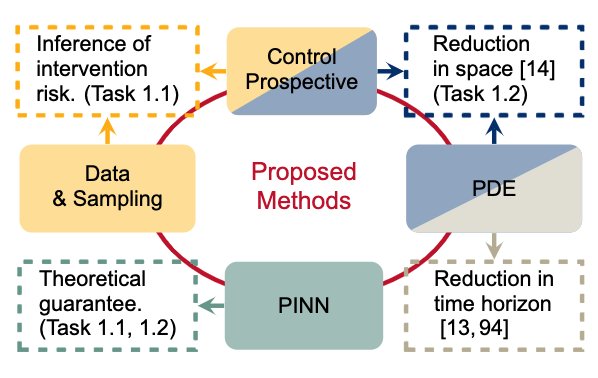
\includegraphics[width=0.4\textwidth]{Figures/overall_diagram_example.png}
    %%%%%%%%%%
% by Xiyu
%%%%%%%%%%%

% color
\definecolor{color5}{HTML}{F2CC8F}
\definecolor{color2}{HTML}{F4F1DE}
\definecolor{color3}{HTML}{3D405B}
\definecolor{color4}{HTML}{81B29A}
\definecolor{color1}{HTML}{E07A5F}
\tikzset{
diagonal fill/.style 2 args={fill=#2, path picture={
\fill[#1, sharp corners] (path picture bounding box.south west) -|
                         (path picture bounding box.north east) -- cycle;}},
reversed diagonal fill/.style 2 args={fill=#2, path picture={
\fill[#1, sharp corners] (path picture bounding box.north west) |- 
                         (path picture bounding box.south east) -- cycle;}}
}

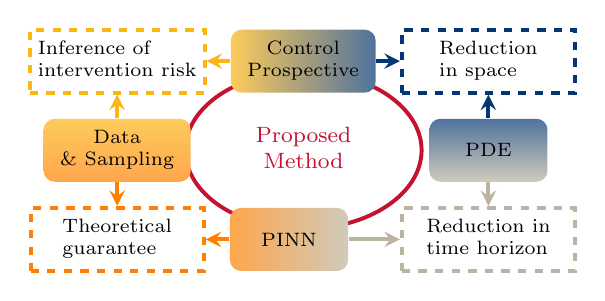
\begin{tikzpicture}[
    node distance = 4cm,
    node/.style={circle, fill=#1, inner sep=2pt, minimum size=0.7cm}, 
    edge/.style={-stealth, #1}
]

% 
\node[rectangle, draw=cmuyellow, dashed, line width=0.5mm, minimum height=0.8cm,minimum width=2.2cm,inner sep=-3pt] (t1){\scriptsize \begin{tabular}{ll}
% Observed data \\ to infer vs \\ the risk of\\ intervention.
Inference of \\ intervention risk
\end{tabular}};
\node[shading = axis, rectangle, left color= cmuyellow!70, right color= cmublue!70, minimum height=0.8cm,minimum width=1.5cm, rounded corners,inner sep=0pt] (control)[right=0.3cm of t1] {\scriptsize \begin{tabular}{cc}
Control \\ Prospective
\end{tabular}};

\node[rectangle, draw=cmublue, dashed, line width=0.5mm, minimum height=0.8cm,minimum width=2.2cm,inner sep=0pt] (t2) [right=0.3cm of control]{\scriptsize \begin{tabular}{ll}
Reduction \\ in space
\end{tabular}};

\node[shading = axis, rectangle, top color= cmuyellow!70, bottom color= orange!70, minimum height=0.8cm,minimum width=1.5cm, rounded corners, inner sep = 0pt] (sr) [below=0.3cm of t1] {\scriptsize \begin{tabular}{cc}
Data \\ \& Sampling\\
\end{tabular}};

\begin{scope}[on background layer]
\node[ellipse, draw = cmured, line width=0.5mm, minimum width = 3cm, minimum height = 2cm, rounded corners] (pm)[right= -0.1 cm of sr]{\footnotesize \textcolor{cmured}{\begin{tabular}{cc}
Proposed \\Method
\end{tabular}}};
\end{scope}

\node[shading = axis, rectangle, top color= cmublue!70, bottom color= cmutan!70, minimum height=0.8cm,minimum width=1.5cm, rounded corners] (pde) [below=0.3cm of t2] {\scriptsize PDE};

\node[rectangle, draw=orange, dashed, line width=0.5mm, minimum height=0.8cm,minimum width=2.2cm,inner sep=0pt] (t3)[below=0.3cm of sr]{\scriptsize \begin{tabular}{ll}
Theoretical \\ guarantee
\end{tabular}};

\node[shading = axis, rectangle, left color= orange!70, right color= cmutan!70,  minimum height=0.8cm,minimum width=1.5cm, rounded corners] (pinn)[right=0.3cm of t3]{\scriptsize PINN};

\node[rectangle, draw=cmutan, dashed, line width=0.5mm, minimum height=0.8cm,minimum width=2.2cm] (pw)[below=0.3cm of pde,inner sep=0pt]{\scriptsize \begin{tabular}{ll}
% Reduction in \\ time horizon \\due to PDE\\ constrains.
Reduction in \\ time horizon 
\end{tabular}};

%Edges
\draw[edge=cmuyellow,line width=0.5mm] (control) -> (t1);
\draw[edge=cmublue,line width=0.5mm] (control) -> (t2);
\draw[edge=cmuyellow,line width=0.5mm] (sr) -> (t1);
\draw[edge=cmublue,line width=0.5mm] (pde) -> (t2);
\draw[edge=orange,line width=0.5mm] (pinn) -> (t3);
\draw[edge=cmutan,line width=0.5mm] (pde) -> (pw);
\draw[edge=cmutan,line width=0.5mm] (pinn) -> (pw);
\draw[edge=orange,line width=0.5mm] (sr) -> (t3);
\end{tikzpicture}


% \begin{tikzpicture}[
%     node distance = 4cm,
%     node/.style={circle, fill=#1, inner sep=2pt, minimum size=0.7cm}, 
%     edge/.style={-stealth, #1}
% ]

% % 
% \node[rectangle, fill=newyellow,  line width=0.5mm, minimum height=0.8cm,minimum width=1.8cm,inner sep=-3pt] (t1){\scriptsize \begin{tabular}{ll}
% % Observed data \\ to infer vs \\ the risk of\\ intervention.
% Inference of \\ cost and risk
% \end{tabular}};

% \node[rectangle,  draw, line width = 0.3mm, minimum height=0.8cm,minimum width=1.8cm, inner sep=0pt] (control)[right=0.5cm of t1] {\scriptsize \begin{tabular}{cc}
% Control \\ Prospective
% \end{tabular}};

% % \node[rectangle,draw=cmuyellow,dash pattern= on 3pt off 5pt,line width = 0.3mm, minimum height=0.8cm,minimum width=1.8cm, inner sep=0pt,postaction={draw,cmublue,dash pattern= on 3pt off 5pt,dash phase=4pt,thick}] (control)[right=0.3cm of t1] {\scriptsize \begin{tabular}{cc}
% % Control \\ Prospective
% % \end{tabular}};


% \node[rectangle, fill=newblue,  line width=0.5mm, minimum height=0.8cm,minimum width=1.8cm,inner sep=0pt] (t2) [right=0.5cm of control]{\scriptsize \begin{tabular}{ll}
% Reduction \\ in space
% \end{tabular}};

% \node[draw, line width = 0.3mm, rectangle, minimum height=0.8cm,minimum width=1.8cm,  inner sep = 0pt] (sr) [below=0.3cm of t1] {\scriptsize \begin{tabular}{cc}
% Data \\ \& Sampling\\
% \end{tabular}};

% % \node[rectangle,draw=orange,dash pattern= on 3pt off 5pt,line width = 0.3mm, minimum height=0.8cm,minimum width=1.8cm, inner sep=0pt,postaction={draw,cmuyellow,dash pattern= on 3pt off 5pt,dash phase=4pt,thick}] (sr)[below=0.3cm of t1] {\scriptsize \begin{tabular}{cc}
% % Data \\ \& Sampling\\
% % \end{tabular}};

% % \begin{scope}[on background layer]
% % \node[rectangle, line width=0.5mm, minimum width = 3cm, minimum height = 2cm, rounded corners] (pm)[right= -0.1 cm of sr]{\scriptsize \begin{tabular}{cc}
% % Proposed \\Method
% % \end{tabular}};
% % \end{scope}

% \node[rectangle, minimum height=0.8cm,minimum width=1.8cm,  inner sep = 0pt] (pm) [below=0.3cm of control] {\footnotesize \begin{tabular}{cc}
% \underline{Proposed Method}
% % Proposed Method
% \end{tabular}};

% \node[rectangle, draw, line width = 0.3mm, minimum height=0.8cm,minimum width=1.8cm] (pde) [below=0.3cm of t2] {\scriptsize PDE};

% % \node[rectangle,draw=cmublue,dash pattern= on 3pt off 5pt,line width = 0.3mm, minimum height=0.8cm,minimum width=1.8cm, inner sep=0pt,postaction={draw,cmutan,dash pattern= on 3pt off 5pt,dash phase=4pt,thick}] (pde)[below=0.3cm of t2] {\scriptsize \begin{tabular}{cc}
% % PDE
% % \end{tabular}};

% \node[rectangle, fill=neworange,  line width=0.5mm, minimum height=0.8cm,minimum width=1.8cm,inner sep=0pt] (t3)[below=0.3cm of sr]{\scriptsize \begin{tabular}{ll}
% Theoretical \\ guarantee
% \end{tabular}};

% \node[rectangle, draw, line width = 0.3mm,  minimum height=0.8cm,minimum width=1.8cm] (pinn)[right=0.5cm of t3]{\scriptsize PINN};

% % \node[rectangle,draw=cmutan,dash pattern= on 3pt off 5pt,line width = 0.3mm, minimum height=0.8cm,minimum width=1.8cm, inner sep=0pt,postaction={draw,orange,dash pattern= on 3pt off 5pt,dash phase=4pt,thick}] (pinn)[right=0.3cm of t3] {\scriptsize \begin{tabular}{cc}
% % PINN
% % \end{tabular}};

% \node[rectangle, fill=newgray,  line width=0.5mm, minimum height=0.8cm,minimum width=1.8cm] (pw)[below=0.3cm of pde,inner sep=0pt]{\scriptsize \begin{tabular}{ll}
% % Reduction in \\ time horizon \\due to PDE\\ constrains.
% Reduction in \\ time horizon 
% \end{tabular}};

% %Edges
% \draw[edge=cmuyellow,line width=0.5mm] (control) -> (t1);
% \draw[edge=cmublue,line width=0.5mm] (control) -> (t2);
% \draw[edge=cmuyellow,line width=0.5mm] (sr) -> (t1);
% \draw[edge=cmublue,line width=0.5mm] (pde) -> (t2);
% \draw[edge=orange,line width=0.5mm] (pinn) -> (t3);
% \draw[edge=cmutan,line width=0.5mm] (pde) -> (pw);
% \draw[edge=cmutan,line width=0.5mm] (pinn) -> (pw);
% \draw[edge=orange,line width=0.5mm] (sr) -> (t3);
% \end{tikzpicture}
    \caption{The overall diagram of the proposed method for stochastic optimal value function and safety probability estimation. \resolved{remove task x.x and replace with content in this paper}
    }
    \label{fig:overall_diagram}
\end{figure}

\vspace{-0.5em}


% The rest of the paper is organized as follow. We introduce the related work in section~\ref{sec:related_work}. We give the formulation of the problem in section~\ref{sec:problem_formulation}. We present our proposed method in section~\ref{sec:proposed_method}. We show the experiment results in section~\ref{sec:experiments}. Finally we conclude the paper in section~\ref{sec:conclusion}.



% \todo{advantages}
% better sample complexity
% better computation time
% better accuracy and generalization

\section{Related Work}
\label{sec:related_work}
% \subsection{Stochastic Optimal Control}
\subsection{Path Integral Optimal Control}
 Path integral control generally refers to numerical methods to solve a stochastic optimal control problem by keeping performing forward Monte Carlo rollouts of open-loop dynamics. The original derivation of the path integral control algorithm~\cite{kappen2005path} relied on the Feynman-Kac lemma, whereas an alternative derivation without the Feynman-Kac lemma became available later~\cite{theodorou2012relative} based on the variational approach. In both derivations, the path integral method is restricted to the class of stochastic optimal control problems whose HJB PDEs are linearizable, but generalizations have been considered in~\cite{satoh2016iterative,williams2017information}. Various implementations such as path integral for policy improvements~\cite{theodorou2010generalized} and receding horizon implementations~\cite{williams2017model} have been widely used. Path integral control has also been applied to constrained systems and systems with non-differentiable dynamics~\cite{satoh2020nonlinear,carius2022constrained}. Path integral control for risk minimization in robot navigation has been considered in~\cite{patil2022chance}, which requires solving PDEs whose dimension scales with the size of the system. Here, we show that the value function and safety probability can be bounded exactly by the solution of two-dimensional PDEs regardless of the system dimension. 
% Stochastic optimal control is widely considered in many engineering applications, such as mechanical systems, chemical plants, finance, and robotics~\cite{} \todo{cite}.
% Optimal control theory provides an elegant mathematical framework for computing an optimal controller using
% the Hamilton-Jacobi-Bellman (HJB) equation. In general the HJB equation is impossible to solve analytically,
% and numerical solutions are intractable due to the problem of dimensionality.
% Previous studies instead consider infinite-time-average cost problems and finite-time problems to linearize the HJB equation for efficient computation, and eigenvalue methods and path integral methods have been developed to solve these problems~\cite{kinjo2013evaluation, theodorou2012relative, horowitz2014linear, kappen2005linear}. These methods allow possible evaluation of the optimal control for low-dimensional systems with short time horizon. However, solving high-dimensional linearized HJB equations explicitly using dynamics programming or implicitly using path integrals are still non-trivial and generalization to longer time horizons remain an open challenge. In this work we fundamentally address the problem of dimensionality by finding low-dimensional representations of the high-dimensional system without sacrificing performance. And we use physics-informed neural networks to generalize the optimal value function estimation from short to long time horizon to further enhance the sample complexity.


% The goal is to find control actions that minimizes the expected cost on the system over a certain period of time. 


% \subsection{Stochastic Safe Control}
\subsection{Risk Quantification for Safe Control}
\resolved{similar topic but alternative objectives, or just cite related safe control papers}
\resolved{add more recent papers on risk quantification}

Risk quantification is the key enabler for many long-term stochastic safe control methods~\cite{wang2021myopically,jing2022probabilistic}.
Existing methods often use rare event simulation through Monte Carlo (MC) and importance sampling to estimate the long-term risk in stochastic systems~\cite{ botev2013markov,hanna2021importance,stadie2018some,madhushani2020hamiltonian}. Subset simulation calculates the risk probability conditioned on intermediate failure events for improved sample efficiency~\cite{huang2016assessing, zhao2022subset, rashki2021sesc}. Probabilistic reachability estimates the risk of controllers in stochastic systems by propagating the estimated risk backwards over time~\cite{hewing2018stochastic,bansal2020hamilton,huh2020safe}. MC techniques typically require the samples to cover states and evaluate the risk over the time horizon.
PDE techniques are also used to understand probabilistic values in stochastic systems~\cite{chern2021safe,feng2014comparative}, but numerical PDE techniques such as finite difference, finite element, and finite volume methods are less scalable than MC methods. 
Probability bounds and martingale inequalities have been used to approximate risk probabilities for certain classes of systems~\cite{clark2019control,yaghoubi2020risk,santoyo2021barrier,cheng2020safe, meng2022sufficient, nishimura2023control}. 
The large deviation is another standard approach that can be adapted to the safe control area, which allows evaluating the probability of the state of a stochastic differential equation that exists from a given region~\cite{bressloff2014path,bertini2015large}. 
Nonetheless, most existing methods suffer from the curse of dimensionality. In this work, we solve the high-dimensional safety probability estimation problem by finding effective low-dimensional representations, and we are able to reduce the sample complexity by orders compared to MC methods.

% Stochastic safe control has been extensively studied as safety under uncertainties and noises is one of the key challenges in real-world autonomous systems. Most of the existing stochastic safe control methods (\eg stochastic reachability~\cite{abate2008probabilistic, prandini2008application, patil2022upper}, Conditional Value-at-Risk~\cite{samuelson2018safety, singletary2022safe}, chance-constrained predictive control~\cite{nakka2020chance, zhu2019chance, pfrommer2022safe}) require accurate estimation of risk probabilities or their gradients to yield desirable performance, and to get accurate estimates itself challenging. Rare event simulation methods aim to find small risk probabilities in stochastic systems by running Monte Carlo (MC) simulation of the dynamics multiple times and calculate the ratio of unsafe trajectories over all trajectories~\cite{rubino2009rare}. Standard MC is easy to implement, but needs huge amounts of sample trajectories to get accurate estimation, which becomes impractical when the required accuracy is high. Variants of MC with importance sampling~\cite{cerou2012sequential, botev2013markov}, subset simulation~\cite{au2001estimation} improve the sample efficiency, but still suffer from the curse of dimensionality. In this work, we solve the high-dimensional safety probability estimation problem by finding effective low-dimensional representations, and we are able to reduce the sample complexity by orders compared to MC methods.


\subsection{Physics-informed Neural Networks}
Physics-informed neural networks (PINNs) are neural networks that are trained to solve supervised learning tasks while respecting any given laws of physics described by general nonlinear PDEs~\citep{raissi2019physics}. PINNs take both data and the physics model of the system into account, and are able to solve the forward problem of getting PDE solutions, and the inverse problem of discovering underlying governing PDEs from data. PINNs have been widely used in power systems~\cite{misyris2020physics}, fluid mechanics~\cite{cai2022physics} and medical care~\cite{sahli2020physics}, risk quantification~\cite{han2018solving, pereira2021safe, wang2023generalizable}. We leverage the generalization ability of PINNs to efficiently estimate value functions and safety probabilities in unseen regions of the state space to further enhance the sample complexity of the proposed method. 


% \vspace{-0.3em}

\section{Problem Formulation}
\label{sec:problem_formulation}

\subsection{System Dynamics}
Consider the following class of nonlinear stochastic dynamical systems defined on a probability space $(\Omega,F,P)$:
\begin{equation}
\label{eq:continuous_dynamics}
\begin{aligned}
d x_t & =f\left(x_t\right) d t+\sigma\left(x_t\right) \left(u_t dt + dw_t\right)
\end{aligned}
\end{equation}
Here, $x_t \in \mathcal{X} \subset \mathbb{R}^n$, $0 \leq t \leq T$ is the state of the system and $u_t \in \mathcal{U} \subset \mathbb{R}^m$, $0 \leq t \leq T$ is the control input, $w_t$ is the $m$-dimensional standard Brownian motion in the probability measure $P$ and $\sigma$ is the diffusion coefficient.
The role of the controller is to apply the control input $u_t$ based on a state feedback policy \ie $u_t$ is measurable with respect to the filtration $F^{x_t}$ generated by $\{x_\tau\}_{0\leq \tau\leq t}$. Suppose $Q$ is an alternative probability measure in which $u_t \equiv 0$. Correspondingly, we have that
\begin{equation}
    d\tilde{w}_t=u_tdt+dw_t, \tilde{w}_0=0
\end{equation} 
is the standard Brownian motion.

% Introducing $\lambda > 0$, the KL control problem in continuous time is formulated as
% \begin{equation}
% \label{eq:continuous_time_KL_control}
%     \min _\mu \mathbb{E}^P\left[\int_0^T c_t\left(x_t\right) d t+c_T\left(x_T\right)\right]+\lambda D(P \| Q).
% \end{equation}
% Notice that $D(P \| Q) = 0$ if $\mu_t \equiv 0$. Therefore, the KL divergence term can be thought of as the control effort. Using Girsanovs theorem, the KL divergence term in~\eqref{eq:continuous_time_KL_control} can be computed more explicitly:
% \begin{equation}
% \label{eq:KL_divergence_term}
%     D(P \| Q)=\mathbb{E}^P \log \frac{d P}{d Q}=\mathbb{E}^P\left[\int_0^T \mu_t^{\top} d w_t+\frac{1}{2} \int_0^T\left\|\mu_t\right\|^2 d t\right]=\frac{1}{2} \mathbb{E}^P\left[\int_0^T\left\|\mu_t\right\|^2 d t\right].
% \end{equation}
% It can also be shown that, for each $t \in[0, T]$ and $x \in \mathbb{R}^{n}$, the $\mathrm{KL}$ divergence from the conditional measure $Q\left(\cdot \mid x_{t}=x\right)$ to $P\left(\cdot \mid x_{t}=x\right)$ is
% \begin{equation}
% D\left(P\left(\cdot \mid x_{t}=x\right) \| Q\left(\cdot \mid x_{t}=x\right)\right)=\frac{1}{2} \mathbb{E}^{P}\left[\int_{t}^{T}\left\|\mu_{s}\right\|^{2} d s \mid x_{t}=t\right].
% \end{equation}
% A notable feature of the KL control problems is the applicability of Monte-Carlo-based numerical solution strategy which we call the path-integral method. For each time $t \in[0, T)$ and the state $x \in \mathbb{R}^{n}$, the path-integral method allows the control agent to compute the optimal input $\mu_{t}$ by evaluating the path integrals along randomly generated state trajectories $x_{s}, t \leq s \leq T$ starting from $x_{t}=x$. This can be derived from the fact that the value function can be computed by Monte-Carlo sampling. To see this, for each state-time pair $(x, t)$, introduce the value function as
% \begin{equation}
% \label{eq:value_function}
%     V(x, t):=\min _{P}\left\{\mathbb{E}^{P}\left[\int_{t}^{T} c_{s}\left(x_{s}\right) d s+c_{T}\left(x_{T}\right) \mid x_{t}=x\right]+\lambda D\left(P\left(\cdot \mid x_{t}=x\right) \| Q\left(\cdot \mid x_{t}=x\right)\right)\right\}.
% \end{equation}
% Using the Legendre duality between the KL divergence and free energy~\cite{fleming2006controlled, boue1998variational, theodorou2012relative}, the right hand side of~\eqref{eq:value_function} can be solved explicitly as
% \begin{equation}
% \label{eq:value_function_free_energy}
%     V(x, t)=-\lambda \log \mathbb{E}^{Q}\left[\exp \left\{-\frac{1}{\lambda} \int_{t}^{T} c_{s}\left(x_{s}\right) d s-\frac{1}{\lambda} c_{T}\left(x_{T}\right)\right\} \mid x_{t}=t\right].
% \end{equation}
% Since the right hand side of~\eqref{eq:value_function_free_energy} contains the expectation operation with respect to $Q$, one can consider approximating it by Monte-Carlo simulation as
% \begin{equation}
% \label{eq:path_integral_MC_estimation}
%     V(x, t) \approx-\lambda \log \left[\frac{1}{N} \sum_{i=1}^{N} \exp \left\{-\frac{1}{\lambda} \int_{t}^{T} c_{s}\left(x_{s}^{i}\right) d s-\frac{1}{\lambda} c_{T}\left(x_{T}^{i}\right)\right\}\right],
% \end{equation}
% where $\left\{x_{s}^{i}, t \leq s \leq T\right\}_{i=1}^{N}$ are randomly drawn sample paths from distribution $Q$. Since $Q$ is the measure in which $u_{t}$ is the standard Brownian motion, generating such a sample ensemble is easy. It suffices to perform $N$ independent simulations of the dynamics $d x_{s}=f_{s}\left(x_{s}\right) d s+g_{s}\left(x_{s}\right) d u_{s}, x_{t}=t$ with the Brownian motion input $u_{s}, t \leq s \leq T$. It turns out that not only the value function, but also the optimal control input $\mu_{t}$ at time $t$ can be readily computed by the same simulated ensemble $\left\{x_{s}^{i}, t \leq s \leq T\right\}_{i=1}^{N}$ and their path costs $[6,7]$. We call this solution approach the path integral method.

\subsection{Stochastic Optimal Control}
Consider the running cost defined as
\begin{equation}
\label{eq:quadratic_cost_function}
    w(x_t, u_t)=c(x_t)+\frac{1}{2}\|u_t\|^2,
\end{equation}
% and terminal cost $c_T(x)$, 
where $c: \mathbb{R}^n \rightarrow \mathbb{R}$. 
% and $c_T: \mathbb{R}^n \rightarrow \mathbb{R}$, 
The stochastic optimal control problem aims to find the optimal value function
\begin{equation}
\label{eq:value_function}
    V(x, t):=\min_{u}\mathbb{E}^{P}\left[\int_{t}^{T} w(x_\tau, u_\tau) d \tau+c\left(x_{T}\right) \mid x_{t}=x\right],
\end{equation}
which explicitly yields the optimal control  as
\begin{equation}
\label{eq:optimal_control_from_V}
    u_t^{\star}=-\sigma\left(x_t\right)^\top \nabla_x V\left(x_t, t\right).
\end{equation}
A notable feature of the stochastic optimal control problems is the applicability of Monte Carlo-based numerical solution strategy, which we call the path-integral method~\cite{thijssen2015path}. For each time $t \in[0, T)$ and the state $x \in \mathbb{R}^{n}$, the path-integral method allows the control agent to compute the optimal input $u_t^{\star}$ by evaluating the path integrals along randomly generated state trajectories $x_{\tau}, t \leq \tau \leq T$ starting from $x_{t}=x$.
From existing results on KL control and free energy~\cite{fleming2006controlled, boue1998variational, theodorou2012relative}, the value function~\eqref{eq:value_function} can be solved explicitly as
\begin{equation}
\label{eq:value_function_free_energy}
\begin{aligned}
    & V(x, t) = \\
    & -\log \mathbb{E}^{Q}\left[\exp \left(- \int_{t}^{T} c\left(x_{\tau}\right) d \tau- c\left(x_{T}\right)\right) \mid x_{t}=x\right].
\end{aligned}
\end{equation}
Since the right hand side of~\eqref{eq:value_function_free_energy} contains the expectation with respect to $Q$, one can consider approximating it by Monte Carlo simulation as
\begin{equation}
\label{eq:path_integral_MC_estimation}
    V(x, t) \approx 
     - \log \left[\frac{1}{N} \sum_{i=1}^{N} \exp \left(- \int_{t}^{T} c\left(x_{\tau}^{i}\right) d \tau- c\left(x_{T}^{i}\right)\right)\right],
\end{equation}
where $\left\{x_{\tau}^{i}, t \leq \tau \leq T\right\}_{i=1}^{N}$ are randomly drawn sample paths from distribution $Q$. 
Since $\tilde{w}_t$ is the standard Brownian motion under $Q$, such sample paths can be obtained by simply simulating the "uncontrolled" system $dx_t = f(x_t)dt + \sigma(x_t) d\tilde{w}_t$.
% Note that 
Note that $Q$ is the uncontrolled process and is easy to sample from, while the value function given by~\eqref{eq:path_integral_MC_estimation} is associated with the optimal control.
This is the path integral control method, and is widely adopted for low-dimensional systems. However, when the system dimension is high, sampling~\eqref{eq:path_integral_MC_estimation} is nontrivial. We aim to address this issue with the proposed framework.


% \vspace{-0.5em}

\subsection{Safety-critical Control}
We consider system~\eqref{eq:continuous_dynamics} with a nominal control policy $u = \mathcal{N}(x)$. We define safety of the system as the state staying within a safe set $\mathcal{C}$, which is the super-level set of a barrier function $\phi(x): \mathbb{R}^n \rightarrow \mathbb{R}$, \ie 
\begin{equation}
\label{eq:safe set definition}
    \mathcal{C} = \{x : \phi(x) \geq 0\}.
\end{equation}
This definition of safety can characterize a large variety of practical safety requirements~\cite{prajna2007framework, ames2019control}. Since in stochastic systems safety can only be guaranteed in the sense of probability, we consider long-term safety probability $F$ of the system defined as below.
\begin{definition}[Safety probability]
\label{def:safety probability}
Starting from initial state $x_0 = x \in \safe$, the safety probability $F$ of system~\eqref{eq:continuous_dynamics} for outlook time horizon $t$ is defined as the probability of state $x_\tau$ staying in the safe set $\safe$ over the time interval $[0,t]$, i.e., 
\begin{equation}
    F(x,t) = \pr(x_\tau \in \safe, \forall \tau\in [0,t] \mid x_0 =x).
\end{equation}
\end{definition}
The goal is to find the safety probability $F$ over the state space for a long-term horizon $T$. Once the safety probability is acquired, existing safe control methods can be used to guarantee safety of the system~\cite{wang2021myopically,jing2022probabilistic}.
One standard approach to acquire such safety probability is to run Monte Carlo simulation with the nominal controller $\mathcal{N}$ multiple times and calculate the empirical probability of the system being safe, \ie
\begin{equation}
    \bar{F}(x,T) = \frac{N_\text{safe}}{N} \approx \pr(x_\tau \in \mathcal{C}, \forall \tau \in [0,T] \mid x_0 = x),
\end{equation}
where $N_\text{safe}$ is the number of safe trajectories over $N$ trajectories. However, such estimation has a sample complexity that scales linearly with horizon $T$ and exponentially with system dimension $n$~\cite{rubino2009rare, wang2021myopically}, and is thus inefficient for high-dimensional systems with long-term safety requirements. We aim to overcome these issues and efficiently estimate long-term safety probabilities of high-dimensional systems with the proposed framework.


% Substituting~\eqref{eq:KL_divergence_term}into~\eqref{eq:continuous_time_KL_control}, the continuous-time KL control problem can be rewritten as
% \begin{equation}
%     \min _{\mu} \mathbb{E}^{P}\left[\int_{0}^{T}\left(c_{t}\left(x_{t}\right)+\frac{\lambda}{2}\left\|\mu_{t}\right\|^{2}\right) d t+c_{T}\left(x_{T}\right)\right],
% \end{equation}
% subject to the dynamics $d x_{t}=f_{t}\left(x_{t}\right) d t+g_{t}\left(x_{t}\right)\left(\mu_{t} d t+d w_{t}\right)$ with given $x_{0}$. This is a class of stochastic optimal control problem with certain structural constraints with quadratic cost in the control input $\mu_t$.

% \vspace{-0.8em}

% \section{PI$^2$: Path Integral Physics-Informed Learning Framework}
\section{Proposed Method}
\label{sec:proposed_method}
In the section, we introduce the proposed framework to efficiently estimate value functions and safety probabilities of high-dimensional systems. The method consists of three procedures. We first apply comparison theorem to find low-dimensional features of the system and the associated stochastic processes that characterize their evolution. 
Then we transform the stochastic process into the solution of certain PDEs. 
Last, we formulate a physics-informed learning problem to efficiently solve the PDE with special boundary and initial conditions. Besides, we introduce an auto-encoder like neural network for automatic feature identification. Fig.~\ref{fig:flowchart} shows the overall procedures of the proposed framework.

\begin{figure}[t]
    \centering
    % color
\definecolor{color5}{HTML}{F2CC8F}
\definecolor{color2}{HTML}{F4F1DE}
\definecolor{color3}{HTML}{3D405B}
\definecolor{color4}{HTML}{81B29A}
\definecolor{color1}{HTML}{E07A5F}
\tikzset{
diagonal fill/.style 2 args={fill=#2, path picture={
\fill[#1, sharp corners] (path picture bounding box.south west) -|
                         (path picture bounding box.north east) -- cycle;}},
reversed diagonal fill/.style 2 args={fill=#2, path picture={
\fill[#1, sharp corners] (path picture bounding box.north west) |- 
                         (path picture bounding box.south east) -- cycle;}}
}


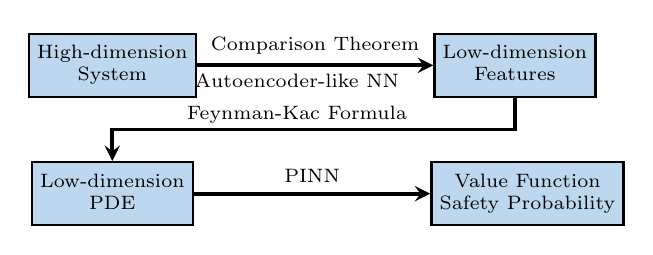
\begin{tikzpicture}[
    node distance = 4cm,
    node/.style={circle, fill=#1, inner sep=2pt, minimum size=0.7cm}, 
    edge/.style={-stealth, #1}
]

% 
\node[rectangle, draw=black, fill = newblue,line width = 0.3mm, minimum height=0.8cm,minimum width=2cm,inner sep=-3pt] (hds){\scriptsize \begin{tabular}{cc}
High-dimension \\ System
\end{tabular}};

\node[rectangle, draw=black, fill = newblue,line width = 0.3mm, minimum height=0.8cm,minimum width=2cm,inner sep=-3pt][right = 3cm of hds] (ldf){\scriptsize \begin{tabular}{cc}
Low-dimension \\ Features
\end{tabular}};


\node[rectangle, draw=black, fill = newblue,line width = 0.3mm, minimum height=0.8cm,minimum width=2cm,inner sep=-3pt][below = 0.8cm of hds] (pde){\scriptsize \begin{tabular}{cc}
Low-dimension \\ PDE
\end{tabular}};

\node[rectangle, draw=black, fill = newblue,line width = 0.3mm, minimum height=0.8cm,minimum width=2cm,inner sep=-3pt][right = 3cm of pde] (vfsp){\scriptsize \begin{tabular}{cc}
Value Function \\ Safety Probability
\end{tabular}};


%Edges
% \draw[edge=black,line width = 0.5mm] (hds) -> (pdf);

\draw [edge=black,line width = 0.5mm] (hds) -- (ldf) node[midway,above] {\scriptsize Comparison Theorem};

\node[rectangle][above left= -0.9cm and 0.1cm of ldf] (ct){\scriptsize \begin{tabular}{cc}
\color{black}{Autoencoder-like NN}
\end{tabular}};

% \draw [edge=black,line width = 0.3mm] (pdf) -- (pde) node[midway,above] {\scriptsize Comparison theorem};
\draw [edge=black,line width = 0.5mm, draw] (ldf.south) -- ++(0,-0.4) node(midway, north){} -| (pde.north);

\node[rectangle][below left= -0.05cm and 0cm of ldf] (ct){\scriptsize \begin{tabular}{cc}
\color{black}{Feynman-Kac Formula}
\end{tabular}};

% \node[rectangle][below left= 0.28cm and -0.5cm of pdf] (ct){\scriptsize \begin{tabular}{cc}
% \color{black}{Feynman-Kac Lemma}
% \end{tabular}};

\draw [edge=black,line width = 0.5mm] (pde) -- (vfsp) node[midway, above] {\scriptsize PINN};

\end{tikzpicture}
    \caption{The procedure diagram of the proposed method.}
    \label{fig:flowchart}
\end{figure}

% \vspace{-1em}

\subsection{Comparison Theorem for Feature Identification}
We assume the low-dimensional feature can be represented by a smooth function $p: \mathbb{R}^n \rightarrow \mathbb{R}$. Here, we use comparison theorem~\cite[Theorem 3.1]{ikeda1977comparison} to find the stochastic process $\xi$ that describes the exact evolution of $p(x)$.
% for the uncontrolled system~\eqref{eq:continuous_dynamics} with $u \equiv 0$.
We introduce the operator $\mathcal{A}$ as
% \begin{equation}
% \label{eq:def_L}
%     \mathcal{L}^U(\cdot)=\frac{\partial(\cdot)}{\partial x} f(x)+\frac{\partial(\cdot)}{\partial x} \sigma(x) U+\frac{1}{2} \operatorname{Tr}\left(\frac{\partial^2(\cdot)}{\partial x^2}(x) \sigma(x) \sigma(x)^T\right)
% \end{equation}
\begin{equation}
\label{eq:def_L}
\begin{aligned}
\mathcal{A}^U(\cdot)(x) & =\frac{\partial(\cdot)}{\partial x}(x) f(x)+ \frac{\partial (\cdot)}{\partial x}(x) \sigma(x) U + \\
& \qquad \frac{1}{2} \operatorname{Tr}\left(\frac{\partial^2(\cdot)}{\partial x^2}(x) \sigma(x) \sigma(x)^\top\right),
\end{aligned}
\end{equation}
where $U: \mathbb{R}^n \rightarrow \mathbb{R}^m$ is the control policy that maps the state to the control input, and we define
\begin{equation}
    a(x)=\sum_{i, j, k} \sigma_k^i(x) \sigma_k^j(x) \frac{\partial p}{\partial x_i}(x) \frac{\partial p}{\partial x_j}(x), \; b(x)=\frac{\mathcal{A}^U p(x)}{a(x)},
\end{equation}
where $\sigma_k^i(x)$ is the $(i,k)$-th element of the diffusion coefficient $\sigma(x)$.
For value function estimation, we consider $\mathcal{A}^0$ for the uncontrolled process where $U \equiv 0$, and for safety probability estimation, we consider $\mathcal{A}^{\mathcal{N}}$ where $U = \mathcal{N}$ is the nominal control policy.
% $\mathcal{L}^0$ is the operator~\eqref{eq:def_L} with $U \equiv 0$. 
Additionally, let $\xi \in I \subset \mathbb{R}$ be a scalar variable, where $I$ is the range of the feature $p(x)$. Using similar notation employed in~\cite{ikeda1977comparison}, consider
\begin{equation}
\label{eq:a_b_def}
\begin{aligned}
    a^{+}(\xi) = \sup _{x: p(x)=\xi} a(x), & \quad a^{-}(\xi) = \inf _{x: p(x)=\xi} a(x) \\
    b^{+}(\xi)= \sup _{x: p(x)=\xi} b(x), & \quad b^{-}(\xi)=\inf _{x: p(x)=\xi} b(x)
\end{aligned}
\end{equation}
\begin{assumption}
\label{asm:match_upper_lower_bound}
We assume that the feature function $p(x)$ satisfies that $a^{+}(\xi) = a^{-}(\xi) = \alpha(\xi)$ and $b^{+}(\xi) = b^{-}(\xi) = \beta(\xi)$, $\forall \xi \in I$. 
\end{assumption}
\begin{assumption}
\label{asm:continuity-condition-on-a-and-b}
The functions $\alpha(\xi)$ and $\beta(\xi)$ are globally Lipschitz continuous in $\xi \in I \subset \mathbb{R}$.
Moreover, $a(x) > 0$, $\forall x \in \mathbb{R}^{n}$.
\end{assumption}
% \jacob{add explanations to the assumptions}

\begin{theorem}
\label{thm:comparison_lemma}
Given Assumptions~\ref{asm:match_upper_lower_bound} and~\ref{asm:continuity-condition-on-a-and-b} hold, $p(x_t)$ with $x_t$ being sampled from system~\eqref{eq:continuous_dynamics} is characterized by the following stochastic process
\begin{equation}
\label{eq:one_dim_xi_process}
    d \xi_t = \alpha\left(\xi_t\right) \beta\left(\xi_t\right) d t + \sqrt{\alpha\left(\xi_t\right)} d \tilde{B}_t,
\end{equation}
with $\xi_0 = p(x_0)$, and $\tilde{B}_t$ being a one-dimensional standard Wiener process.
\end{theorem}
\begin{proof}
    % See extended version of the paper~\cite{}. \todo{}
    See appendix.
\end{proof}
% Given Assumptions~\ref{asm:match_upper_lower_bound} and~\ref{asm:continuity-condition-on-a-and-b} hold, from~\cite[Theorem 3.1]{ikeda1977comparison} we know that $p(x_t)$ with $x_t$ being sampled from system~\eqref{eq:continuous_dynamics}, is characterized by the following process
% \begin{equation}
% \label{eq:one_dim_xi_process}
%     d \xi_t = \alpha\left(\xi_t\right) \beta\left(\xi_t\right) d t + \sqrt{\alpha\left(\xi_t\right)} d \tilde{B}_t,
% \end{equation}
% with $\xi_0 = p(x_0)$, and $\tilde{B}_t$ being a one-dimensional standard Wiener process.
Assumption~\ref{asm:match_upper_lower_bound} gives the conditions for the upper and lower bounds to match with the actual value $\alpha$ and $\beta$, thus a single stochastic process $\xi$ can be derived.
Till here, we have found the one-dimensional process~\eqref{eq:one_dim_xi_process} that characterizes the evolution of the feature of the high-dimensional system.

\subsection{PDE for Value Function with Feynman-Kac}
\label{sec:Feynman_Kac_PDE}
In this section, we describe how to estimate the value function with the solution of a low-dimensional PDE.
We consider $p(x) = c(x)$, \ie the feature of the high-dimensional system is the value of the running cost on state.
We set
\begin{equation}
\label{eq:V_exp_transformation}
    V(x, t)=-\log \varphi(x, t).
\end{equation}
Let $\xi = p(x)$, then from~\eqref{eq:value_function_free_energy} we have
\begin{equation}
\label{eq:xi_value_function}
\begin{aligned}
    \varphi(x, t) %& = \mathbb{E} \left[\exp \left(-\int_t^T c\left(x_\tau\right) d \tau - c(x_T)\right)  \mid x_t=x\right] \\
    & = \mathbb{E} \left[\exp \left(-\int_t^T \xi_\tau d \tau - \xi_T\right)  \mid \xi_t=\xi\right] 
\end{aligned}
\end{equation}
With that, we apply Feynman-Kac formula~\cite{del2004feynman} on~\eqref{eq:xi_value_function} and~\eqref{eq:one_dim_xi_process} and get $\varphi(x, t)$ is the solution of the following two-dimensional PDE
\begin{equation}
\label{eq:one_dim_PDE}
\begin{aligned}
    W_{\varphi}(\xi,t) := & \frac{\partial \varphi}{\partial t}(\xi, t) + \alpha(\xi, t)\beta(\xi, t)\frac{\partial \varphi}{\partial \xi}(\xi, t) \\
    & +\frac{1}{2} \alpha(\xi, t) \frac{\partial^2 \varphi}{\partial \xi^2}(\xi, t) - \xi \varphi(\xi, t)=0,
\end{aligned}
\end{equation}
with initial (terminal) condition
\begin{equation}
\label{eq:one_dim_PDE_ic}
    \varphi(\xi, T) = \exp(-\frac{1}{2}\xi).
\end{equation}
%This is a 2-dimensional PDE that has no boundary conditions, and can be efficiently solved using a PINN. Here, we use $W_{\varphi}$ to denote the actual value of the PDE~\eqref{eq:one_dim_PDE} given $\varphi$ to better define the loss function in the PINN.
% \begin{remark}
%     The reason we consider the exponential transformation~\eqref{eq:V_exp_transformation} is that
% \end{remark}

\subsection{PDE for Safety Probability}
In this section, we describe how to estimate the safety probability with the solution of a low-dimensional PDE. We consider $p(x) = \phi(x)$, \ie the feature of the high-dimensional system is the value of the barrier function for the state. Then we have
\begin{equation}
\label{eq:safety_prob_hitting_time}
\begin{aligned}
    & \quad F(x,t) = \pr\left(x_\tau \in \safe, \forall \tau\in [0,t] \mid x_0 =x \right) \\
    & = \pr\left(\min_{0\leq \tau \leq t} \phi(x_\tau) \geq 0\right) = \pr\left(\min_{0\leq \tau \leq t} p(x_\tau) \geq 0\right) \\
    & = \pr\left(\min_{0\leq \tau \leq t} \xi_\tau \geq 0\right).
\end{aligned}
\end{equation}
The well-known results on the probability distribution of the first hitting time~\cite{patie2008first} allow us to obtain~\eqref{eq:safety_prob_hitting_time} as a solution to the two-dimensional PDE given by
\begin{equation}
\label{eq:one_dim_PDE_safe_prob}
\begin{aligned}
    W_{F}(\xi,t) := & \frac{\partial F}{\partial t}(\xi, t) - \alpha(\xi, t)\beta(\xi, t)\frac{\partial F}{\partial \xi}(\xi, t) \\
    & \quad - \frac{1}{2} \alpha(\xi, t) \frac{\partial^2 F}{\partial \xi^2}(\xi, t) =0,
\end{aligned}
\end{equation}
with boundary and initial conditions
\begin{equation}\label{eq:safe_PDE_ic_bc}
      F(\xi, 0)  = 1, \,\, \xi > 0; \quad F(0, t)  = 0, \,\, t > 0.
\end{equation}
  
%This is a 2-dimensional PDE that can be solved efficiently with a PINN . We use $W_{F}$ to denote the actual value of the PDE~\eqref{eq:one_dim_PDE_safe_prob} given $F$.


\subsection{Physic-informed Learning}
% \todo{change the narritive to account for both value function and safety probability}

In this section, we will introduce a physics-informed learning pipeline to solve the PDE for the value function~\eqref{eq:one_dim_PDE} and the PDE for safety probability~\eqref{eq:one_dim_PDE_safe_prob}. For conciseness, we will focus on the case of value function estimation, as adaptation to safety probability estimation is trivial where one just need to replace the variables and the governing PDE.

From~\eqref{eq:path_integral_MC_estimation}, we can estimate the value function using path integral control by sampling the uncontrolled process. However, the path integral MC is not sample efficient when we want to know the value function on the entire space, especially for a large horizon $T$. Further, efficiently solving the value function PDE~\eqref{eq:one_dim_PDE} using standard numerical methods is challenging. 

To leverage the advantages of MC and PDE methods and to overcome their drawbacks, we propose a physics-informed neural network (PINN) to learn the mapping from the feature-time pair to the value function $\varphi$.
Fig.~\ref{fig:PINN diagram} shows the architecture of the PINN. The PINN takes the feature-time pair $(\xi,t)$ as the input, and outputs the value function prediction $\hat{\varphi}$, the feature and time derivatives $ \frac{\partial \hat \varphi}{\partial \xi}$ and $ \frac{\partial \hat \varphi}{\partial t}$, and the Hessian $ \frac{\partial^2 \hat \varphi}{\partial \xi^2}$, which come naturally from the automatic differentiation in deep learning frameworks such as PyTorch~\cite{paszke2019pytorch} and TensorFlow~\cite{abadi2016tensorflow}.
Assume the PINN is parameterized by $\boldsymbol\theta$, the loss function is defined as
\begin{equation}
\label{eq:PINN overall loss function}
    \mathcal{L}(\boldsymbol\theta) = \omega_p \mathcal{L}_p(\boldsymbol\theta) + \omega_d \mathcal{L}_d(\boldsymbol\theta),
\end{equation}
where
\begin{equation}
\label{eq:PINN loss functions}
\begin{aligned}
    \mathcal{L}_p(\boldsymbol\theta) & = \frac{1}{|\mathcal{P}|} \sum_{(\xi,t) \in \mathcal{P}} \|W_{\hat{\varphi}_{\boldsymbol\theta}}(\xi,t)\|_2^2, \\
    \mathcal{L}_d(\boldsymbol\theta) & = \frac{1}{|\mathcal{D}|} \sum_{(\xi,t) \in \mathcal{D}} \|\hat{\varphi}_{\boldsymbol\theta}(\xi,t) - \bar{\varphi}(\xi,t)\|_2^2.
\end{aligned}
\end{equation}
Here, $\bar{\varphi}$ is the training data, $\hat{\varphi}_{\boldsymbol\theta}$ is the prediction from the PINN, $\mathcal{P}$ and $\mathcal{D}$ are the training point sets for the physics model and external data, respectively. The loss function $\mathcal{L}$ consists of two parts, the physics model loss $\mathcal{L}_p$ and data loss $\mathcal{L}_d$. The physics model loss $\mathcal{L}_p$ measures the satisfaction of the PDE constraints for the learned output. It calculates the actual PDE equation value $W_{\hat{\varphi}_{\boldsymbol\theta}}$, which is supposed to be $0$, and use its 2-norm as the loss. The data loss $\mathcal{L}_d$ measures the accuracy of the prediction of PINN on the training data. It calculates the mean square error between the PINN prediction and the training data point as the loss. The overall loss function $\mathcal{L}$ is the weighted sum of the physics model loss and data loss with weighting coefficients $\omega_p$ and $\omega_d$.
Though out of the scope of this paper, theoretical analysis on the approximation error of PINNs and neural operators can be found in~\cite{wang2023generalizable, lu2021learning, kovachki2021universal}. 
% \todo{review this part and the remark below}
% \begin{figure*}[t]
%     \centering
%     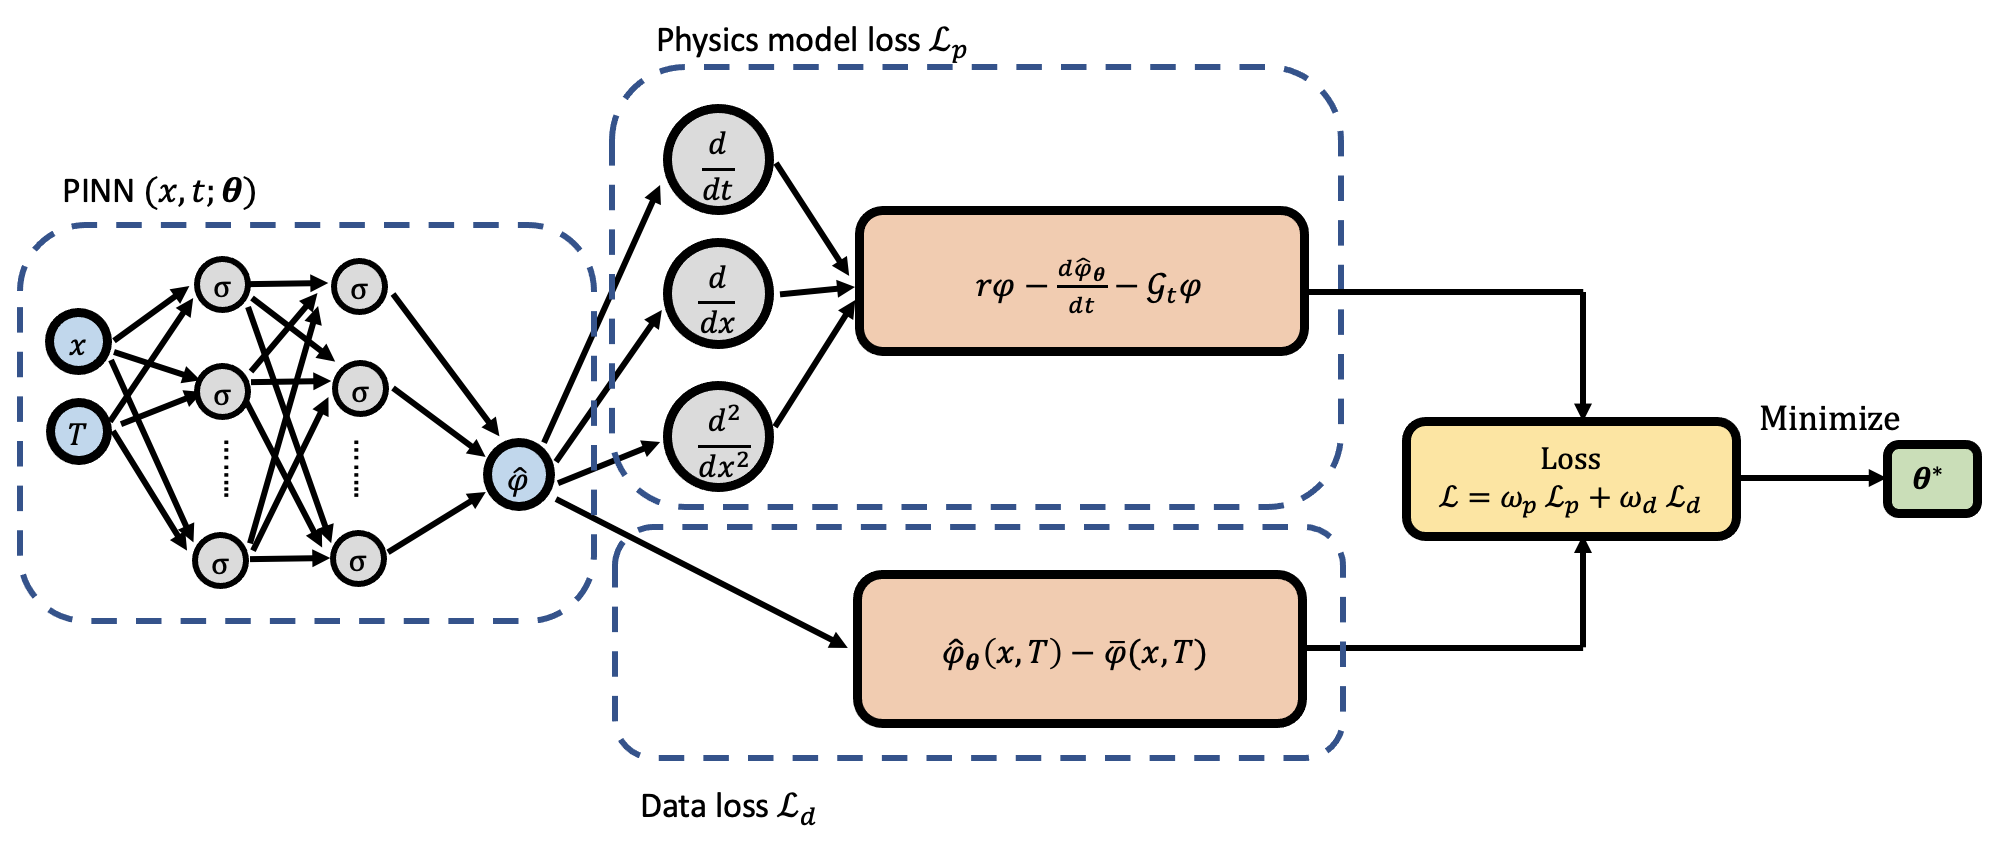
\includegraphics[width=13cm]{Figures/PINN_diagram.png}
%     \caption{The training scheme of the physics-informed neural network (PINN). \todo{maybe add the safety probability version in the same plot?}
%     }
%     \label{fig:PINN diagram}
% \end{figure*}

\begin{figure*}[t]
\begin{subfigure}[t]{0.65\textwidth}
\centering
\tikzstyle{line} = [draw, -latex']

\tikzset{
diagonal fill/.style 2 args={fill=#2, path picture={
\fill[#1, sharp corners] (path picture bounding box.south west) -|
                         (path picture bounding box.north east) -- cycle;}},
reversed diagonal fill/.style 2 args={fill=#2, path picture={
\fill[#1, sharp corners] (path picture bounding box.north west) |- 
                         (path picture bounding box.south east) -- cycle;}}
}

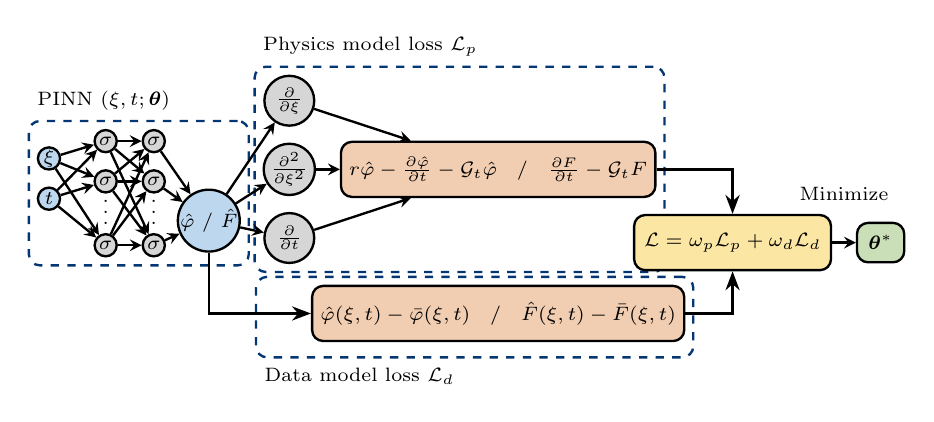
\begin{tikzpicture}[
    node distance = 1.2cm,
    fontscale/.style = {font=\scriptsize},
    node/.style={circle, fill=#1, inner sep=0pt, minimum size=0.1cm}, 
    edge/.style={-stealth, #1},
    arr/.style = {semithick, -Stealth}
]
    
    %Block 1
    %Nodes
    \node[circle, fill = newblue, draw=black, line width=0.3mm, inner sep=0pt, minimum size=8pt]  (xi) {\scriptsize $\xi$};
    \node[circle, fill = newblue, draw=black, line width=0.3mm, inner sep=0pt, minimum size=8pt] (t) [below = 0.2cm of xi] {\scriptsize $t$};

    \node[circle, fill = newgray, draw=black, line width=0.3mm, inner sep=0pt, minimum size=8pt]  (sigma1)[above right = -0cm and 0.5cm of xi] {\scriptsize $\sigma$};
    \node[circle, fill = newgray, draw=black, line width=0.3mm, inner sep=0pt, minimum size=8pt]  (sigma2)[below = 0.2cm of sigma1] {\scriptsize $\sigma$};
    \node[circle, fill = newgray, draw=black, line width=0.3mm, inner sep=0pt, minimum size=8pt]  (sigma3)[below = 0.5cm of sigma2] {\scriptsize $\sigma$};

    \node[circle, fill = newgray, draw=black, line width=0.3mm, inner sep=0pt, minimum size=8pt]  (sigma4)[right = 0.3cm of sigma1] {\scriptsize $\sigma$};
    \node[circle, fill = newgray, draw=black, line width=0.3mm, inner sep=0pt, minimum size=8pt]  (sigma5)[right = 0.3cm of sigma2] {\scriptsize $\sigma$};
    \node[circle, fill = newgray, draw=black, line width=0.3mm, inner sep=0pt, minimum size=8pt]  (sigma6)[right = 0.3cm of sigma3] {\scriptsize $\sigma$};

    \node[circle, fill = newblue, draw=black, line width=0.3mm, inner sep=0pt, minimum size=8pt]  (phi)[below right = 0.1cm and 0.3cm of sigma5] {\scriptsize $\hat \varphi$ / $\hat F$};


    %Edges
    % \draw[edge=blue,line width=0.5mm] (A) ->node[above]{$p$} (B);
    \draw[edge,line width=0.3mm] (xi) -> (sigma1);
    \draw[edge,line width=0.3mm] (xi) -> (sigma2);
    \draw[edge,line width=0.3mm] (xi) -> (sigma3);

    \draw[edge,line width=0.3mm] (t) -> (sigma1);
    \draw[edge,line width=0.3mm] (t) -> (sigma2);
    \draw[edge,line width=0.3mm] (t) -> (sigma3);

    \draw[edge,line width=0.3mm] (sigma1) -> (sigma4);
    \draw[edge,line width=0.3mm] (sigma1) -> (sigma5);
    \draw[edge,line width=0.3mm] (sigma1) -> (sigma6);

    \draw[edge,line width=0.3mm] (sigma2) -> (sigma4);
    \draw[edge,line width=0.3mm] (sigma2) -> (sigma5);
    \draw[edge,line width=0.3mm] (sigma2) -> (sigma6);

    \draw[edge,line width=0.3mm] (sigma3) -> (sigma4);
    \draw[edge,line width=0.3mm] (sigma3) -> (sigma5);
    \draw[edge,line width=0.3mm] (sigma3) -> (sigma6);

    \node at ($(sigma2)!.35!(sigma3)$) {\scriptsize \vdots};
    \node at ($(sigma5)!.35!(sigma6)$) {\scriptsize \vdots};

    \draw[edge,line width=0.3mm] (sigma4) -> (phi);
    \draw[edge,line width=0.3mm] (sigma5) -> (phi);
    \draw[edge,line width=0.3mm] (sigma6) -> (phi);

    \node[rectangle, draw=cmublue, fit=(xi) (sigma1) (sigma3) (phi), rounded corners, dashed, line width=0.3mm, inner sep=1mm] (block1) {};
    \node[above right] at (block1.north west){\scriptsize PINN $(\xi,t;\boldsymbol\theta)$};

    

    % block2
    \node[circle, fill = newgray, draw=black, line width=0.3mm, inner sep=0pt, minimum size=18pt]  (par1)[above right= 1cm and 0.5cm of phi] {\scriptsize $\frac{\partial}{\partial\xi}$};
    \node[circle, fill = newgray, draw=black, line width=0.3mm, inner sep=0pt, minimum size=18pt]  (par2)[below= 0.2cm of par1] {\scriptsize $\frac{\partial^2}{\partial\xi^2}$};
PF    \node[circle, fill = newgray, draw=black, line width=0.3mm, inner sep=0pt, minimum size=18pt]  (par3)[below= 0.2cm of par2] {\scriptsize $\frac{\partial}{\partial t}$};

    \node[rectangle, fill = neworange, draw=black, line width=0.3mm, inner sep=3pt, minimum height = 0.7cm, minimum width = 2.5cm, rounded corners]  (eq1)[right= 0.3cm of par2] {\scriptsize $r \hat \varphi -\frac{\partial \hat \varphi}{\partial t}-\mathcal{G}_t \hat \varphi$ \: / \: $\frac{\partial F}{\partial t}-\mathcal{G}_t F$};

    \draw[edge,line width=0.3mm] (par1) -> (eq1);
    \draw[edge,line width=0.3mm] (par2) -> (eq1);
    \draw[edge,line width=0.3mm] (par3) -> (eq1);

    \node[rectangle, draw=cmublue, fit=(par1) (par2) (par3) (eq1), rounded corners, dashed, line width=0.3mm, inner sep=1mm] (block2) {};
    \node[above right] at (block2.north west){\scriptsize Physics model loss $\mathcal{L}_p$};

    % block3
    \node[rectangle, fill = neworange, draw=black, line width=0.3mm, inner sep=3pt, minimum height = 0.7cm, minimum width = 2.5cm, rounded corners] (eq2)[below= 1.1cm of eq1] {\scriptsize $\hat{\varphi}(\xi,t) - \bar{\varphi}(\xi,t)$ \: / \: $\hat{F}(\xi,t) - \bar{F}(\xi,t)$};
    \node[circle, inner sep=0pt, minimum size=18pt] (par4)[below= 1.3cm of par2] {};
    \node[rectangle, draw=cmublue, fit=(par4) (eq2), rounded corners, dashed, line width=0.3mm, inner sep=1mm] (block3) {};
    \node[below right] at (block3.south west){\scriptsize Data model loss $\mathcal{L}_d$};

    
    \draw[edge,line width=0.3mm] (phi) -> (par1);
    \draw[edge,line width=0.3mm] (phi) -> (par2);
    \draw[edge,line width=0.3mm] (phi) -> (par3);
    % \draw[edge,line width=0.3mm] (phi) -> (eq2);
    \draw [arr,line width=0.3mm] (phi) |- (eq2);

    % loss
    \node[rectangle, fill = newyellow, draw=black, line width=0.3mm, inner sep=0pt, minimum height = 0.7cm, minimum width = 2.5cm, rounded corners]  (loss)[below right= 0.2cm and -0.3cm of eq1] {\scriptsize  $\mathcal{L} = \omega_p \mathcal{L}_p + \omega_d \mathcal{L}_d$};
    \draw [arr,line width=0.3mm] (eq1) -| (loss);
    \draw [arr,line width=0.3mm] (eq2) -| (loss);

    % theta
    \node[rectangle, fill = newgreen, draw=black, line width=0.3mm, inner sep=0pt, minimum height = 0.5cm, minimum width = 0.6cm, rounded corners]  (theta)[right= 0.3cm of loss] {\scriptsize $\boldsymbol\theta^*$};
    % \draw[edge,line width=0.3mm, label = minimize] (loss) -> (theta);
    \path[-stealth,draw,line width=0.3mm](loss) edge node[above=0.4cm] {\scriptsize Minimize} (theta);
    

\end{tikzpicture}

 
\phantomsubcaption
\label{fig:PINN diagram}
\end{subfigure}
\hfill
\begin{subfigure}[t]{0.35\textwidth}
\centering
\phantomsubcaption
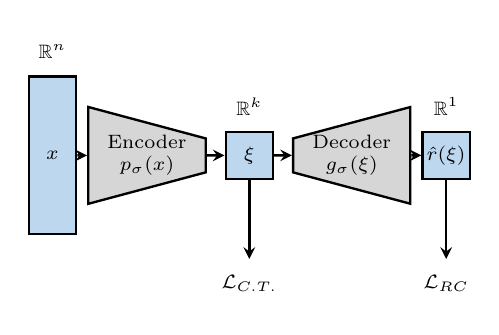
\begin{tikzpicture}[
    node distance = 4cm,
    node/.style={circle, fill=#1, inner sep=2pt, minimum size=0.7cm}, 
    edge/.style={-stealth, #1}
]

% x
\node[rectangle, draw, line width=0.3mm, fill = newblue, minimum height=2cm,minimum width=0.6cm,inner sep=0pt] at (0,0) (x){\scriptsize $x$};

\node[rectangle, minimum height=0.6cm,minimum width=0.6cm,inner sep=0pt] (r1)[above = 0cm of x]{\scriptsize $\mathbb{R}^n$};

% encoder
\node[trapezium,draw,line width=0.3mm,trapezium angle=75, minimum width = 1.23cm, fill = newgray, 
    minimum height = 1.3cm, rotate = -90, inner sep = -3pt](encoder)at (1.2,0) {\scriptsize \rotatebox{90}{\begin{tabular}{cc} Encoder \\ $p_\sigma (x)$ \end{tabular}}};

% xi
\node[rectangle, draw, line width=0.3mm, fill = newblue, minimum height=0.6cm,minimum width=0.6cm,inner sep=0pt] at (2.5,0) (xi){\scriptsize $\xi$};

\node[rectangle, minimum height=0.6cm,minimum width=0.6cm,inner sep=0pt] (r2)[above = 0cm of xi]{\scriptsize $\mathbb{R}^k$};

\node[rectangle, minimum height=0.6cm,minimum width=0.6cm,inner sep=0pt] (l1)[below = 1cm of xi]{\scriptsize $\mathcal{L}_{C.T.}$};

% decoder
\node[trapezium,draw,line width=0.3mm,trapezium angle=75, minimum width = 1.23cm, fill = newgray, 
    minimum height = 1.3cm, rotate = 90, inner sep = -3pt](decoder)at (3.8,0) {\scriptsize \rotatebox{-90}{\begin{tabular}{cc} Decoder \\ $g_\sigma (\xi)$ \end{tabular}}};

% g
\node[rectangle, draw, line width=0.3mm, fill = newblue, minimum height=0.6cm, minimum width=0.6cm,inner sep=0pt] at (5,0) (f){\scriptsize $\hat{r}(\xi)$};

\node[rectangle, minimum height=0.6cm,minimum width=0.6cm,inner sep=0pt] (r3)[above = 0cm of f]{\scriptsize $\mathbb{R}^1$};

\node[rectangle, minimum height=0.6cm,minimum width=0.6cm,inner sep=0pt] (l2)[below = 1cm of f]{\scriptsize $\mathcal{L}_{RC}$};

% arrows
\draw[edge,line width=0.3mm] (x) -> (encoder);
\draw[edge,line width=0.3mm] (encoder) -> (xi);
\draw[edge,line width=0.3mm] (xi) -> (decoder);
\draw[edge,line width=0.3mm] (decoder) -> (f);
\draw[edge,line width=0.3mm] (xi) -> (l1);
\draw[edge,line width=0.3mm] (f) -> (l2);
\end{tikzpicture}
\label{fig:AE diagram}
\end{subfigure}
\caption{(\subref{fig:PINN diagram}) The training scheme of the physics-informed neural network (PINN).
        (\subref{fig:AE diagram}) Autoencoder-like network architecture.}
\end{figure*}

% \begin{figure*}[t]
%     \centering  {(a)~\tikzstyle{line} = [draw, -latex']

\tikzset{
diagonal fill/.style 2 args={fill=#2, path picture={
\fill[#1, sharp corners] (path picture bounding box.south west) -|
                         (path picture bounding box.north east) -- cycle;}},
reversed diagonal fill/.style 2 args={fill=#2, path picture={
\fill[#1, sharp corners] (path picture bounding box.north west) |- 
                         (path picture bounding box.south east) -- cycle;}}
}

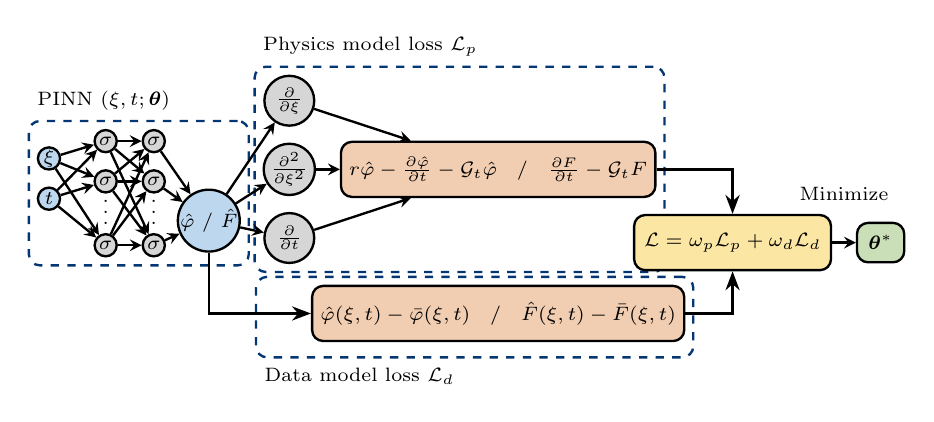
\begin{tikzpicture}[
    node distance = 1.2cm,
    fontscale/.style = {font=\scriptsize},
    node/.style={circle, fill=#1, inner sep=0pt, minimum size=0.1cm}, 
    edge/.style={-stealth, #1},
    arr/.style = {semithick, -Stealth}
]
    
    %Block 1
    %Nodes
    \node[circle, fill = newblue, draw=black, line width=0.3mm, inner sep=0pt, minimum size=8pt]  (xi) {\scriptsize $\xi$};
    \node[circle, fill = newblue, draw=black, line width=0.3mm, inner sep=0pt, minimum size=8pt] (t) [below = 0.2cm of xi] {\scriptsize $t$};

    \node[circle, fill = newgray, draw=black, line width=0.3mm, inner sep=0pt, minimum size=8pt]  (sigma1)[above right = -0cm and 0.5cm of xi] {\scriptsize $\sigma$};
    \node[circle, fill = newgray, draw=black, line width=0.3mm, inner sep=0pt, minimum size=8pt]  (sigma2)[below = 0.2cm of sigma1] {\scriptsize $\sigma$};
    \node[circle, fill = newgray, draw=black, line width=0.3mm, inner sep=0pt, minimum size=8pt]  (sigma3)[below = 0.5cm of sigma2] {\scriptsize $\sigma$};

    \node[circle, fill = newgray, draw=black, line width=0.3mm, inner sep=0pt, minimum size=8pt]  (sigma4)[right = 0.3cm of sigma1] {\scriptsize $\sigma$};
    \node[circle, fill = newgray, draw=black, line width=0.3mm, inner sep=0pt, minimum size=8pt]  (sigma5)[right = 0.3cm of sigma2] {\scriptsize $\sigma$};
    \node[circle, fill = newgray, draw=black, line width=0.3mm, inner sep=0pt, minimum size=8pt]  (sigma6)[right = 0.3cm of sigma3] {\scriptsize $\sigma$};

    \node[circle, fill = newblue, draw=black, line width=0.3mm, inner sep=0pt, minimum size=8pt]  (phi)[below right = 0.1cm and 0.3cm of sigma5] {\scriptsize $\hat \varphi$ / $\hat F$};


    %Edges
    % \draw[edge=blue,line width=0.5mm] (A) ->node[above]{$p$} (B);
    \draw[edge,line width=0.3mm] (xi) -> (sigma1);
    \draw[edge,line width=0.3mm] (xi) -> (sigma2);
    \draw[edge,line width=0.3mm] (xi) -> (sigma3);

    \draw[edge,line width=0.3mm] (t) -> (sigma1);
    \draw[edge,line width=0.3mm] (t) -> (sigma2);
    \draw[edge,line width=0.3mm] (t) -> (sigma3);

    \draw[edge,line width=0.3mm] (sigma1) -> (sigma4);
    \draw[edge,line width=0.3mm] (sigma1) -> (sigma5);
    \draw[edge,line width=0.3mm] (sigma1) -> (sigma6);

    \draw[edge,line width=0.3mm] (sigma2) -> (sigma4);
    \draw[edge,line width=0.3mm] (sigma2) -> (sigma5);
    \draw[edge,line width=0.3mm] (sigma2) -> (sigma6);

    \draw[edge,line width=0.3mm] (sigma3) -> (sigma4);
    \draw[edge,line width=0.3mm] (sigma3) -> (sigma5);
    \draw[edge,line width=0.3mm] (sigma3) -> (sigma6);

    \node at ($(sigma2)!.35!(sigma3)$) {\scriptsize \vdots};
    \node at ($(sigma5)!.35!(sigma6)$) {\scriptsize \vdots};

    \draw[edge,line width=0.3mm] (sigma4) -> (phi);
    \draw[edge,line width=0.3mm] (sigma5) -> (phi);
    \draw[edge,line width=0.3mm] (sigma6) -> (phi);

    \node[rectangle, draw=cmublue, fit=(xi) (sigma1) (sigma3) (phi), rounded corners, dashed, line width=0.3mm, inner sep=1mm] (block1) {};
    \node[above right] at (block1.north west){\scriptsize PINN $(\xi,t;\boldsymbol\theta)$};

    

    % block2
    \node[circle, fill = newgray, draw=black, line width=0.3mm, inner sep=0pt, minimum size=18pt]  (par1)[above right= 1cm and 0.5cm of phi] {\scriptsize $\frac{\partial}{\partial\xi}$};
    \node[circle, fill = newgray, draw=black, line width=0.3mm, inner sep=0pt, minimum size=18pt]  (par2)[below= 0.2cm of par1] {\scriptsize $\frac{\partial^2}{\partial\xi^2}$};
PF    \node[circle, fill = newgray, draw=black, line width=0.3mm, inner sep=0pt, minimum size=18pt]  (par3)[below= 0.2cm of par2] {\scriptsize $\frac{\partial}{\partial t}$};

    \node[rectangle, fill = neworange, draw=black, line width=0.3mm, inner sep=3pt, minimum height = 0.7cm, minimum width = 2.5cm, rounded corners]  (eq1)[right= 0.3cm of par2] {\scriptsize $r \hat \varphi -\frac{\partial \hat \varphi}{\partial t}-\mathcal{G}_t \hat \varphi$ \: / \: $\frac{\partial F}{\partial t}-\mathcal{G}_t F$};

    \draw[edge,line width=0.3mm] (par1) -> (eq1);
    \draw[edge,line width=0.3mm] (par2) -> (eq1);
    \draw[edge,line width=0.3mm] (par3) -> (eq1);

    \node[rectangle, draw=cmublue, fit=(par1) (par2) (par3) (eq1), rounded corners, dashed, line width=0.3mm, inner sep=1mm] (block2) {};
    \node[above right] at (block2.north west){\scriptsize Physics model loss $\mathcal{L}_p$};

    % block3
    \node[rectangle, fill = neworange, draw=black, line width=0.3mm, inner sep=3pt, minimum height = 0.7cm, minimum width = 2.5cm, rounded corners] (eq2)[below= 1.1cm of eq1] {\scriptsize $\hat{\varphi}(\xi,t) - \bar{\varphi}(\xi,t)$ \: / \: $\hat{F}(\xi,t) - \bar{F}(\xi,t)$};
    \node[circle, inner sep=0pt, minimum size=18pt] (par4)[below= 1.3cm of par2] {};
    \node[rectangle, draw=cmublue, fit=(par4) (eq2), rounded corners, dashed, line width=0.3mm, inner sep=1mm] (block3) {};
    \node[below right] at (block3.south west){\scriptsize Data model loss $\mathcal{L}_d$};

    
    \draw[edge,line width=0.3mm] (phi) -> (par1);
    \draw[edge,line width=0.3mm] (phi) -> (par2);
    \draw[edge,line width=0.3mm] (phi) -> (par3);
    % \draw[edge,line width=0.3mm] (phi) -> (eq2);
    \draw [arr,line width=0.3mm] (phi) |- (eq2);

    % loss
    \node[rectangle, fill = newyellow, draw=black, line width=0.3mm, inner sep=0pt, minimum height = 0.7cm, minimum width = 2.5cm, rounded corners]  (loss)[below right= 0.2cm and -0.3cm of eq1] {\scriptsize  $\mathcal{L} = \omega_p \mathcal{L}_p + \omega_d \mathcal{L}_d$};
    \draw [arr,line width=0.3mm] (eq1) -| (loss);
    \draw [arr,line width=0.3mm] (eq2) -| (loss);

    % theta
    \node[rectangle, fill = newgreen, draw=black, line width=0.3mm, inner sep=0pt, minimum height = 0.5cm, minimum width = 0.6cm, rounded corners]  (theta)[right= 0.3cm of loss] {\scriptsize $\boldsymbol\theta^*$};
    % \draw[edge,line width=0.3mm, label = minimize] (loss) -> (theta);
    \path[-stealth,draw,line width=0.3mm](loss) edge node[above=0.4cm] {\scriptsize Minimize} (theta);
    

\end{tikzpicture}

 \phantomsubcaption\label{fig:PINN diagram}}
%     {(b)~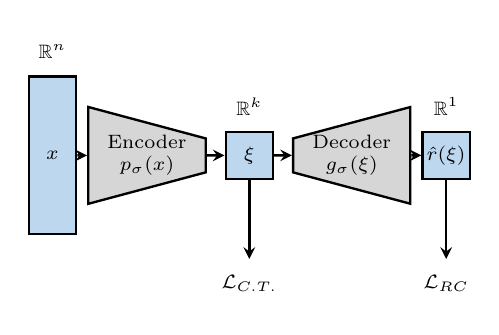
\begin{tikzpicture}[
    node distance = 4cm,
    node/.style={circle, fill=#1, inner sep=2pt, minimum size=0.7cm}, 
    edge/.style={-stealth, #1}
]

% x
\node[rectangle, draw, line width=0.3mm, fill = newblue, minimum height=2cm,minimum width=0.6cm,inner sep=0pt] at (0,0) (x){\scriptsize $x$};

\node[rectangle, minimum height=0.6cm,minimum width=0.6cm,inner sep=0pt] (r1)[above = 0cm of x]{\scriptsize $\mathbb{R}^n$};

% encoder
\node[trapezium,draw,line width=0.3mm,trapezium angle=75, minimum width = 1.23cm, fill = newgray, 
    minimum height = 1.3cm, rotate = -90, inner sep = -3pt](encoder)at (1.2,0) {\scriptsize \rotatebox{90}{\begin{tabular}{cc} Encoder \\ $p_\sigma (x)$ \end{tabular}}};

% xi
\node[rectangle, draw, line width=0.3mm, fill = newblue, minimum height=0.6cm,minimum width=0.6cm,inner sep=0pt] at (2.5,0) (xi){\scriptsize $\xi$};

\node[rectangle, minimum height=0.6cm,minimum width=0.6cm,inner sep=0pt] (r2)[above = 0cm of xi]{\scriptsize $\mathbb{R}^k$};

\node[rectangle, minimum height=0.6cm,minimum width=0.6cm,inner sep=0pt] (l1)[below = 1cm of xi]{\scriptsize $\mathcal{L}_{C.T.}$};

% decoder
\node[trapezium,draw,line width=0.3mm,trapezium angle=75, minimum width = 1.23cm, fill = newgray, 
    minimum height = 1.3cm, rotate = 90, inner sep = -3pt](decoder)at (3.8,0) {\scriptsize \rotatebox{-90}{\begin{tabular}{cc} Decoder \\ $g_\sigma (\xi)$ \end{tabular}}};

% g
\node[rectangle, draw, line width=0.3mm, fill = newblue, minimum height=0.6cm, minimum width=0.6cm,inner sep=0pt] at (5,0) (f){\scriptsize $\hat{r}(\xi)$};

\node[rectangle, minimum height=0.6cm,minimum width=0.6cm,inner sep=0pt] (r3)[above = 0cm of f]{\scriptsize $\mathbb{R}^1$};

\node[rectangle, minimum height=0.6cm,minimum width=0.6cm,inner sep=0pt] (l2)[below = 1cm of f]{\scriptsize $\mathcal{L}_{RC}$};

% arrows
\draw[edge,line width=0.3mm] (x) -> (encoder);
\draw[edge,line width=0.3mm] (encoder) -> (xi);
\draw[edge,line width=0.3mm] (xi) -> (decoder);
\draw[edge,line width=0.3mm] (decoder) -> (f);
\draw[edge,line width=0.3mm] (xi) -> (l1);
\draw[edge,line width=0.3mm] (f) -> (l2);
\end{tikzpicture}\phantomsubcaption\label{fig:AE diagram}}
%     \caption{
%         (\subref{fig:PINN diagram}) The training scheme of the physics-informed neural network (PINN).
%         (\subref{fig:AE diagram}) Autoencoder-like network architecture.
%     }
%     \label{fig:pinn autoencoder}
% \end{figure*}
% \vspace{-0.4em}

\begin{remark}
% \todo{use path integral again after we have the PINN prediction}
For finding the optimal control, one can further enhance the sample complexity using path integral control together with value function prediction from the PINN. Denote $\hat{V}$ as the PINN value function prediction, we can initially estimate the optimal control from~\eqref{eq:optimal_control_from_V} with $\hat{u}(x,t) =  -\sigma\left(x\right)^\top \nabla \hat{V}\left(x, t\right)$. Then we can refine the optimal control using importance sampling~\cite{thijssen2015path} with the following procedure
\begin{equation}
\label{eq:optimal_control_IS}
\begin{aligned}
& u^{\star}(x, t)-\hat{u}(x, t)= \\
& \lim _{s \searrow t} \frac{\mathbb{E}^{P}\left\{\exp \left\{-S^{\hat{u}}(t)\right\} \int_t^s d W_\tau \mid x_t=x\right\}}{(s-t) \mathbb{E}^{P}\left\{\exp \left\{-S^{\hat{u}}(t)\right\} \mid x_t=x\right\}}
\end{aligned}
\end{equation}
where $P$ is the process with regard to $\hat{u}$ and
\begin{equation}
\label{eq:cost_function_u_hat}
    S^{\hat{u}}(t)=\int_t^T w\left(x_\tau, \hat{u}_\tau\right)
    % +\frac{1}{2}\left\|\hat{u}_\tau\right\|^2
    d \tau+\int_t^T \hat{u}_\tau^{\top} d W_\tau+c\left(x_T\right).
\end{equation}
Essentially, one can use the sampled cost function~\eqref{eq:cost_function_u_hat} with control policy $\hat{u}$ to estimate the optimal control policy $u^\star$ with~\eqref{eq:optimal_control_IS}. The sample complexity for estimating the expectation in~\eqref{eq:optimal_control_IS} is much lower than the naive estimation with~\eqref{eq:path_integral_MC_estimation} and~\eqref{eq:optimal_control_from_V} due to the fact that path generated from $\hat{u}$ is much closer to the optimal path. The importance sampling theory provides theoretical analysis on the improvement of the sample complexity~\cite{thijssen2015path}.
    
\end{remark}


\subsection{Generalization: Arbitrary Feature Dimension}
In this section we generalize the previous results such that the representation of the system can be of arbitrary dimension. The procedure consists of two key steps. First, we use comparison theorem to find a multidimensional representation of the value function and the associated multidimensional process, \ie $\xi = [\xi^{(1)}, \xi^{(2)}, \cdots, \xi^{(k)}]^\top$ where $k$ is the dimension of the reduced representation. Then, we apply the high-dimensional Feynman-Kac formula~\cite[Theorem 1.3.17]{pham2009continuous} to
transform the stochastic process $\xi$ to a $k$-dimensional PDE which can be solved by the PINN.

For the first step, we find functions $p(x) = [p_1(x), p_2(x), \cdots, p_k(x)]^\top$ as the low dimensional representation of the original system. 
We define $a_i^{+-}$ and $b_i^{+-}$ similar to~\eqref{eq:a_b_def} and assume Assumption~\ref{asm:match_upper_lower_bound} and~\ref{asm:continuity-condition-on-a-and-b} hold for $\forall i$.
Then from the comparison theorem, we can find stochastic processes
\begin{equation}
\label{eq:xi_process_high_dim}
    d \xi^{(i)}_t=\alpha_i\left(\xi^{(i)}_t\right) \beta_i\left(\xi^{(i)}_t\right) d t+\sqrt{\alpha_i\left(\xi^{(i)}_t\right)} d \tilde{B}^{(i)}_t
\end{equation}
for $i = 1,2,\cdots, k$ that characterize $p_i(x)$, where $\tilde{B}^{(i)}_t$ is one-dimensional standard Wiener processes.

\begin{assumption}
\label{asm:value_function_representation}
    For value function estimation, we assume the running-cost can be represented by the following function
\begin{equation}
\label{eq:cost_function_xi}
    c(x) = r(\xi) = r\left(p_1(x), p_2(x), \cdots, p_k(x)\right)
\end{equation}
where $r:\mathbb{R}^{k} \rightarrow \mathbb{R}$ is a continuous function.
\end{assumption}
Then 
\begin{equation}
\label{eq:xi_value_function_high_dim}
\begin{aligned}
    \varphi(x, t) %& = \mathbb{E} \left[\exp \left(-\int_t^T c\left(x_\tau\right) d \tau - c(x_T)\right)  \mid x_t=x\right] \\
    & = \mathbb{E} \left[\exp \left(-\int_t^T r(\xi_\tau) d \tau - r(\xi_T)\right)  \mid \xi_t=\xi\right].
\end{aligned}
\end{equation}
From the high-dimensional Feynman-Kac formula~\cite[Theorem 1.3.17]{pham2009continuous}, we have $\varphi$ as the solution of the following PDE
\begin{equation}
\begin{aligned}
r \varphi -\frac{\partial \varphi}{\partial t}-\mathcal{G}_t \varphi =0&, & & \text { on } \mathbb{R}^k \times [0, T) \\
\varphi(\cdot,T) =\exp(-r(\cdot))&, & & \text { on } \mathbb{R}^k,
\end{aligned}
\end{equation}
% \jacob{to double check if $\varphi(.,T) =\exp(-r)$}
where $r$ is given by~\eqref{eq:cost_function_xi} and
\begin{equation}
\label{eq:Gt_def}
   \mathcal{G}_t  (\cdot)=\alpha\left(\xi_t\right) \beta\left(\xi_t\right) \cdot \frac{\partial (\cdot)}{\partial \xi}
    % D_\xi \mu(\xi)
    +\frac{1}{2} \operatorname{Tr}\left(\mathbf{a}\left(\xi_t\right) \frac{\partial^2 (\cdot)}{\partial \xi^2}
    % D_\xi^2 \mu(\xi)
    \right),
    % \quad v\in C^2\left(\mathbb{R}^n\right)
\end{equation}
with 
\begin{equation}
    \alpha\left(\xi_t\right) \beta\left(\xi_t\right) = \begin{bmatrix}
    \alpha_1\left(\xi^{(1)}_t\right) \beta_1\left(\xi^{(1)}_t\right) \\
    \alpha_2\left(\xi^{(2)}_t\right) \beta_2\left(\xi^{(2)}_t\right) \\
    \vdots \\
    \alpha_k\left(\xi^{(k)}_t\right) \beta_k\left(\xi^{(k)}_t\right)
    \end{bmatrix},
\end{equation}
and
\begin{equation}
    \mathbf{a}\left(\xi_t\right) = \begin{bmatrix}
    \alpha_1\left(\xi_t\right) &  &  \\
    & \alpha_2\left(\xi_t\right) &  &  \\
    &  & \ddots &  \\
    &  &  & \alpha_k\left(\xi_t\right) \\
    \end{bmatrix}.
\end{equation}


% \jacob{below are safety probability}
\begin{assumption}
\label{asm:barrier_function_representation}
Similarly, for safety probability estimation, we assume the barrier function can be represented by the following function
\begin{equation}
\label{eq:barrier_function_xi}
    \phi(x) = r(\xi) = r\left(p_1(x), p_2(x), \cdots, p_k(x)\right),
\end{equation}
where $r:\mathbb{R}^{k} \rightarrow \mathbb{R}$ is a continuous function.
\end{assumption}
Then the safety probability can be written as
\begin{equation}
\label{eq:xi_barrier_function_high_dim}
\begin{aligned}
    F(x,t) = \pr\left(\min_{0\leq \tau \leq t} \phi(x_\tau) \geq 0\right)  = \pr\left(\min_{0\leq \tau \leq t} r(\xi_\tau) \geq 0\right).
\end{aligned}
\end{equation}
We define $\mathcal{B} = \left\{\xi: r(\xi) \geq 0\right\}$. From the probability distribution of hitting time~\cite{patie2008first} we have that~\eqref{eq:xi_barrier_function_high_dim} can be characterized by the solution of the following PDE
\begin{equation}
    \frac{\partial F}{\partial t}-\mathcal{G}_t F =0,  \text {on }[0, T) \times \mathbb{R}^n
\end{equation}
\begin{equation}
   F(\xi,0)  =1, \,\, \xi\in\mathcal{B}; \quad F(\xi,t)  =0, \,\, \xi \in \partial \mathcal{B}.
\end{equation}


%where $\mathcal{G}_t$ is defined by~\eqref{eq:Gt_def}.



\begin{remark}
\label{rmk:low_dim_representation}
    The Assumptions~\ref{asm:value_function_representation} or~\ref{asm:barrier_function_representation} where the running-cost can be represented by~\eqref{eq:cost_function_xi} or the barrier function can be represented by~\eqref{eq:barrier_function_xi} is a necessary condition for the proposed method to work. The high-dimensional system must admit a low-dimensional representation of its value function/safety probability.
\end{remark}

\vspace{-0.4em}

\subsection{Deep Learning for Feature Identification}
For high dimensional systems with complex structure, deriving features $p_1, p_2, \ldots, p_k$ such that Assumptions 2 and 3 hold is a challenging problem.  Thus, we propose an autoencoder-like neural network (Fig. \ref{fig:AE diagram}) to automatically identify lower-dimensional features that meet the bounding  requirements of Assumption~\ref{asm:match_upper_lower_bound} and sufficiently represent the cost/barrier function (Remark~\ref{rmk:low_dim_representation}). The network takes an input state $x\in\mathbb{R}^n$ and outputs 1) a low-dimensional representation $\xi\in\mathbb{R}^k$ via the encoder $p_\sigma(x)$, and 2) the function $\hat{r}(\xi)\in\mathbb{R}$ via the decoder $g_\sigma(\xi)$. We use $\boldsymbol \theta$ as the parameters of the autoencoder-like model. The loss function is defined as 
\begin{equation}\label{eq: AE Loss}
    \mathcal{L}_{AE}(\boldsymbol\theta) = w_{RC}\mathcal{L}_{RC}(\boldsymbol\theta) + w_{C.T.}\mathcal{L}_{C.T.}(\boldsymbol\theta)
\end{equation}
where
\begin{align} 
    \mathcal{L}_{RC}(\boldsymbol\theta) &= \frac{1}{|\mathcal{X}|}\sum_{x\in\mathcal{X}}\left(c(x)-\hat{r}(\xi; \boldsymbol\theta)\right)^2, \label{eq: RC loss} \\
    \mathcal{L}_{C.T.}(\boldsymbol\theta) &= \frac{1}{k}\sum_{i=1}^k\frac{1}{|\mathcal{R}_i|}\sum_{\xi\in\mathcal{R}_i}\frac{1}{|\mathcal{M}_{\xi, i}|}\sum_{x\in\mathcal{M}_{\xi, i}} \label{eq: CT loss} \\
    & \quad \ldots ||\nabla a_i(x; \boldsymbol\theta) ||_2^2 + || \nabla b_i(x; \boldsymbol\theta)||_2^2 \nonumber
   % & \qquad \ldots||\max a_i(x; \boldsymbol\theta)-\min a_i(x; \boldsymbol\theta)||_2^2 \nonumber\\
   % & \qquad\qquad + ||\max b_i(x; \boldsymbol\theta)-\min b_i(x; \boldsymbol\theta)||_2^2\nonumber.
\end{align}   
Here, $\mathcal{X}$ is the discretized state-space, $k$ is the dimension of the feature space, $\mathcal{R}_i$ is the range of $p_i$ and $\mathcal{M}_{\xi, i}=\{x: p_i(x; \boldsymbol\theta)=\xi\}$ is the set of $x$ that maps to the same value of $\xi\in\mathcal{R}_i$. The reconstruction loss $\mathcal{L}_{RC}$ measures how well the reconstruction $\hat{r}(\xi)$ represents $c(x)$ or $\phi(x)$, corresponding to Remark~\ref{rmk:low_dim_representation}. The comparison theorem loss $\mathcal{L}_{C.T.}$ enforces the condition that $a_i(x)$ and $b_i(x)$ are constant for all $x\in \mathcal{M}_{\xi, i}$, for each $\xi\in\mathcal{R}_i$, and for each feature $p_1,\ldots,p_k$. This is a sufficient condition to achieve Assumption~\ref{asm:match_upper_lower_bound}. The overall loss function is the weighted sum of the reconstruction loss and comparison theorem loss, where weights are chosen according to the desired strength and balance on the cost/barrier function reconstruction and the satisfaction of the comparison theorem. We refer readers to the appendix for more details about the algorithm. 

% \section{Theoretical Guarantees}
\vspace{-0.3em}

\section{Experiments}
\label{sec:experiments}
% In this section, we provide quantitative analysis of the proposed method on value function estimation and safety probability estimation problems on a 3-dimensional example. Qualitative results on a 1000-dimensional system can be found in the extended version of the paper~\cite{}. \todo{}

In this section, we show experiment results of the proposed method with both qualitative and quantitative analysis. 
% Source code is available online at \url{https://github.com/jacobwang925/path-integral-PINN}. \todo{decide putting it here or in abstract}
% hyperref forbidden

% \todo{write the system dynamics in general form, show qualitative results for $n=1000$, and quantitative results for $n=3$.}

\subsection{Value Function Estimation}
% \todo{Xiyu, can you add details and results on 1000d system?}

We consider a 1000-dimensional system for which we want a 2-dimensional representation of the optimal value function. The system dynamics is given by
% \begin{equation}
% \label{eq:1000d_system_experiment}
% \begin{aligned}
%     dx_1 &= (x_1 + x_3) \; dt + \sigma_1 (u_1 dt + dW_1) \\
%     dx_2 &= (x_2 - x_3) \; dt + \sigma_2 (u_2 + dW_2) \\
%     dx_3 &= x_3 \; dt + \sigma_3 (u_3 + dW_3)
% \end{aligned}
% \end{equation}
\begin{equation}
\label{eq:1000d_system_experiment}
\begin{aligned}
    dx = & \bar A x dt+ \sigma ( udt + dw), \\
    % dx_j = &(x_{(i-4)\bmod{500}} + x_{i-2} + x_{i} + x_{i+2} + x_{i+4} + x_{i+6}) 
    % \\&+ \sigma_i (u_+ dW_i)\\
\end{aligned}
\end{equation}
where $x \in \mathbb{R}^{1000}$ is the state, $u \in \mathbb{R}^{1000}$ in the control, and $dw$ is the 1000-dimensional standard Wiener process. We set $\sigma = I_{1000}$ to be the identity matrix, and set $\bar A = \left[\begin{array}{l|l}
A & 0 \\
\hline 0 & A
\end{array}\right]$ where $A \in \mathbb{R}^{500 \times 500}$. Let $a_{i,j}$ be the entry of $A$ at $i$-th row and $j$-th column. We choose $A$ such that $a_{i,i} = 1.1$, $a_{i,(i+2) | 500} = a_{i,(i+4) | 500} = 0.1$ and $a_{i,(i+6) | 500} = a_{i,(i+8) | 500} = -0.1$ for $\forall i = 1,2, \cdots, 500$, where $|$ is the mod operator. The running cost function is assumed to be
% $a_{i,j} = 1.1 \cdot\delta_{i,j} + 0.1 \cdot \delta_{i,j-2}\cdot sgn(i-j)$ where $\delta_{i,j}$ is the Kronecker delta function and $sgn(.)$ is the sign function.
% \begin{equation}
% \label{eq:1000d_system_experiment}
% \begin{aligned}
%     dx_i = &(x_{(i-4)\bmod{500}} + x_{i-2} + x_{i} + x_{i+2} + x_{i+4} + x_{i+6}) 
%     \\&+ \sigma_i (u_+ dW_i)\\
%     dx_j = &(x_{(i-4)\bmod{500}} + x_{i-2} + x_{i} + x_{i+2} + x_{i+4} + x_{i+6}) 
%     \\&+ \sigma_i (u_+ dW_i)\\
% \end{aligned}
% \end{equation}
% where $i$ and $j$ are the dimension index, $dW_i$ for $i = 1,2,3,\cdots,500$, $dW_j$ for $j = 501,502,\cdots,1000$ are standard Brownian motions and we assume $\sigma_i = \sigma_j = 1,\ \forall i,j$.
\begin{equation}
\label{eq:1000d_system_experiment_cost}
    c(x) = 
    % 10^{-3} \cdot \frac{1}{2}X^\top Q X
    % \left [
    \frac{1}{500}(\sum_{i=1}^{500} x_i)^2 + \frac{1}{500}(\sum_{j=501}^{1000}{x_j})^2.
    % \right ].
\end{equation}
We pick two features of the state,
\begin{equation}
\label{eq:1000d_features}
    \xi_1 = p_1(x) = \sum_{i=1}^{500} x_i, \quad \xi_2 = p_2(x) = \sum_{j=501}^{1000} x_j.
\end{equation}
Then from~\eqref{eq:a_b_def}, we have
\begin{equation}
\label{eq:1000d_alpha_beta}
\begin{aligned}
    \alpha_1(\xi_1) = \alpha_2(\xi_2) = 500; \, \beta_1(\xi_1) = \frac{\xi_1}{500}, \ \beta_2(\xi_2) = \frac{\xi_2}{500},
% \end{equation}
% \begin{equation}
    % \beta_1(\xi_1) = \frac{\xi_1}{2}, &
    % \frac{\begin{bmatrix}
    % 1 \\
    % 1 \\
    % 0
    % \end{bmatrix} \cdot \begin{bmatrix}
    % x_1 + x_3 \\
    % x_2 - x_3 \\
    % x_3
    % \end{bmatrix} }{a_1(x)} = \frac{x_1+x_2}{2} = \frac{\xi_1}{2},
    %\quad \beta_2(\xi_2) = \xi_2
   % % \frac{\begin{bmatrix}
    % 0 \\
    % 0 \\
    % 1
    % \end{bmatrix} \cdot \begin{bmatrix}
    % x_1 + x_3 \\
    % x_2 - x_3 \\
    % x_3
    % \end{bmatrix} }{a_2(x)} = x_3 = \xi_2
\end{aligned}
\end{equation}
thus satisfying Assumptions~\ref{asm:match_upper_lower_bound} and~\ref{asm:continuity-condition-on-a-and-b}, and the running cost function can be written as
\begin{equation} \label{eq: r_xi_1000d}
    r(\xi) = \frac{1}{500}\xi_1^2 + \frac{1}{500}\xi_2^2.
\end{equation}
By the Feynman-Kac formula, we know that the exponential of the optimal value function $\varphi$ is the solution of the following PDE
\begin{align}
    & 0 = r(\xi)\mu 
    - \frac{\partial \mu}{\partial t} - 
    % \begin{bmatrix}
    % a_1 b_1 \\
    % a_2 b_2
    % \end{bmatrix} 
    \alpha(\xi) \beta(\xi) \frac{\partial \mu}{\partial \xi} - \frac{1}{2} \operatorname{Tr} \left(
    % \begin{bmatrix}
    % a_1 &  \\
    % & a_2 
    % \end{bmatrix} 
    \mathbf{a}(\xi) \frac{\partial^2 \mu}{\partial \xi^2} \right) \\
    & = \frac{\xi_1^2 + \xi_2^2}{500}\mu - \frac{\partial \mu}{\partial t} - \xi_1 \frac{\partial \mu}{\partial \xi_1} - \xi_2 \frac{\partial \mu}{\partial \xi_2} - \frac{\partial^2 \mu}{\partial \xi_1^2} - 250 \frac{\partial^2 \mu}{\partial \xi_2^2} \nonumber
\end{align}

\begin{equation}
    \mu(\xi, T) = \exp(- \frac{1}{500}\xi_1^2 - \frac{1}{500}\xi_2^2).
\end{equation}
With that, we generate data for $\bar \varphi(x,t)$ on spatial-temporal space $\Omega \times \mathbb{T} = [1,2]^2 \times [0,1.5]$, with grid size $d\xi = 0.1$ and $dt = 0.1$ and train the PINN on $\Omega \times \mathbb{T} = [1,2]^2 \times [1,1.5]$. 
We use a PINN with 3 hidden layers and 32 neurons per layer to learn the value function $\hat \varphi$. The activation function is chosen as hyperbolic tangent function ($\tanh$). We use the Adam optimizer~\cite{kingma2014adam} for training with initial learning rate set as $0.001$. The PINN parameters $\boldsymbol\theta$ is initialized via Glorot uniform initialization and the weights in the loss function~\eqref{eq:PINN overall loss function} are set to be $\omega_p = \omega_d = 1$. The simulation is constructed based on the DeepXDE framework~\cite{lu2021deepxde}. Fig.~\ref{fig:value_func_visual_1000d} shows the estimated value function from the path integral MC and the proposed method. It can be seen that the proposed framework is able to estimate value functions accurately, while the path integral method has significantly more noise. Also, the computation time for training the PINN is significantly less than sampling path integral MC (80s v.s $\sim$3000s). Note that the PINN is able to estimate the value function at unseen regions in the state space and generalize to longer time horizons, as the testing data at $t = 0.5$ is not seen by the PINN during training. 
% We refer readers to the extended version of the paper~\cite{} for the safety probability estimation setting where similar results can be obtained. \todo{}
We refer readers to the appendix for the safety probability estimation setting where similar results can be obtained. 

% \begin{figure}[t]
%     \centering
%     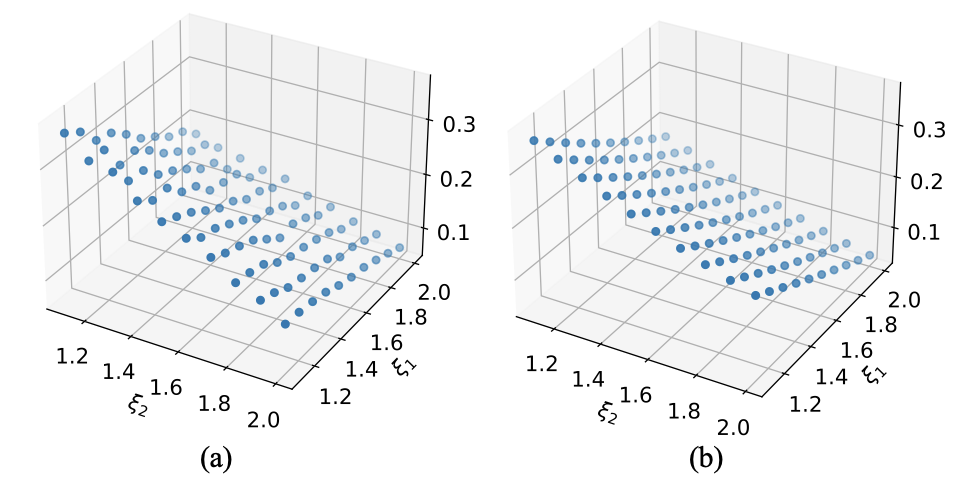
\includegraphics[width=0.45\textwidth]{Figures/value_func_visual.png}
%     \caption{Exponential of value function at $t=0$ (a) from solving the optimal control with Riccati equations, (b) from the PINN prediction.
%     }
%     \label{fig:value_function_3d->2d}
% \end{figure}

  % \begin{figure}[t]
  % \begin{subfigure}{0.45\columnwidth}
  % 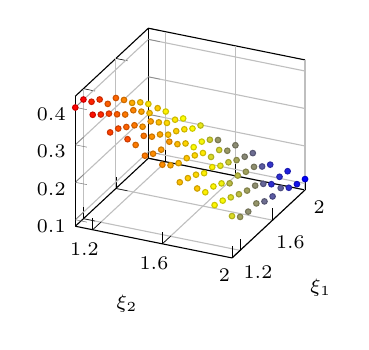
\begin{tikzpicture}
 
\begin{axis}[
% hide x axis,
% hide y axis,
% tick align=outside,
tick pos=left,
% x grid style={darkgray176},
% xlabel style={rotate=-10},
xlabel={\(\displaystyle \xi_2\)},
xtick = {1.2,1.6,2},
% xmin=1.0395, xmax=1.1605,
xtick style={color=black},
% y grid style={darkgray176},
% ylabel style={rotate=45},
ylabel={\(\displaystyle \xi_1\)},
ytick = {1.2,1.6,2},
% ymin=1.0395, ymax=1.1605,
ytick style={color=black},
% yticklabel style={anchor=center}
ztick = {0.1,0.2,0.3,0.4},
width=4.5cm,height=4.5cm,
font = \scriptsize, 
grid
]
 
\addplot3[
  mark=*,
  mark size=1pt,
  only marks,
  scatter,
  scatter/@post marker code/.code={%
  \endscope
},
%   scatter/@pre marker code/.code={%
%   \expanded{%
%   \noexpand\definecolor{thispointdrawcolor}{RGB}{\drawcolor}%
%   \noexpand\definecolor{thispointfillcolor}{RGB}{\fillcolor}%
%   }%
%   \scope[draw=thispointdrawcolor, fill=thispointfillcolor]%
% },
%   visualization depends on={value \thisrow{draw} \as \drawcolor},
%   visualization depends on={value \thisrow{fill} \as \fillcolor}
] table 
{
% x y   z
% 1.1 1.1   0.39946797
% 1.1 1.2 0.40073798
% }
x    y         z
 1.1  1.1  0.399468
 1.1  1.2  0.400738
 1.1  1.3   0.37457
 1.1  1.4  0.360488
 1.1  1.5  0.328584
 1.1  1.6  0.324079
 1.1  1.7  0.298825
 1.1  1.8   0.27083
 1.1  1.9    0.2521
 1.1  2.0  0.227553
 1.2  1.1  0.389525
 1.2  1.2  0.370092
 1.2  1.3  0.352291
 1.2  1.4  0.330356
 1.2  1.5  0.309561
 1.2  1.6  0.300812
 1.2  1.7  0.276975
 1.2  1.8  0.252998
 1.2  1.9  0.245923
 1.2  2.0  0.216798
 1.3  1.1  0.351917
 1.3  1.2   0.34194
 1.3  1.3  0.325988
 1.3  1.4  0.310379
 1.3  1.5  0.286387
 1.3  1.6  0.280482
 1.3  1.7   0.25777
 1.3  1.8  0.236114
 1.3  1.9  0.224505
 1.3  2.0  0.207655
 1.4  1.1   0.34314
 1.4  1.2  0.307621
 1.4  1.3  0.311731
 1.4  1.4   0.28943
 1.4  1.5  0.275154
 1.4  1.6  0.254513
 1.4  1.7  0.243731
 1.4  1.8  0.228482
 1.4  1.9  0.210313
 1.4  2.0  0.198334
 1.5  1.1  0.308505
 1.5  1.2   0.29355
 1.5  1.3   0.28427
 1.5  1.4    0.2854
 1.5  1.5  0.258761
 1.5  1.6  0.240411
 1.5  1.7  0.210336
 1.5  1.8  0.204956
 1.5  1.9  0.189817
 1.5  2.0   0.16893
 1.6  1.1  0.293874
 1.6  1.2  0.272323
 1.6  1.3  0.257784
 1.6  1.4  0.250918
 1.6  1.5  0.238079
 1.6  1.6  0.224349
 1.6  1.7   0.19364
 1.6  1.8  0.191998
 1.6  1.9  0.169856
 1.6  2.0  0.164362
 1.7  1.1  0.256447
 1.7  1.2  0.247281
 1.7  1.3  0.236253
 1.7  1.4  0.220246
 1.7  1.5  0.216236
 1.7  1.6   0.19967
 1.7  1.7  0.188838
 1.7  1.8  0.174403
 1.7  1.9  0.163284
 1.7  2.0  0.152871
 1.8  1.1  0.249276
 1.8  1.2  0.218992
 1.8  1.3   0.21435
 1.8  1.4  0.202368
 1.8  1.5  0.182429
 1.8  1.6  0.182966
 1.8  1.7  0.172841
 1.8  1.8  0.165818
 1.8  1.9  0.146673
 1.8  2.0   0.13143
 1.9  1.1  0.214343
 1.9  1.2   0.20608
 1.9  1.3  0.194687
 1.9  1.4  0.182887
 1.9  1.5  0.172344
 1.9  1.6  0.165432
 1.9  1.7  0.150118
 1.9  1.8  0.128952
 1.9  1.9  0.128543
 1.9  2.0  0.123256
 2.0  1.1  0.194454
 2.0  1.2  0.171992
 2.0  1.3  0.165933
 2.0  1.4  0.167728
 2.0  1.5  0.152967
 2.0  1.6  0.146089
 2.0  1.7  0.148348
 2.0  1.8  0.128912
 2.0  1.9  0.118328
 2.0  2.0  0.111661
};
\end{axis}
 
\end{tikzpicture}


  % \caption{}
  % \end{subfigure}
  % % \hfill
  % \hspace{3pt}
  % \begin{subfigure}{0.45\columnwidth}
  % 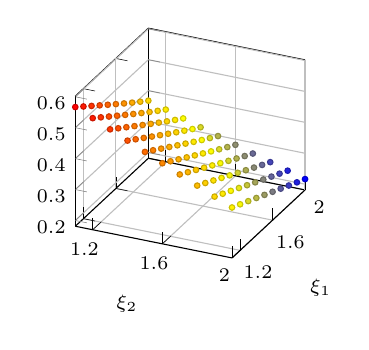
\begin{tikzpicture}
 
\begin{axis}[
% hide x axis,
% hide y axis,
% tick align=outside,
tick pos=left,
% x grid style={darkgray176},
% xlabel style={rotate=-10},
grid,
xlabel={\(\displaystyle \xi_2\)},
% xmin=1.0395, xmax=1.1605,
xtick style={color=black},
xtick = {1.2,1.6,2},
% y grid style={darkgray176},
% ylabel style={rotate=45},
ylabel={\(\displaystyle \xi_1\)},
% ymin=1.0395, ymax=1.1605,
ytick style={color=black},
ytick = {1.2,1.6,2},
% yticklabel style={anchor=center}
ztick = {0,0.1,0.2,0.3,0.4,0.5,0.6},
width=4.5cm,height=4.5cm,
font = \scriptsize, 
]
 
\addplot3[
  mark=*,
  mark size=1pt,
  only marks,
  scatter,
  scatter/@post marker code/.code={%
  \endscope
},
%   scatter/@pre marker code/.code={%
%   \expanded{%
%   \noexpand\definecolor{thispointdrawcolor}{RGB}{\drawcolor}%
%   \noexpand\definecolor{thispointfillcolor}{RGB}{\fillcolor}%
%   }%
%   \scope[draw=thispointdrawcolor, fill=thispointfillcolor]%
% },
%   visualization depends on={value \thisrow{draw} \as \drawcolor},
%   visualization depends on={value \thisrow{fill} \as \fillcolor}
] table 
{
% x y   z
% 1.1 1.1   0.39946797
% 1.1 1.2 0.40073798
% }
x    y         z
1.1  1.1  0.566776
 1.1  1.2    0.5442
 1.1  1.3  0.521572
 1.1  1.4  0.498963
 1.1  1.5  0.476445
 1.1  1.6  0.454088
 1.1  1.7  0.431963
 1.1  1.8  0.410133
 1.1  1.9  0.388662
 1.1  2.0  0.367607
 1.2  1.1  0.542305
 1.2  1.2  0.520507
 1.2  1.3  0.498673
 1.2  1.4  0.476866
 1.2  1.5  0.455153
 1.2  1.6  0.433599
 1.2  1.7  0.412271
 1.2  1.8   0.39123
 1.2  1.9  0.370534
 1.2  2.0  0.350237
 1.3  1.1  0.517474
 1.3  1.2  0.496528
 1.3  1.3  0.475552
 1.3  1.4  0.454605
 1.3  1.5  0.433748
 1.3  1.6  0.413043
 1.3  1.7  0.392553
 1.3  1.8  0.372335
 1.3  1.9  0.352445
 1.3  2.0  0.332934
 1.4  1.1   0.49241
 1.4  1.2  0.472376
 1.4  1.3  0.452311
 1.4  1.4   0.43227
 1.4  1.5  0.412308
 1.4  1.6  0.392486
 1.4  1.7  0.372862
 1.4  1.8  0.353492
 1.4  1.9   0.33443
 1.4  2.0  0.315723
 1.5  1.1  0.467252
 1.5  1.2  0.448174
 1.5  1.3  0.429059
 1.5  1.4  0.409956
 1.5  1.5  0.390918
 1.5  1.6  0.372001
 1.5  1.7  0.353262
 1.5  1.8  0.334755
 1.5  1.9  0.316531
 1.5  2.0  0.298637
 1.6  1.1  0.442137
 1.6  1.2  0.424046
 1.6  1.3  0.405906
 1.6  1.4  0.387762
 1.6  1.5  0.369663
 1.6  1.6  0.351664
 1.6  1.7  0.333818
 1.6  1.8  0.316179
 1.6  1.9  0.298796
 1.6  2.0  0.281715
 1.7  1.1  0.417195
 1.7  1.2  0.400108
 1.7  1.3  0.382958
 1.7  1.4  0.365782
 1.7  1.5  0.348628
 1.7  1.6  0.331548
 1.7  1.7  0.314595
 1.7  1.8  0.297821
 1.7  1.9  0.281273
 1.7  2.0  0.264998
 1.8  1.1  0.392542
 1.8  1.2  0.376467
 1.8  1.3  0.360309
 1.8  1.4  0.344101
 1.8  1.5   0.32789
 1.8  1.6  0.311724
 1.8  1.7  0.295655
 1.8  1.8  0.279734
 1.8  1.9  0.264009
 1.8  2.0  0.248526
 1.9  1.1  0.368282
 1.9  1.2  0.353214
 1.9  1.3  0.338041
 1.9  1.4  0.322794
 1.9  1.5  0.307514
 1.9  1.6   0.29225
 1.9  1.7   0.27705
 1.9  1.8  0.261966
 1.9  1.9  0.247046
 1.9  2.0  0.232335
 2.0  1.1  0.344499
 2.0  1.2  0.330425
 2.0  1.3  0.316224
 2.0  1.4  0.301921
 2.0  1.5  0.287557
 2.0  1.6  0.273176
 2.0  1.7  0.258826
 2.0  1.8  0.244558
 2.0  1.9  0.230421
 2.0  2.0   0.21646
};
\end{axis}
 
\end{tikzpicture}


  % \caption{} 
  % \end{subfigure} 
  % \caption{Exponential of value function at $t=0.5$ (a) from solving the optimal control with Riccati equations, (b) from the PINN prediction.}
  % \label{fig:value_func_visual}
  % \end{figure}


\begin{figure}[t]
    % \hspace{0pt}
  \begin{subfigure}{0.49\columnwidth}
  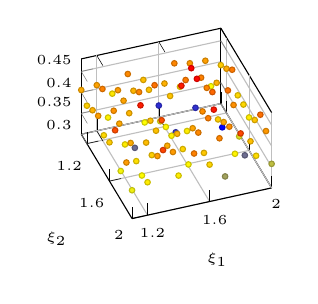
\begin{tikzpicture}
 
\begin{axis}[
% hide x axis,
% hide y axis,
% tick align=outside,
view/h=70,
view/v=50,
tick pos=left,
% x grid style={darkgray176},
% xlabel style={rotate=-10},
xlabel={\(\displaystyle \xi_2\)},
xtick = {1.2,1.6,2},
% xmin=1.0395, xmax=1.1605,
xtick style={color=black},
% y grid style={darkgray176},
% ylabel style={rotate=45},
ylabel={\(\displaystyle \xi_1\)},
ytick = {1.2,1.6,2},
% ymin=1.0395, ymax=1.1605,
ytick style={color=black},
% yticklabel style={anchor=center}
ztick = {0.3, 0.35, 0.4, 0.45},
zmin = 0.3, zmax = 0.48,
width=4cm,height=4cm,
font = \tiny, 
grid
]
 
\addplot3[
  mark=*,
  mark size=1pt,
  only marks,
  scatter,
  scatter/@post marker code/.code={%
  \endscope
},
%   scatter/@pre marker code/.code={%
%   \expanded{%
%   \noexpand\definecolor{thispointdrawcolor}{RGB}{\drawcolor}%
%   \noexpand\definecolor{thispointfillcolor}{RGB}{\fillcolor}%
%   }%
%   \scope[draw=thispointdrawcolor, fill=thispointfillcolor]%
% },
%   visualization depends on={value \thisrow{draw} \as \drawcolor},
%   visualization depends on={value \thisrow{fill} \as \fillcolor}
] table 
{
% x y   z
% 1.1 1.1   0.39946797
% 1.1 1.2 0.40073798
% }
x    y         z
1.1	1.1	0.40565765
1.1	1.2	0.40906673
1.1	1.3	0.38070724
1.1	1.4	0.41947888
1.1	1.5	0.39722215
1.1	1.6	0.327815  
1.1	1.7	0.42057389
1.1	1.8	0.4125304 
1.1	1.9	0.41043739
1.1	2.0	0.39177632
1.2	1.1	0.39057698
1.2	1.2	0.42240288
1.2	1.3	0.41134408
1.2	1.4	0.40181783
1.2	1.5	0.39592508
1.2	1.6	0.4028499 
1.2	1.7	0.38691981
1.2	1.8	0.32852271
1.2	1.9	0.37189909
1.2	2.0	0.40569639
1.3	1.1	0.4021314 
1.3	1.2	0.37647653
1.3	1.3	0.40863601
1.3	1.4	0.42108011
1.3	1.5	0.42933735
1.3	1.6	0.39541396
1.3	1.7	0.42539899
1.3	1.8	0.42294425
1.3	1.9	0.40247396
1.3	2.0	0.42562671
1.4	1.1	0.41106665
1.4	1.2	0.41515223
1.4	1.3	0.40118414
1.4	1.4	0.37091946
1.4	1.5	0.36558178
1.4	1.6	0.33109136
1.4	1.7	0.47613098
1.4	1.8	0.42098295
1.4	1.9	0.31857162
1.4	2.0	0.38683164
1.5	1.1	0.38704072
1.5	1.2	0.40674994
1.5	1.3	0.34074324
1.5	1.4	0.39740023
1.5	1.5	0.37438479
1.5	1.6	0.46459003
1.5	1.7	0.47303517
1.5	1.8	0.43332828
1.5	1.9	0.42910044
1.5	2.0	0.38717436
1.6	1.1	0.39256698
1.6	1.2	0.37941244
1.6	1.3	0.46470152
1.6	1.4	0.39593074
1.6	1.5	0.37578946
1.6	1.6	0.37891176
1.6	1.7	0.4175584 
1.6	1.8	0.3902694 
1.6	1.9	0.41664273
1.6	2.0	0.37877905
1.7	1.1	0.44378004
1.7	1.2	0.40528874
1.7	1.3	0.3980817 
1.7	1.4	0.44333453
1.7	1.5	0.40275016
1.7	1.6	0.40793259
1.7	1.7	0.42380686
1.7	1.8	0.4063768 
1.7	1.9	0.36389793
1.7	2.0	0.39502977
1.8	1.1	0.36884713
1.8	1.2	0.38433559
1.8	1.3	0.39053864
1.8	1.4	0.40482896
1.8	1.5	0.38869122
1.8	1.6	0.41995875
1.8	1.7	0.4666564 
1.8	1.8	0.41770006
1.8	1.9	0.34124801
1.8	2.0	0.43008697
1.9	1.1	0.41154597
1.9	1.2	0.37233469
1.9	1.3	0.41076619
1.9	1.4	0.41227455
1.9	1.5	0.37438566
1.9	1.6	0.3938453 
1.9	1.7	0.42059355
1.9	1.8	0.37538536
1.9	1.9	0.39709385
1.9	2.0	0.41333092
2.0	1.1	0.36769539
2.0	1.2	0.37862954
2.0	1.3	0.44736103
2.0	1.4	0.37825467
2.0	1.5	0.4228928 
2.0	1.6	0.38815098
2.0	1.7	0.35185788
2.0	1.8	0.44647427
2.0	1.9	0.38486582
2.0	2.0	0.3575396 
};
\end{axis}
 
\end{tikzpicture}


  \phantomsubcaption
  % \caption{}
  \end{subfigure}
  % \hfill
  % \hspace{0pt}
  \begin{subfigure}{0.49\columnwidth}
  % \def\axisdefaultticklabel{$\pgfmathprintnumber{\tick}$}

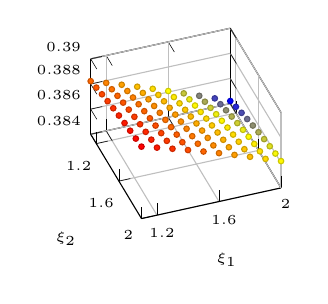
\begin{tikzpicture}
 
\begin{axis}[
% hide x axis,
% hide y axis,
% tick align=outside,
view/h=70,
view/v=50,
tick pos=left,
% x grid style={darkgray176},
% xlabel style={rotate=-10},
xlabel={\(\displaystyle \xi_2\)},
xtick = {1.2,1.6,2},
% xmin=1.0395, xmax=1.1605,
xtick style={color=black},
% y grid style={darkgray176},
% ylabel style={rotate=45},
ylabel={\(\displaystyle \xi_1\)},
ytick = {1.2,1.6,2},
% ymin=1.0395, ymax=1.1605,
ytick style={color=black},
% yticklabel style={anchor=center}
% zticklabels = {0.387,0.389,0.39, 0.392},
z tick label style={/pgf/number format/precision=3},
zmin=0.384, zmax=0.39,
ztick style={color=black},
width=4cm,height=4cm,
font = \tiny, 
grid
]
 
\addplot3[
  mark=*,
  mark size=1pt,
  only marks,
  scatter,
  scatter/@post marker code/.code={%
  \endscope
},
%   scatter/@pre marker code/.code={%
%   \expanded{%
%   \noexpand\definecolor{thispointdrawcolor}{RGB}{\drawcolor}%
%   \noexpand\definecolor{thispointfillcolor}{RGB}{\fillcolor}%
%   }%
%   \scope[draw=thispointdrawcolor, fill=thispointfillcolor]%
% },
%   visualization depends on={value \thisrow{draw} \as \drawcolor},
%   visualization depends on={value \thisrow{fill} \as \fillcolor}
] table 
{
% x y   z
% 1.1 1.1   0.39946797
% 1.1 1.2 0.40073798
% }
x    y         z
1.1	1.1	0.38822708
1.1	1.2	0.3878177 
1.1	1.3	0.3873986 
1.1	1.4	0.38696966
1.1	1.5	0.38653117
1.1	1.6	0.38608363
1.1	1.7	0.38562652
1.1	1.8	0.38516018
1.1	1.9	0.38468498
1.1	2.0	0.384201  
1.2	1.1	0.38845968
1.2	1.2	0.38805744
1.2	1.3	0.38764504
1.2	1.4	0.3872227 
1.2	1.5	0.38679066
1.2	1.6	0.38634878
1.2	1.7	0.38589743
1.2	1.8	0.3854364 
1.2	1.9	0.3849663 
1.2	2.0	0.38448724
1.3	1.1	0.3886749 
1.3	1.2	0.38827953
1.3	1.3	0.3878741 
1.3	1.4	0.3874583 
1.3	1.5	0.38703215
1.3	1.6	0.38659596
1.3	1.7	0.38615018
1.3	1.8	0.38569444
1.3	1.9	0.38522935
1.3	2.0	0.3847548 
1.4	1.1	0.3888729 
1.4	1.2	0.3884847 
1.4	1.3	0.38808578
1.4	1.4	0.38767618
1.4	1.5	0.38725623
1.4	1.6	0.3868259 
1.4	1.7	0.38638523
1.4	1.8	0.3859346 
1.4	1.9	0.38547435
1.4	2.0	0.38500416
1.5	1.1	0.38905445
1.5	1.2	0.38867337
1.5	1.3	0.3882807 
1.5	1.4	0.38787726
1.5	1.5	0.3874631 
1.5	1.6	0.3870382 
1.5	1.7	0.38660288
1.5	1.8	0.3861572 
1.5	1.9	0.38570136
1.5	2.0	0.3852356 
1.6	1.1	0.3892199 
1.6	1.2	0.38884515
1.6	1.3	0.3884591 
1.6	1.4	0.38806176
1.6	1.5	0.38765323
1.6	1.6	0.38723376
1.6	1.7	0.38680342
1.6	1.8	0.38636228
1.6	1.9	0.38591096
1.6	2.0	0.3854493 
1.7	1.1	0.38936958
1.7	1.2	0.38900158
1.7	1.3	0.38862154
1.7	1.4	0.38823003
1.7	1.5	0.387827  
1.7	1.6	0.38741255
1.7	1.7	0.38698718
1.7	1.8	0.3865506 
1.7	1.9	0.38610354
1.7	2.0	0.38564584
1.8	1.1	0.38950405
1.8	1.2	0.3891423 
1.8	1.3	0.38876835
1.8	1.4	0.3883825 
1.8	1.5	0.3879847 
1.8	1.6	0.38757548
1.8	1.7	0.3871547 
1.8	1.8	0.38672248
1.8	1.9	0.38627943
1.8	2.0	0.3858254 
1.9	1.1	0.38962328
1.9	1.2	0.38926792
1.9	1.3	0.3888999 
1.9	1.4	0.38851953
1.9	1.5	0.38812703
1.9	1.6	0.38772246
1.9	1.7	0.38730612
1.9	1.8	0.38687834
1.9	1.9	0.38643894
1.9	2.0	0.3859885 
2.0	1.1	0.38972837
2.0	1.2	0.38937902
2.0	1.3	0.38901663
2.0	1.4	0.3886415 
2.0	1.5	0.38825408
2.0	1.6	0.38785404
2.0	1.7	0.38744193
2.0	1.8	0.38701817
2.0	1.9	0.3865824 
2.0	2.0	0.38613522
};
\end{axis}
 
\end{tikzpicture}


  \phantomsubcaption
  % \caption{} 
  \end{subfigure} 
  \vspace{-0.3em}
  \caption{Estimation of the exponential of value function at $t=0.5$ for a 1000-dimensional system by path integral MC (left), and by the proposed method (right).}
   % \vspace{-1.6em}
  \label{fig:value_func_visual_1000d}
\end{figure}
  
% \subsection{Safety Probability Estimation}
% \todo{consider moving this part to appendix to save space}
% We consider the same 3-dimensional system~\eqref{eq:3d_system_experiment} and set the nominal controller to be $\mathcal{N}(x) \equiv 0$. We consider safe set~\eqref{eq:safe set definition} with barrier function $\phi(x) = \min\{-(x_1+x_2), -x_3\}+5$. We pick the same features as~\eqref{eq:3d_features} and we have $\alpha_i$ and $\beta_i$ as in~\eqref{eq:1000d_alpha_beta} for $i = 1,2$. Then the barrier function can be written as
% \begin{equation}
%     r(\xi) = \min\{-\xi_1, -\xi_2\}+5,
% \end{equation}
% and the set $\mathcal{B} = \{\xi: r(\xi) \geq 0\} = (-\infty,5] \times (-\infty,5]$. The PDE that governs the evolution of the safety probability is given by
% \begin{equation}
% \begin{aligned}
%     & 0 = \frac{\partial \mu}{\partial t} - 
%     \alpha(\xi) \beta(\xi) \frac{\partial \mu}{\partial \xi} - \frac{1}{2} \operatorname{Tr} \left(\mathbf{a}(\xi) \frac{\partial^2 \mu}{\partial \xi^2} \right)  \\
%     & = \frac{\partial \mu}{\partial t} - \xi_1 \frac{\partial \mu}{\partial \xi_1} - \xi_2 \frac{\partial \mu}{\partial \xi_2} - \frac{\partial^2 \mu}{\partial \xi_1^2} - \frac{1}{2} \frac{\partial^2 \mu}{\partial \xi_2^2} 
% \end{aligned}
% \end{equation}
% \begin{equation}
%     \mu(\xi,0)  =1, \,\, \xi \in \mathcal{B}; \quad \mu(\xi,t) =0, \,\, \xi \in \partial \mathcal{B}.
% \end{equation}
% We use the same procedure to train a PINN for $\bar F(x,t)$ on spatial-temporal space $\Omega \times \mathbb{T} = [1,4]^2 \times [0,1]$, with grid size $d\xi = 0.1$ and $dt = 0.1$. Fig.~\ref{fig:safe_prob_3d->2d} shows the estimated safety probability from MC simulation and the PINN prediction. 
% % Similarly, we observe accurate estimations of the safety probability from PINN with generalization to unseen region in the state space and to longer time horizons.
% We can see that the proposed method is able to estimate safety probability at unseen regions in the state space, generalize to longer time horizons, and does so with higher accuracy than the MC method.


% % \begin{figure}[t]
% %     \centering
% %     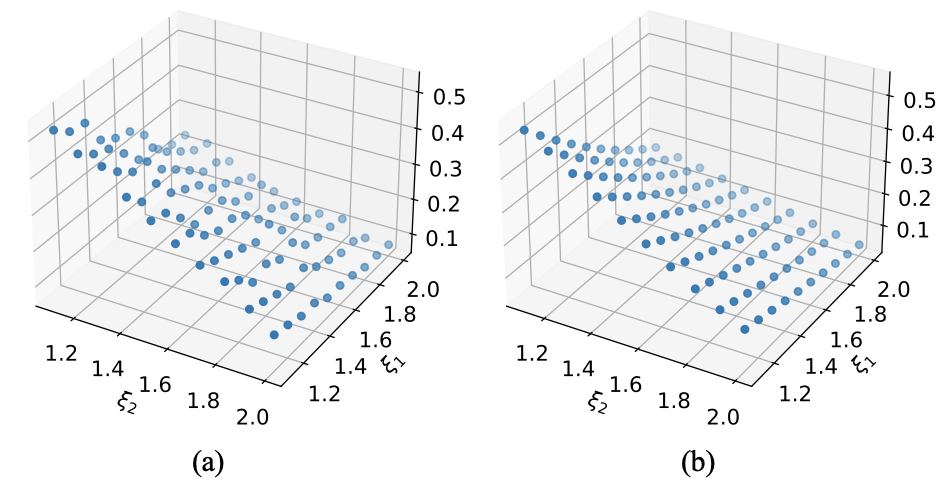
\includegraphics[width=0.45\textwidth]{Figures/safe_prob_visual.png}
% %     \caption{Safety probability at $t = 1$ (a) from MC simulation, (b) from the PINN prediction.
% %     }
% %     \label{fig:safe_prob_3d->2d}
% % \end{figure}

% \begin{figure}[t]
%   \begin{subfigure}{0.45\columnwidth}
%   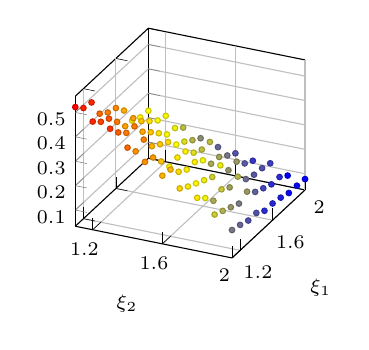
\begin{tikzpicture}
 
\begin{axis}[
% hide x axis,
% hide y axis,
% tick align=outside,
tick pos=left,
% x grid style={darkgray176},
% xlabel style={rotate=-10},
xlabel={\(\displaystyle \xi_2\)},
xtick = {1.2,1.6,2},
% xmin=1.0395, xmax=1.1605,
xtick style={color=black},
% y grid style={darkgray176},
% ylabel style={rotate=45},
ylabel={\(\displaystyle \xi_1\)},
ytick = {1.2,1.6,2},
% ymin=1.0395, ymax=1.1605,
ytick style={color=black},
% yticklabel style={anchor=center}
ztick = {0.1,0.2,0.3,0.4,0.5},
width=4.5cm,height=4.5cm,
font = \scriptsize, 
grid
]
 
\addplot3[
  mark=*,
  mark size=1pt,
  only marks,
  scatter,
  scatter/@post marker code/.code={%
  \endscope
},
%   scatter/@pre marker code/.code={%
%   \expanded{%
%   \noexpand\definecolor{thispointdrawcolor}{RGB}{\drawcolor}%
%   \noexpand\definecolor{thispointfillcolor}{RGB}{\fillcolor}%
%   }%
%   \scope[draw=thispointdrawcolor, fill=thispointfillcolor]%
% },
%   visualization depends on={value \thisrow{draw} \as \drawcolor},
%   visualization depends on={value \thisrow{fill} \as \fillcolor}
] table 
{
x    y         z
 1.1  1.1  0.522
 1.1  1.2  0.487
 1.1  1.3  0.479
 1.1  1.4  0.402
 1.1  1.5  0.376
 1.1  1.6  0.363
 1.1  1.7  0.322
 1.1  1.8   0.25
 1.1  1.9  0.232
 1.1  2.0  0.228
 1.2  1.1  0.477
 1.2  1.2  0.445
 1.2  1.3  0.427
 1.2  1.4  0.383
 1.2  1.5  0.334
 1.2  1.6  0.336
 1.2  1.7  0.293
 1.2  1.8  0.262
 1.2  1.9  0.234
 1.2  2.0  0.222
 1.3  1.1  0.462
 1.3  1.2  0.416
 1.3  1.3  0.383
 1.3  1.4  0.379
 1.3  1.5  0.326
 1.3  1.6  0.293
 1.3  1.7  0.258
 1.3  1.8  0.222
 1.3  1.9  0.217
 1.3  2.0  0.188
 1.4  1.1  0.399
 1.4  1.2  0.353
 1.4  1.3   0.37
 1.4  1.4  0.312
 1.4  1.5  0.289
 1.4  1.6  0.267
 1.4  1.7  0.226
 1.4  1.8  0.207
 1.4  1.9  0.182
 1.4  2.0  0.159
 1.5  1.1  0.355
 1.5  1.2  0.342
 1.5  1.3  0.295
 1.5  1.4  0.243
 1.5  1.5  0.249
 1.5  1.6  0.243
 1.5  1.7  0.207
 1.5  1.8  0.189
 1.5  1.9  0.189
 1.5  2.0  0.137
 1.6  1.1  0.313
 1.6  1.2  0.307
 1.6  1.3  0.267
 1.6  1.4  0.245
 1.6  1.5  0.245
 1.6  1.6  0.221
 1.6  1.7  0.176
 1.6  1.8  0.173
 1.6  1.9  0.148
 1.6  2.0  0.126
 1.7  1.1  0.275
 1.7  1.2  0.252
 1.7  1.3  0.234
 1.7  1.4  0.216
 1.7  1.5  0.198
 1.7  1.6  0.215
 1.7  1.7  0.164
 1.7  1.8  0.168
 1.7  1.9   0.13
 1.7  2.0   0.11
 1.8  1.1  0.251
 1.8  1.2  0.219
 1.8  1.3  0.177
 1.8  1.4  0.193
 1.8  1.5   0.17
 1.8  1.6  0.183
 1.8  1.7  0.142
 1.8  1.8  0.129
 1.8  1.9  0.125
 1.8  2.0  0.114
 1.9  1.1  0.197
 1.9  1.2  0.181
 1.9  1.3  0.165
 1.9  1.4  0.149
 1.9  1.5  0.167
 1.9  1.6  0.135
 1.9  1.7  0.119
 1.9  1.8  0.104
 1.9  1.9  0.103
 1.9  2.0  0.078
 2.0  1.1  0.148
 2.0  1.2  0.138
 2.0  1.3  0.125
 2.0  1.4  0.125
 2.0  1.5  0.103
 2.0  1.6  0.102
 2.0  1.7  0.095
 2.0  1.8  0.083
 2.0  1.9  0.082
 2.0  2.0  0.078
};
\end{axis}
 
\end{tikzpicture}


%   \caption{}
%   \end{subfigure}
%   % \hfill
%   \hspace{3pt}
%   \begin{subfigure}{0.45\columnwidth}
%   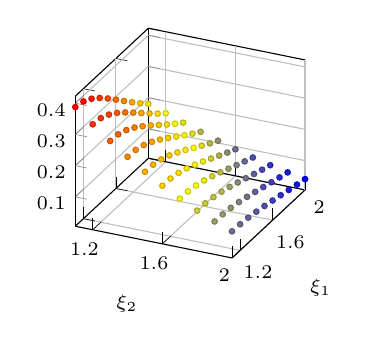
\begin{tikzpicture}
 
\begin{axis}[
% hide x axis,
% hide y axis,
% tick align=outside,
tick pos=left,
% x grid style={darkgray176},
% xlabel style={rotate=-10},
xlabel={\(\displaystyle \xi_2\)},
xtick = {1.2,1.6,2},
% xmin=1.0395, xmax=1.1605,
xtick style={color=black},
% y grid style={darkgray176},
% ylabel style={rotate=45},
ylabel={\(\displaystyle \xi_1\)},
ytick = {1.2,1.6,2},
% ymin=1.0395, ymax=1.1605,
ytick style={color=black},
% yticklabel style={anchor=center}
ztick = {0.1,0.2,0.3,0.4},
width=4.5cm,height=4.5cm,
font = \scriptsize, 
grid
]
 
\addplot3[
  mark=*,
  mark size=1pt,
  only marks,
  scatter,
  scatter/@post marker code/.code={%
  \endscope
},
%   scatter/@pre marker code/.code={%
%   \expanded{%
%   \noexpand\definecolor{thispointdrawcolor}{RGB}{\drawcolor}%
%   \noexpand\definecolor{thispointfillcolor}{RGB}{\fillcolor}%
%   }%
%   \scope[draw=thispointdrawcolor, fill=thispointfillcolor]%
% },
%   visualization depends on={value \thisrow{draw} \as \drawcolor},
%   visualization depends on={value \thisrow{fill} \as \fillcolor}
] table 
{
x    y         z
 1.1  1.1  0.387751
 1.1  1.2  0.381446
 1.1  1.3  0.366031
 1.1  1.4  0.344191
 1.1  1.5  0.318373
 1.1  1.6  0.290492
 1.1  1.7  0.261935
 1.1  1.8  0.233664
 1.1  1.9  0.206335
 1.1  2.0  0.180381
 1.2  1.1   0.34381
 1.2  1.2  0.339323
 1.2  1.3  0.326519
 1.2  1.4  0.307671
 1.2  1.5  0.284968
 1.2  1.6  0.260187
 1.2  1.7  0.234646
 1.2  1.8  0.209273
 1.2  1.9  0.184703
 1.2  2.0  0.161356
 1.3  1.1  0.301796
 1.3  1.2  0.298677
 1.3  1.3  0.288114
 1.3  1.4  0.271986
 1.3  1.5  0.252219
 1.3  1.6  0.230422
 1.3  1.7  0.207823
 1.3  1.8  0.185295
 1.3  1.9  0.163441
 1.3  2.0  0.142661
 1.4  1.1   0.26228
 1.4  1.2   0.26013
 1.4  1.3  0.251433
 1.4  1.4   0.23772
 1.4  1.5   0.22065
 1.4  1.6  0.201661
 1.4  1.7  0.181868
 1.4  1.8  0.162076
 1.4  1.9  0.142846
 1.4  2.0  0.124548
 1.5  1.1  0.225661
 1.5  1.2   0.22414
 1.5  1.3  0.216968
 1.5  1.4  0.205364
 1.5  1.5  0.190732
 1.5  1.6  0.174333
 1.5  1.7  0.157164
 1.5  1.8  0.139954
 1.5  1.9  0.123211
 1.5  2.0  0.107271
 1.6  1.1  0.192191
 1.6  1.2  0.191024
 1.6  1.3  0.185079
 1.6  1.4  0.175295
 1.6  1.5  0.162842
 1.6  1.6  0.148804
 1.6  1.7  0.134054
 1.6  1.8  0.119242
 1.6  1.9  0.104817
 1.6  2.0  0.091082
 1.7  1.1  0.162013
 1.7  1.2  0.160983
 1.7  1.3  0.156006
 1.7  1.4  0.147782
 1.7  1.5   0.13726
 1.7  1.6  0.125354
 1.7  1.7  0.112813
 1.7  1.8  0.100201
 1.7  1.9  0.087909
 1.7  2.0    0.0762
 1.8  1.1  0.135169
 1.8  1.2  0.134114
 1.8  1.3  0.129887
 1.8  1.4  0.122988
 1.8  1.5  0.114167
 1.8  1.6   0.10417
 1.8  1.7  0.093628
 1.8  1.8  0.083014
 1.8  1.9  0.072664
 1.8  2.0  0.062802
 1.9  1.1   0.11162
 1.9  1.2  0.110432
 1.9  1.3  0.106772
 1.9  1.4  0.100984
 1.9  1.5  0.093643
 1.9  1.6  0.085343
 1.9  1.7  0.076592
 1.9  1.8   0.06778
 1.9  1.9  0.059181
 1.9  2.0  0.050983
 2.0  1.1  0.091252
 2.0  1.2  0.089869
 2.0  1.3   0.08663
 2.0  1.4  0.081763
 2.0  1.5  0.075693
 2.0  1.6  0.068877
 2.0  1.7  0.061711
 2.0  1.8  0.054502
 2.0  1.9  0.047469
 2.0  2.0  0.040757
};
\end{axis}
 
\end{tikzpicture}


%   \caption{} 
%   \end{subfigure} 
%     \caption{Safety probability at $t = 1$ (a) from MC simulation, (b) from the PINN prediction.
%     }
%     \label{fig:safe_prob_3d->2d}
% \end{figure}

% \vspace{-0.5em}

\subsection{Sample Complexity}
We further examine the computation complexity of the proposed method to show its advantages in sample efficiency. We consider the problem of value function estimation of a 3-dimensional system with similar dynamics and cost defined in~\eqref{eq:1000d_system_experiment} and~\eqref{eq:1000d_system_experiment_cost}. 
% Due to space limit, please see extended version of the paper~\cite{} for details of the settings. \todo{} 
Please see appendix for details of the settings.
Fig.~\ref{fig:sample_complexity} shows the percentage error of the estimated value function with different number of samples for path integral MC and PINN with and without using comparison theorem for dimension reduction. The path integral MC with dimension reduction has sample complexities that are one order less than MC without dimension reduction, which indicates the efficacy of the dimension reduction scheme from the comparison theorem. The PINN further reduces sample complexity and achieves the best trade-off between accuracy and computation.
% \begin{figure}
%     \centering
%     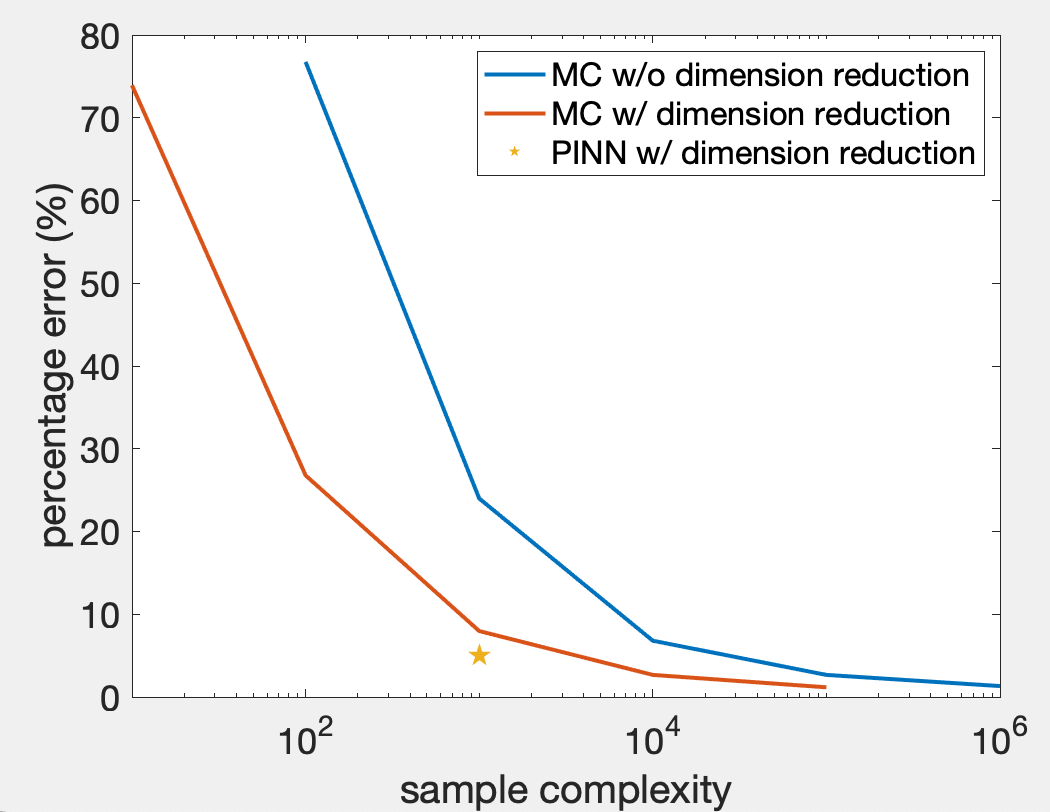
\includegraphics[width=0.36\textwidth]{Figures/sample_complexity.png}
%     \caption{Percentage error of the estimated value function with path integral MC.}
%     \todo{refine the plot, use pdf format}
%     \label{fig:sample_complexity}
% \end{figure}

\begin{figure}
    \centering
    % \pgfplotsset{width=7cm,height=3cm,compat=1.10}
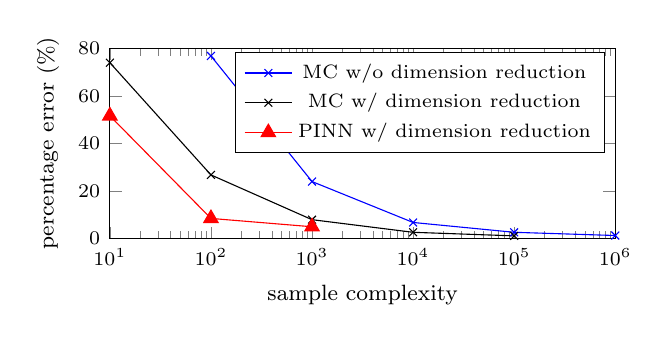
\begin{tikzpicture}
\begin{axis}[
    % x=0.5cm,
    % y=0.5cm/10,
    xlabel=\footnotesize{sample complexity},
    ylabel=\footnotesize{percentage error (\%)},
    xmode = log,
    xmin=10, xmax=10^6,
    ymin=0, ymax=80,
    % xtick={10^2,10^4,10^6},
    ytick={0,20,40,60,80},
    width=8cm,height=4cm,
    font = \scriptsize, 
            ]
\addplot[mark=x,blue] plot coordinates {
    (10^2,100*0.7675)
    (10^3,100*0.2399)
    (10^4,100*0.0680)
    (10^5,100*0.0267)
    (10^6,100*0.0132)    
};
\addlegendentry{MC w/o dimension reduction}

\addplot[color=black,mark=x,black]
    plot coordinates {
        (10^1,100*0.7392)
        (10^2,100*0.2678)
        (10^3,100*0.0797)
        (10^4,100*0.0267)
        (10^5,100*0.0117)
    };
\addlegendentry{MC w/ dimension reduction}

\addplot[color=red,mark=triangle*, mark size=3pt]
    plot coordinates {
        (10, 51.6)
        (100, 8.5)
        (1000,5)
    };
\addlegendentry{PINN w/ dimension reduction}
\end{axis}
\end{tikzpicture}
    \vspace{-0.5em}
    \caption{Percentage error of the estimated value function with path integral MC.}
    \vspace{-0.5em}
    \resolved{refine the plot, use pdf format}
    \label{fig:sample_complexity}
\end{figure}

\vspace{-0.3em}

\subsection{Feature Learning}
We verify our autoencoder-like network by learning the features and cost function in equations \eqref{eq:1000d_features} and~\eqref{eq: r_xi_1000d} for the 3-dimensional system described above. The network consists of 5 fully connected hidden layers of sizes 100, 10, 2, 10, 100, respectively, with the activation function as hyperbolic tangent. We use the Adam optimizer with initial learning rate set as 0.001. The parameters of the network are initialized via the Glorot uniform initialization. The weights in the loss function \eqref{eq: AE Loss} are set as $w_{RC}=1, \,w_{C.T.}=10$. The network is trained on a $[0, 1]^3$ state-space with grid size 0.01. The network successfully identified the features derived analytically in~\eqref{eq:3d_features} with $\mathrm{MSE}(\xi_1, \hat{\xi}_1)=0.2$ and $\mathrm{MSE}(\xi_2, \hat{\xi}_2)=0.06$. 
% See the following GitHub repository for value function estimation using learned features on more complex systems. 


\vspace{-0.3em}

\section{Conclusion}
\label{sec:conclusion}
% \todo{add}

We propose a unified framework for value function and safety probability estimation of high-dimensional stochastic systems. The novel dimensionality reduction technique uses the comparison theorem to generate low-dimensional stochastic processes that provide an exact characterization of the cost/barrier function, significantly improving sample complexity. We then transform the low-dimensional process into a low-dimensional PDE, and leverage physics-informed learning to generalize solutions into longer time horizons and unseen regions of state-space. We also achieve automatic feature identification through a specially designed autoencoder-like neural network. Experiment results show the efficacy of the proposed method. Future work includes application to multi-agent robotic control systems.

% \begin{figure}
%     \centering
%     %%%%%%%%%%
% by Xiyu
%%%%%%%%%%%

% color
\definecolor{color5}{HTML}{F2CC8F}
\definecolor{color2}{HTML}{F4F1DE}
\definecolor{color3}{HTML}{3D405B}
\definecolor{color4}{HTML}{81B29A}
\definecolor{color1}{HTML}{E07A5F}
\tikzset{
diagonal fill/.style 2 args={fill=#2, path picture={
\fill[#1, sharp corners] (path picture bounding box.south west) -|
                         (path picture bounding box.north east) -- cycle;}},
reversed diagonal fill/.style 2 args={fill=#2, path picture={
\fill[#1, sharp corners] (path picture bounding box.north west) |- 
                         (path picture bounding box.south east) -- cycle;}}
}

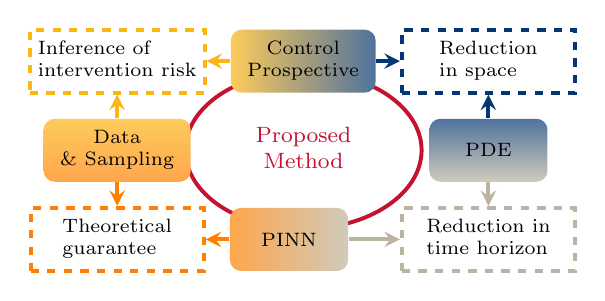
\begin{tikzpicture}[
    node distance = 4cm,
    node/.style={circle, fill=#1, inner sep=2pt, minimum size=0.7cm}, 
    edge/.style={-stealth, #1}
]

% 
\node[rectangle, draw=cmuyellow, dashed, line width=0.5mm, minimum height=0.8cm,minimum width=2.2cm,inner sep=-3pt] (t1){\scriptsize \begin{tabular}{ll}
% Observed data \\ to infer vs \\ the risk of\\ intervention.
Inference of \\ intervention risk
\end{tabular}};
\node[shading = axis, rectangle, left color= cmuyellow!70, right color= cmublue!70, minimum height=0.8cm,minimum width=1.5cm, rounded corners,inner sep=0pt] (control)[right=0.3cm of t1] {\scriptsize \begin{tabular}{cc}
Control \\ Prospective
\end{tabular}};

\node[rectangle, draw=cmublue, dashed, line width=0.5mm, minimum height=0.8cm,minimum width=2.2cm,inner sep=0pt] (t2) [right=0.3cm of control]{\scriptsize \begin{tabular}{ll}
Reduction \\ in space
\end{tabular}};

\node[shading = axis, rectangle, top color= cmuyellow!70, bottom color= orange!70, minimum height=0.8cm,minimum width=1.5cm, rounded corners, inner sep = 0pt] (sr) [below=0.3cm of t1] {\scriptsize \begin{tabular}{cc}
Data \\ \& Sampling\\
\end{tabular}};

\begin{scope}[on background layer]
\node[ellipse, draw = cmured, line width=0.5mm, minimum width = 3cm, minimum height = 2cm, rounded corners] (pm)[right= -0.1 cm of sr]{\footnotesize \textcolor{cmured}{\begin{tabular}{cc}
Proposed \\Method
\end{tabular}}};
\end{scope}

\node[shading = axis, rectangle, top color= cmublue!70, bottom color= cmutan!70, minimum height=0.8cm,minimum width=1.5cm, rounded corners] (pde) [below=0.3cm of t2] {\scriptsize PDE};

\node[rectangle, draw=orange, dashed, line width=0.5mm, minimum height=0.8cm,minimum width=2.2cm,inner sep=0pt] (t3)[below=0.3cm of sr]{\scriptsize \begin{tabular}{ll}
Theoretical \\ guarantee
\end{tabular}};

\node[shading = axis, rectangle, left color= orange!70, right color= cmutan!70,  minimum height=0.8cm,minimum width=1.5cm, rounded corners] (pinn)[right=0.3cm of t3]{\scriptsize PINN};

\node[rectangle, draw=cmutan, dashed, line width=0.5mm, minimum height=0.8cm,minimum width=2.2cm] (pw)[below=0.3cm of pde,inner sep=0pt]{\scriptsize \begin{tabular}{ll}
% Reduction in \\ time horizon \\due to PDE\\ constrains.
Reduction in \\ time horizon 
\end{tabular}};

%Edges
\draw[edge=cmuyellow,line width=0.5mm] (control) -> (t1);
\draw[edge=cmublue,line width=0.5mm] (control) -> (t2);
\draw[edge=cmuyellow,line width=0.5mm] (sr) -> (t1);
\draw[edge=cmublue,line width=0.5mm] (pde) -> (t2);
\draw[edge=orange,line width=0.5mm] (pinn) -> (t3);
\draw[edge=cmutan,line width=0.5mm] (pde) -> (pw);
\draw[edge=cmutan,line width=0.5mm] (pinn) -> (pw);
\draw[edge=orange,line width=0.5mm] (sr) -> (t3);
\end{tikzpicture}


% \begin{tikzpicture}[
%     node distance = 4cm,
%     node/.style={circle, fill=#1, inner sep=2pt, minimum size=0.7cm}, 
%     edge/.style={-stealth, #1}
% ]

% % 
% \node[rectangle, fill=newyellow,  line width=0.5mm, minimum height=0.8cm,minimum width=1.8cm,inner sep=-3pt] (t1){\scriptsize \begin{tabular}{ll}
% % Observed data \\ to infer vs \\ the risk of\\ intervention.
% Inference of \\ cost and risk
% \end{tabular}};

% \node[rectangle,  draw, line width = 0.3mm, minimum height=0.8cm,minimum width=1.8cm, inner sep=0pt] (control)[right=0.5cm of t1] {\scriptsize \begin{tabular}{cc}
% Control \\ Prospective
% \end{tabular}};

% % \node[rectangle,draw=cmuyellow,dash pattern= on 3pt off 5pt,line width = 0.3mm, minimum height=0.8cm,minimum width=1.8cm, inner sep=0pt,postaction={draw,cmublue,dash pattern= on 3pt off 5pt,dash phase=4pt,thick}] (control)[right=0.3cm of t1] {\scriptsize \begin{tabular}{cc}
% % Control \\ Prospective
% % \end{tabular}};


% \node[rectangle, fill=newblue,  line width=0.5mm, minimum height=0.8cm,minimum width=1.8cm,inner sep=0pt] (t2) [right=0.5cm of control]{\scriptsize \begin{tabular}{ll}
% Reduction \\ in space
% \end{tabular}};

% \node[draw, line width = 0.3mm, rectangle, minimum height=0.8cm,minimum width=1.8cm,  inner sep = 0pt] (sr) [below=0.3cm of t1] {\scriptsize \begin{tabular}{cc}
% Data \\ \& Sampling\\
% \end{tabular}};

% % \node[rectangle,draw=orange,dash pattern= on 3pt off 5pt,line width = 0.3mm, minimum height=0.8cm,minimum width=1.8cm, inner sep=0pt,postaction={draw,cmuyellow,dash pattern= on 3pt off 5pt,dash phase=4pt,thick}] (sr)[below=0.3cm of t1] {\scriptsize \begin{tabular}{cc}
% % Data \\ \& Sampling\\
% % \end{tabular}};

% % \begin{scope}[on background layer]
% % \node[rectangle, line width=0.5mm, minimum width = 3cm, minimum height = 2cm, rounded corners] (pm)[right= -0.1 cm of sr]{\scriptsize \begin{tabular}{cc}
% % Proposed \\Method
% % \end{tabular}};
% % \end{scope}

% \node[rectangle, minimum height=0.8cm,minimum width=1.8cm,  inner sep = 0pt] (pm) [below=0.3cm of control] {\footnotesize \begin{tabular}{cc}
% \underline{Proposed Method}
% % Proposed Method
% \end{tabular}};

% \node[rectangle, draw, line width = 0.3mm, minimum height=0.8cm,minimum width=1.8cm] (pde) [below=0.3cm of t2] {\scriptsize PDE};

% % \node[rectangle,draw=cmublue,dash pattern= on 3pt off 5pt,line width = 0.3mm, minimum height=0.8cm,minimum width=1.8cm, inner sep=0pt,postaction={draw,cmutan,dash pattern= on 3pt off 5pt,dash phase=4pt,thick}] (pde)[below=0.3cm of t2] {\scriptsize \begin{tabular}{cc}
% % PDE
% % \end{tabular}};

% \node[rectangle, fill=neworange,  line width=0.5mm, minimum height=0.8cm,minimum width=1.8cm,inner sep=0pt] (t3)[below=0.3cm of sr]{\scriptsize \begin{tabular}{ll}
% Theoretical \\ guarantee
% \end{tabular}};

% \node[rectangle, draw, line width = 0.3mm,  minimum height=0.8cm,minimum width=1.8cm] (pinn)[right=0.5cm of t3]{\scriptsize PINN};

% % \node[rectangle,draw=cmutan,dash pattern= on 3pt off 5pt,line width = 0.3mm, minimum height=0.8cm,minimum width=1.8cm, inner sep=0pt,postaction={draw,orange,dash pattern= on 3pt off 5pt,dash phase=4pt,thick}] (pinn)[right=0.3cm of t3] {\scriptsize \begin{tabular}{cc}
% % PINN
% % \end{tabular}};

% \node[rectangle, fill=newgray,  line width=0.5mm, minimum height=0.8cm,minimum width=1.8cm] (pw)[below=0.3cm of pde,inner sep=0pt]{\scriptsize \begin{tabular}{ll}
% % Reduction in \\ time horizon \\due to PDE\\ constrains.
% Reduction in \\ time horizon 
% \end{tabular}};

% %Edges
% \draw[edge=cmuyellow,line width=0.5mm] (control) -> (t1);
% \draw[edge=cmublue,line width=0.5mm] (control) -> (t2);
% \draw[edge=cmuyellow,line width=0.5mm] (sr) -> (t1);
% \draw[edge=cmublue,line width=0.5mm] (pde) -> (t2);
% \draw[edge=orange,line width=0.5mm] (pinn) -> (t3);
% \draw[edge=cmutan,line width=0.5mm] (pde) -> (pw);
% \draw[edge=cmutan,line width=0.5mm] (pinn) -> (pw);
% \draw[edge=orange,line width=0.5mm] (sr) -> (t3);
% \end{tikzpicture}
%     \caption{The overall diagram of the proposed method for stochastic optimal value function and safety probability estimation. \resolved{remove task x.x and replace with content in this paper}
%     }
%     \label{fig:overall_diagram}
% \end{figure}

% \clearpage


\bibliography{main}

\appendix


\section{Proof of Theorems}
In this section, we provide proof for Theorem~\ref{thm:comparison_lemma}, which is based on~\cite[Theorem 3.1]{ikeda1977comparison}.

\begin{proof}(Theorem~\ref{thm:comparison_lemma})
    Let $\xi_t$ be a stochastic process that characterizes the evolution of $p(x_t)$ with $x_t$ being sampled from system~\eqref{eq:continuous_dynamics} with $\xi_0 = p(x_0)$. From~\cite[Theorem 3.1]{ikeda1977comparison} we know the existence of such process $\xi_t$.
    Based on the definitions~\eqref{eq:a_b_def}, and according to~\cite[Theorem 3.1]{ikeda1977comparison}, we can construct the following four stochastic processes based on $a^\pm$ and $b^\pm$.
    \begin{equation}
    \label{eq:xi_process_++}
    \left\{\begin{aligned}
d \xi_t^{++} & =\sqrt{a^{+}\left(\xi_t^{++}\right)} d \widetilde{B}_t^{+}+a^{+}\left(\xi_t^{++}\right) b^{+}\left(\xi_t^{++}\right) d t, \\
\xi_0^{++} & =\xi_0 ,
\end{aligned}\right.
    \end{equation}
    \begin{equation}
    \label{eq:xi_process_+-}
        \left\{\begin{aligned}
d \xi_t^{+-} & =\sqrt{a^{+}\left(\xi_t^{+-}\right)} d \widetilde{B}_t^{+}+a^{+}\left(\xi_t^{+-}\right) b^{-}\left(\xi_t^{+-}\right) d t, \\
\xi_0^{+-} & =\xi_0,
\end{aligned}\right.
    \end{equation}
    \begin{equation}
    \label{eq:xi_process_-+}
        \left\{\begin{aligned}
d \xi_t^{-+} & =\sqrt{a^{-}\left(\xi_t^{-+}\right)} d \tilde{B}_t^{-}+a^{-}\left(\xi_t^{-+}\right) b^{-}\left(\xi_t^{-+}\right) d t, \\
\xi_t^{-+} & =\xi_0,
\end{aligned}\right.
    \end{equation}
    \begin{equation}
    \label{eq:xi_process_--}
        \left\{\begin{aligned}
d \xi_t^{--} & =\sqrt{a^{-}\left(\xi_t^{--}\right)} d \tilde{B}_t^{-}+a^{-}\left(\xi_t^{--}\right) b^{-}\left(\xi_t^{--}\right) d t, \\
\xi_0^{--} & =\xi_0,
\end{aligned}\right.
    \end{equation}
    where both $\widetilde{B}_t^{+}$ and $\widetilde{B}_t^{-}$ are one-dimensional Wiener processes, and we have $\xi_t^{--} \leq  \xi_t \leq \xi_t^{++}$ with probability 1.
    
    Given Assumption~\ref{asm:match_upper_lower_bound} holds, we know that $a^+(\xi) = a^-(\xi) = \alpha(\xi)$ and $b^+(\xi) = b^-(\xi) = \beta(\xi)$, $\forall \xi \in I$. Thus, the four stochastic processes~\eqref{eq:xi_process_++} - \eqref{eq:xi_process_--} are identical, which gives 
    \begin{equation}
        \xi_t^{++} = \xi_t^{+-} = \xi_t^{-+} = \xi_t^{--} = \xi_t.
    \end{equation}
    Replacing $\xi_t^{\pm \pm}$ with $\xi_t$, $a^\pm$ with $\alpha$ and $b^\pm$ with $\beta$, we have that $p(x_t)$ with $x_t$ being sampled from system~\eqref{eq:continuous_dynamics} is characterized by the following stochastic process
    \begin{equation}
% \label{eq:one_dim_xi_process}
    d \xi_t = \alpha\left(\xi_t\right) \beta\left(\xi_t\right) d t + \sqrt{\alpha\left(\xi_t\right)} d \tilde{B}_t,
\end{equation}
with $\xi_0 = p(x_0)$, and $\tilde{B}_t$ being a one-dimensional standard Wiener process.
    
    
    % $\bar \xi_t = \bar \xi_t^{\pm \pm}$ for all combinations of $\pm \pm$.
\end{proof}



\section{Details of the Sample Complexity Analysis}

In this section, we provide details of the sample complexity analysis. 

We consider a 3-dimensional system in which we want a 2-dimensional representation of the optimal value function. The system dynamics is given by
\begin{equation}
\label{eq:3d_system_experiment}
\begin{aligned}
    dx_1 &= (x_1 + x_3) \; dt + \sigma_1 (u_1 dt + dW_1) \\
    dx_2 &= (x_2 - x_3) \; dt + \sigma_2 (u_2 + dW_2) \\
    dx_3 &= x_3 \; dt + \sigma_3 (u_3 + dW_3)
\end{aligned}
\end{equation}
where $dW_i$ for $i = 1,2,3$ are standard Brownian motions and we assume $\sigma_i = 1$ for $i = 1,2,3$.
The running cost function is assumed to be
\begin{equation}
\label{eq:3d_system_experiment_cost}
    c(x) = \frac{1}{2}(x_1+x_2)^2 + \frac{1}{2}x_3^2.
\end{equation}
We pick two features of the state,
\begin{equation}
\label{eq:3d_features}
    \xi_1 = p_1(x) = x_1+x_2, \quad \xi_2 = p_2(x) = x_3.
\end{equation}
Then from~\eqref{eq:a_b_def}, we have
\begin{equation}
\label{eq:3d_alpha_beta}
\begin{aligned}
    \alpha_1(\xi_1) = 2, \,\, \alpha_2(\xi_2) = 1; \quad \beta_1(\xi_1) = \frac{\xi_1}{2}, \,\, \beta_2(\xi_2) = \xi_2
% \end{equation}
% \begin{equation}
    % \beta_1(\xi_1) = \frac{\xi_1}{2}, &
    % \frac{\begin{bmatrix}
    % 1 \\
    % 1 \\
    % 0
    % \end{bmatrix} \cdot \begin{bmatrix}
    % x_1 + x_3 \\
    % x_2 - x_3 \\
    % x_3
    % \end{bmatrix} }{a_1(x)} = \frac{x_1+x_2}{2} = \frac{\xi_1}{2},
    %\quad \beta_2(\xi_2) = \xi_2
   % % \frac{\begin{bmatrix}
    % 0 \\
    % 0 \\
    % 1
    % \end{bmatrix} \cdot \begin{bmatrix}
    % x_1 + x_3 \\
    % x_2 - x_3 \\
    % x_3
    % \end{bmatrix} }{a_2(x)} = x_3 = \xi_2
\end{aligned}
\end{equation}
thus satisfying Assumptions 2 and 3.
The cost function can then be written as
\begin{equation} \label{eq: r_xi}
    r(\xi) = \frac{1}{2}\xi_1^2 + \frac{1}{2}\xi_2^2.
\end{equation}
By the Feynman-Kac formula, we know that the exponential of the optimal value function $\varphi$ is the solution of the following PDE
\begin{align}
    & 0 = r(\xi)\mu 
    - \frac{\partial \mu}{\partial t} - 
    % \begin{bmatrix}
    % a_1 b_1 \\
    % a_2 b_2
    % \end{bmatrix} 
    \alpha(\xi) \beta(\xi) \frac{\partial \mu}{\partial \xi} - \frac{1}{2} \operatorname{Tr} \left(
    % \begin{bmatrix}
    % a_1 &  \\
    % & a_2 
    % \end{bmatrix} 
    \mathbf{a}(\xi) \frac{\partial^2 \mu}{\partial \xi^2} \right) \\
    & = (\frac{1}{2}\xi_1^2 + \frac{1}{2}\xi_2^2)\mu - \frac{\partial \mu}{\partial t} - \xi_1 \frac{\partial \mu}{\partial \xi_1} - \xi_2 \frac{\partial \mu}{\partial \xi_2} - \frac{\partial^2 \mu}{\partial \xi_1^2} - \frac{1}{2} \frac{\partial^2 \mu}{\partial \xi_2^2} \nonumber
\end{align}

\begin{equation}
    \mu(\xi, T) = \exp(- \frac{1}{2}\xi_1^2 - \frac{1}{2}\xi_2^2).
\end{equation}
With that, we generate data for $\bar \varphi(\xi,t)$ on feature-temporal space $\Omega \times \mathbb{T} = [1,2]^2 \times [0,1.5]$, with grid size $d\xi = 0.1$ and $dt = 0.1$ and train the PINN on $\Omega \times \mathbb{T} = [1,2]^2 \times [1,1.5]$. 
We use a PINN with 3 hidden layers and 32 neurons per layer to learn the value function $\hat \varphi$. The activation function is chosen as hyperbolic tangent function ($\tanh$). We use the Adam optimizer~\cite{kingma2014adam} for training with initial learning rate set as $0.001$. The PINN parameters $\boldsymbol\theta$ is initialized via Glorot uniform initialization and the weights in the loss function~\eqref{eq:PINN overall loss function} are set to be $\omega_p = \omega_d = 1$. Fig.~\ref{fig:value_func_visual} visualizes the estimated value function from the Riccati equation and the PINN prediction.

\begin{figure}[t]
  \begin{subfigure}{0.45\columnwidth}
  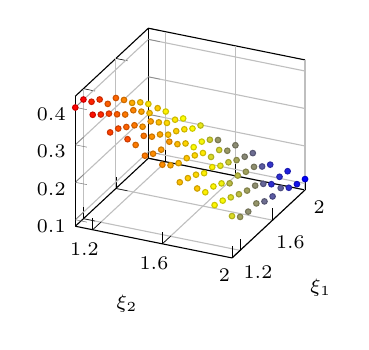
\begin{tikzpicture}
 
\begin{axis}[
% hide x axis,
% hide y axis,
% tick align=outside,
tick pos=left,
% x grid style={darkgray176},
% xlabel style={rotate=-10},
xlabel={\(\displaystyle \xi_2\)},
xtick = {1.2,1.6,2},
% xmin=1.0395, xmax=1.1605,
xtick style={color=black},
% y grid style={darkgray176},
% ylabel style={rotate=45},
ylabel={\(\displaystyle \xi_1\)},
ytick = {1.2,1.6,2},
% ymin=1.0395, ymax=1.1605,
ytick style={color=black},
% yticklabel style={anchor=center}
ztick = {0.1,0.2,0.3,0.4},
width=4.5cm,height=4.5cm,
font = \scriptsize, 
grid
]
 
\addplot3[
  mark=*,
  mark size=1pt,
  only marks,
  scatter,
  scatter/@post marker code/.code={%
  \endscope
},
%   scatter/@pre marker code/.code={%
%   \expanded{%
%   \noexpand\definecolor{thispointdrawcolor}{RGB}{\drawcolor}%
%   \noexpand\definecolor{thispointfillcolor}{RGB}{\fillcolor}%
%   }%
%   \scope[draw=thispointdrawcolor, fill=thispointfillcolor]%
% },
%   visualization depends on={value \thisrow{draw} \as \drawcolor},
%   visualization depends on={value \thisrow{fill} \as \fillcolor}
] table 
{
% x y   z
% 1.1 1.1   0.39946797
% 1.1 1.2 0.40073798
% }
x    y         z
 1.1  1.1  0.399468
 1.1  1.2  0.400738
 1.1  1.3   0.37457
 1.1  1.4  0.360488
 1.1  1.5  0.328584
 1.1  1.6  0.324079
 1.1  1.7  0.298825
 1.1  1.8   0.27083
 1.1  1.9    0.2521
 1.1  2.0  0.227553
 1.2  1.1  0.389525
 1.2  1.2  0.370092
 1.2  1.3  0.352291
 1.2  1.4  0.330356
 1.2  1.5  0.309561
 1.2  1.6  0.300812
 1.2  1.7  0.276975
 1.2  1.8  0.252998
 1.2  1.9  0.245923
 1.2  2.0  0.216798
 1.3  1.1  0.351917
 1.3  1.2   0.34194
 1.3  1.3  0.325988
 1.3  1.4  0.310379
 1.3  1.5  0.286387
 1.3  1.6  0.280482
 1.3  1.7   0.25777
 1.3  1.8  0.236114
 1.3  1.9  0.224505
 1.3  2.0  0.207655
 1.4  1.1   0.34314
 1.4  1.2  0.307621
 1.4  1.3  0.311731
 1.4  1.4   0.28943
 1.4  1.5  0.275154
 1.4  1.6  0.254513
 1.4  1.7  0.243731
 1.4  1.8  0.228482
 1.4  1.9  0.210313
 1.4  2.0  0.198334
 1.5  1.1  0.308505
 1.5  1.2   0.29355
 1.5  1.3   0.28427
 1.5  1.4    0.2854
 1.5  1.5  0.258761
 1.5  1.6  0.240411
 1.5  1.7  0.210336
 1.5  1.8  0.204956
 1.5  1.9  0.189817
 1.5  2.0   0.16893
 1.6  1.1  0.293874
 1.6  1.2  0.272323
 1.6  1.3  0.257784
 1.6  1.4  0.250918
 1.6  1.5  0.238079
 1.6  1.6  0.224349
 1.6  1.7   0.19364
 1.6  1.8  0.191998
 1.6  1.9  0.169856
 1.6  2.0  0.164362
 1.7  1.1  0.256447
 1.7  1.2  0.247281
 1.7  1.3  0.236253
 1.7  1.4  0.220246
 1.7  1.5  0.216236
 1.7  1.6   0.19967
 1.7  1.7  0.188838
 1.7  1.8  0.174403
 1.7  1.9  0.163284
 1.7  2.0  0.152871
 1.8  1.1  0.249276
 1.8  1.2  0.218992
 1.8  1.3   0.21435
 1.8  1.4  0.202368
 1.8  1.5  0.182429
 1.8  1.6  0.182966
 1.8  1.7  0.172841
 1.8  1.8  0.165818
 1.8  1.9  0.146673
 1.8  2.0   0.13143
 1.9  1.1  0.214343
 1.9  1.2   0.20608
 1.9  1.3  0.194687
 1.9  1.4  0.182887
 1.9  1.5  0.172344
 1.9  1.6  0.165432
 1.9  1.7  0.150118
 1.9  1.8  0.128952
 1.9  1.9  0.128543
 1.9  2.0  0.123256
 2.0  1.1  0.194454
 2.0  1.2  0.171992
 2.0  1.3  0.165933
 2.0  1.4  0.167728
 2.0  1.5  0.152967
 2.0  1.6  0.146089
 2.0  1.7  0.148348
 2.0  1.8  0.128912
 2.0  1.9  0.118328
 2.0  2.0  0.111661
};
\end{axis}
 
\end{tikzpicture}


  \caption{}
  \end{subfigure}
  % \hfill
  \hspace{3pt}
  \begin{subfigure}{0.45\columnwidth}
  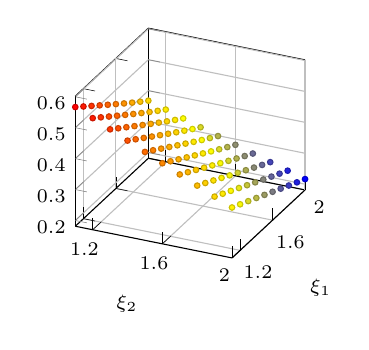
\begin{tikzpicture}
 
\begin{axis}[
% hide x axis,
% hide y axis,
% tick align=outside,
tick pos=left,
% x grid style={darkgray176},
% xlabel style={rotate=-10},
grid,
xlabel={\(\displaystyle \xi_2\)},
% xmin=1.0395, xmax=1.1605,
xtick style={color=black},
xtick = {1.2,1.6,2},
% y grid style={darkgray176},
% ylabel style={rotate=45},
ylabel={\(\displaystyle \xi_1\)},
% ymin=1.0395, ymax=1.1605,
ytick style={color=black},
ytick = {1.2,1.6,2},
% yticklabel style={anchor=center}
ztick = {0,0.1,0.2,0.3,0.4,0.5,0.6},
width=4.5cm,height=4.5cm,
font = \scriptsize, 
]
 
\addplot3[
  mark=*,
  mark size=1pt,
  only marks,
  scatter,
  scatter/@post marker code/.code={%
  \endscope
},
%   scatter/@pre marker code/.code={%
%   \expanded{%
%   \noexpand\definecolor{thispointdrawcolor}{RGB}{\drawcolor}%
%   \noexpand\definecolor{thispointfillcolor}{RGB}{\fillcolor}%
%   }%
%   \scope[draw=thispointdrawcolor, fill=thispointfillcolor]%
% },
%   visualization depends on={value \thisrow{draw} \as \drawcolor},
%   visualization depends on={value \thisrow{fill} \as \fillcolor}
] table 
{
% x y   z
% 1.1 1.1   0.39946797
% 1.1 1.2 0.40073798
% }
x    y         z
1.1  1.1  0.566776
 1.1  1.2    0.5442
 1.1  1.3  0.521572
 1.1  1.4  0.498963
 1.1  1.5  0.476445
 1.1  1.6  0.454088
 1.1  1.7  0.431963
 1.1  1.8  0.410133
 1.1  1.9  0.388662
 1.1  2.0  0.367607
 1.2  1.1  0.542305
 1.2  1.2  0.520507
 1.2  1.3  0.498673
 1.2  1.4  0.476866
 1.2  1.5  0.455153
 1.2  1.6  0.433599
 1.2  1.7  0.412271
 1.2  1.8   0.39123
 1.2  1.9  0.370534
 1.2  2.0  0.350237
 1.3  1.1  0.517474
 1.3  1.2  0.496528
 1.3  1.3  0.475552
 1.3  1.4  0.454605
 1.3  1.5  0.433748
 1.3  1.6  0.413043
 1.3  1.7  0.392553
 1.3  1.8  0.372335
 1.3  1.9  0.352445
 1.3  2.0  0.332934
 1.4  1.1   0.49241
 1.4  1.2  0.472376
 1.4  1.3  0.452311
 1.4  1.4   0.43227
 1.4  1.5  0.412308
 1.4  1.6  0.392486
 1.4  1.7  0.372862
 1.4  1.8  0.353492
 1.4  1.9   0.33443
 1.4  2.0  0.315723
 1.5  1.1  0.467252
 1.5  1.2  0.448174
 1.5  1.3  0.429059
 1.5  1.4  0.409956
 1.5  1.5  0.390918
 1.5  1.6  0.372001
 1.5  1.7  0.353262
 1.5  1.8  0.334755
 1.5  1.9  0.316531
 1.5  2.0  0.298637
 1.6  1.1  0.442137
 1.6  1.2  0.424046
 1.6  1.3  0.405906
 1.6  1.4  0.387762
 1.6  1.5  0.369663
 1.6  1.6  0.351664
 1.6  1.7  0.333818
 1.6  1.8  0.316179
 1.6  1.9  0.298796
 1.6  2.0  0.281715
 1.7  1.1  0.417195
 1.7  1.2  0.400108
 1.7  1.3  0.382958
 1.7  1.4  0.365782
 1.7  1.5  0.348628
 1.7  1.6  0.331548
 1.7  1.7  0.314595
 1.7  1.8  0.297821
 1.7  1.9  0.281273
 1.7  2.0  0.264998
 1.8  1.1  0.392542
 1.8  1.2  0.376467
 1.8  1.3  0.360309
 1.8  1.4  0.344101
 1.8  1.5   0.32789
 1.8  1.6  0.311724
 1.8  1.7  0.295655
 1.8  1.8  0.279734
 1.8  1.9  0.264009
 1.8  2.0  0.248526
 1.9  1.1  0.368282
 1.9  1.2  0.353214
 1.9  1.3  0.338041
 1.9  1.4  0.322794
 1.9  1.5  0.307514
 1.9  1.6   0.29225
 1.9  1.7   0.27705
 1.9  1.8  0.261966
 1.9  1.9  0.247046
 1.9  2.0  0.232335
 2.0  1.1  0.344499
 2.0  1.2  0.330425
 2.0  1.3  0.316224
 2.0  1.4  0.301921
 2.0  1.5  0.287557
 2.0  1.6  0.273176
 2.0  1.7  0.258826
 2.0  1.8  0.244558
 2.0  1.9  0.230421
 2.0  2.0   0.21646
};
\end{axis}
 
\end{tikzpicture}


  \caption{} 
  \end{subfigure} 
  \caption{Exponential of value function at $t=0.5$ (a) from solving the optimal control with Riccati equations, (b) from the PINN prediction.}
  \label{fig:value_func_visual}
\end{figure}

\section{Experiments for Safety Probability Estimation}

In this section, we present simulation results of the proposed method for safety probability estimation.

We consider the same 3-dimensional system~\eqref{eq:3d_system_experiment}
and we set the nominal controller to be $\mathcal{N}(x) \equiv 0$. We consider safe set~\eqref{eq:safe set definition} with barrier function $\phi(x) = \min\{-(x_1+x_2), -x_3\}+4$. We pick the same features as~\eqref{eq:3d_features} and we have $\alpha_i$ and $\beta_i$ as in~\eqref{eq:3d_alpha_beta} for $i = 1,2$. Then the barrier function can be written as
\begin{equation}
    r(\xi) = \min\{-\xi_1, -\xi_2\}+4,
\end{equation}
and the set $\mathcal{B} = \{\xi: r(\xi) \geq 0\} = (-\infty,4] \times (-\infty,4]$. The PDE that governs the evolution of the safety probability is given by
\begin{equation}
\begin{aligned}
    & 0 = \frac{\partial \mu}{\partial t} - 
    \alpha(\xi) \beta(\xi) \frac{\partial \mu}{\partial \xi} - \frac{1}{2} \operatorname{Tr} \left(\mathbf{a}(\xi) \frac{\partial^2 \mu}{\partial \xi^2} \right)  \\
    & = \frac{\partial \mu}{\partial t} - \xi_1 \frac{\partial \mu}{\partial \xi_1} - \xi_2 \frac{\partial \mu}{\partial \xi_2} - \frac{\partial^2 \mu}{\partial \xi_1^2} - \frac{1}{2} \frac{\partial^2 \mu}{\partial \xi_2^2} 
\end{aligned}
\end{equation}
\begin{equation}
    \mu(\xi,0)  =1, \,\, \xi \in \mathcal{B}; \quad \mu(\xi,t) =0, \,\, \xi \in \partial \mathcal{B}.
\end{equation}
We use the same procedure to train a PINN for $\bar F(\xi,t)$ on feature-temporal space $\Omega \times \mathbb{T} = [1,2]^2 \times [0,1]$, with grid size $d\xi = 0.1$ and $dt = 0.1$. Fig.~\ref{fig:safe_prob_3d->2d} shows the estimated safety probability from MC simulation and the PINN prediction. 
% Similarly, we observe accurate estimations of the safety probability from PINN with generalization to unseen region in the state space and to longer time horizons.
We can see that the proposed method is able to estimate safety probability at unseen regions in the state space, generalize to longer time horizons, and does so with higher accuracy than the MC method.

\begin{figure}[t]
  \begin{subfigure}{0.45\columnwidth}
  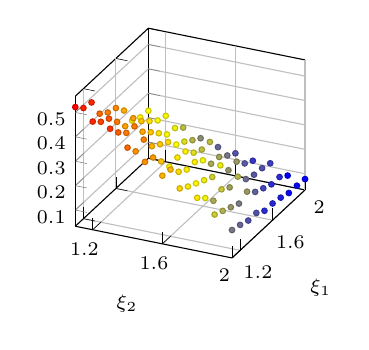
\begin{tikzpicture}
 
\begin{axis}[
% hide x axis,
% hide y axis,
% tick align=outside,
tick pos=left,
% x grid style={darkgray176},
% xlabel style={rotate=-10},
xlabel={\(\displaystyle \xi_2\)},
xtick = {1.2,1.6,2},
% xmin=1.0395, xmax=1.1605,
xtick style={color=black},
% y grid style={darkgray176},
% ylabel style={rotate=45},
ylabel={\(\displaystyle \xi_1\)},
ytick = {1.2,1.6,2},
% ymin=1.0395, ymax=1.1605,
ytick style={color=black},
% yticklabel style={anchor=center}
ztick = {0.1,0.2,0.3,0.4,0.5},
width=4.5cm,height=4.5cm,
font = \scriptsize, 
grid
]
 
\addplot3[
  mark=*,
  mark size=1pt,
  only marks,
  scatter,
  scatter/@post marker code/.code={%
  \endscope
},
%   scatter/@pre marker code/.code={%
%   \expanded{%
%   \noexpand\definecolor{thispointdrawcolor}{RGB}{\drawcolor}%
%   \noexpand\definecolor{thispointfillcolor}{RGB}{\fillcolor}%
%   }%
%   \scope[draw=thispointdrawcolor, fill=thispointfillcolor]%
% },
%   visualization depends on={value \thisrow{draw} \as \drawcolor},
%   visualization depends on={value \thisrow{fill} \as \fillcolor}
] table 
{
x    y         z
 1.1  1.1  0.522
 1.1  1.2  0.487
 1.1  1.3  0.479
 1.1  1.4  0.402
 1.1  1.5  0.376
 1.1  1.6  0.363
 1.1  1.7  0.322
 1.1  1.8   0.25
 1.1  1.9  0.232
 1.1  2.0  0.228
 1.2  1.1  0.477
 1.2  1.2  0.445
 1.2  1.3  0.427
 1.2  1.4  0.383
 1.2  1.5  0.334
 1.2  1.6  0.336
 1.2  1.7  0.293
 1.2  1.8  0.262
 1.2  1.9  0.234
 1.2  2.0  0.222
 1.3  1.1  0.462
 1.3  1.2  0.416
 1.3  1.3  0.383
 1.3  1.4  0.379
 1.3  1.5  0.326
 1.3  1.6  0.293
 1.3  1.7  0.258
 1.3  1.8  0.222
 1.3  1.9  0.217
 1.3  2.0  0.188
 1.4  1.1  0.399
 1.4  1.2  0.353
 1.4  1.3   0.37
 1.4  1.4  0.312
 1.4  1.5  0.289
 1.4  1.6  0.267
 1.4  1.7  0.226
 1.4  1.8  0.207
 1.4  1.9  0.182
 1.4  2.0  0.159
 1.5  1.1  0.355
 1.5  1.2  0.342
 1.5  1.3  0.295
 1.5  1.4  0.243
 1.5  1.5  0.249
 1.5  1.6  0.243
 1.5  1.7  0.207
 1.5  1.8  0.189
 1.5  1.9  0.189
 1.5  2.0  0.137
 1.6  1.1  0.313
 1.6  1.2  0.307
 1.6  1.3  0.267
 1.6  1.4  0.245
 1.6  1.5  0.245
 1.6  1.6  0.221
 1.6  1.7  0.176
 1.6  1.8  0.173
 1.6  1.9  0.148
 1.6  2.0  0.126
 1.7  1.1  0.275
 1.7  1.2  0.252
 1.7  1.3  0.234
 1.7  1.4  0.216
 1.7  1.5  0.198
 1.7  1.6  0.215
 1.7  1.7  0.164
 1.7  1.8  0.168
 1.7  1.9   0.13
 1.7  2.0   0.11
 1.8  1.1  0.251
 1.8  1.2  0.219
 1.8  1.3  0.177
 1.8  1.4  0.193
 1.8  1.5   0.17
 1.8  1.6  0.183
 1.8  1.7  0.142
 1.8  1.8  0.129
 1.8  1.9  0.125
 1.8  2.0  0.114
 1.9  1.1  0.197
 1.9  1.2  0.181
 1.9  1.3  0.165
 1.9  1.4  0.149
 1.9  1.5  0.167
 1.9  1.6  0.135
 1.9  1.7  0.119
 1.9  1.8  0.104
 1.9  1.9  0.103
 1.9  2.0  0.078
 2.0  1.1  0.148
 2.0  1.2  0.138
 2.0  1.3  0.125
 2.0  1.4  0.125
 2.0  1.5  0.103
 2.0  1.6  0.102
 2.0  1.7  0.095
 2.0  1.8  0.083
 2.0  1.9  0.082
 2.0  2.0  0.078
};
\end{axis}
 
\end{tikzpicture}


  \caption{}
  \end{subfigure}
  % \hfill
  \hspace{3pt}
  \begin{subfigure}{0.45\columnwidth}
  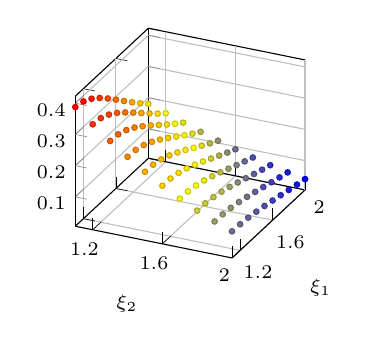
\begin{tikzpicture}
 
\begin{axis}[
% hide x axis,
% hide y axis,
% tick align=outside,
tick pos=left,
% x grid style={darkgray176},
% xlabel style={rotate=-10},
xlabel={\(\displaystyle \xi_2\)},
xtick = {1.2,1.6,2},
% xmin=1.0395, xmax=1.1605,
xtick style={color=black},
% y grid style={darkgray176},
% ylabel style={rotate=45},
ylabel={\(\displaystyle \xi_1\)},
ytick = {1.2,1.6,2},
% ymin=1.0395, ymax=1.1605,
ytick style={color=black},
% yticklabel style={anchor=center}
ztick = {0.1,0.2,0.3,0.4},
width=4.5cm,height=4.5cm,
font = \scriptsize, 
grid
]
 
\addplot3[
  mark=*,
  mark size=1pt,
  only marks,
  scatter,
  scatter/@post marker code/.code={%
  \endscope
},
%   scatter/@pre marker code/.code={%
%   \expanded{%
%   \noexpand\definecolor{thispointdrawcolor}{RGB}{\drawcolor}%
%   \noexpand\definecolor{thispointfillcolor}{RGB}{\fillcolor}%
%   }%
%   \scope[draw=thispointdrawcolor, fill=thispointfillcolor]%
% },
%   visualization depends on={value \thisrow{draw} \as \drawcolor},
%   visualization depends on={value \thisrow{fill} \as \fillcolor}
] table 
{
x    y         z
 1.1  1.1  0.387751
 1.1  1.2  0.381446
 1.1  1.3  0.366031
 1.1  1.4  0.344191
 1.1  1.5  0.318373
 1.1  1.6  0.290492
 1.1  1.7  0.261935
 1.1  1.8  0.233664
 1.1  1.9  0.206335
 1.1  2.0  0.180381
 1.2  1.1   0.34381
 1.2  1.2  0.339323
 1.2  1.3  0.326519
 1.2  1.4  0.307671
 1.2  1.5  0.284968
 1.2  1.6  0.260187
 1.2  1.7  0.234646
 1.2  1.8  0.209273
 1.2  1.9  0.184703
 1.2  2.0  0.161356
 1.3  1.1  0.301796
 1.3  1.2  0.298677
 1.3  1.3  0.288114
 1.3  1.4  0.271986
 1.3  1.5  0.252219
 1.3  1.6  0.230422
 1.3  1.7  0.207823
 1.3  1.8  0.185295
 1.3  1.9  0.163441
 1.3  2.0  0.142661
 1.4  1.1   0.26228
 1.4  1.2   0.26013
 1.4  1.3  0.251433
 1.4  1.4   0.23772
 1.4  1.5   0.22065
 1.4  1.6  0.201661
 1.4  1.7  0.181868
 1.4  1.8  0.162076
 1.4  1.9  0.142846
 1.4  2.0  0.124548
 1.5  1.1  0.225661
 1.5  1.2   0.22414
 1.5  1.3  0.216968
 1.5  1.4  0.205364
 1.5  1.5  0.190732
 1.5  1.6  0.174333
 1.5  1.7  0.157164
 1.5  1.8  0.139954
 1.5  1.9  0.123211
 1.5  2.0  0.107271
 1.6  1.1  0.192191
 1.6  1.2  0.191024
 1.6  1.3  0.185079
 1.6  1.4  0.175295
 1.6  1.5  0.162842
 1.6  1.6  0.148804
 1.6  1.7  0.134054
 1.6  1.8  0.119242
 1.6  1.9  0.104817
 1.6  2.0  0.091082
 1.7  1.1  0.162013
 1.7  1.2  0.160983
 1.7  1.3  0.156006
 1.7  1.4  0.147782
 1.7  1.5   0.13726
 1.7  1.6  0.125354
 1.7  1.7  0.112813
 1.7  1.8  0.100201
 1.7  1.9  0.087909
 1.7  2.0    0.0762
 1.8  1.1  0.135169
 1.8  1.2  0.134114
 1.8  1.3  0.129887
 1.8  1.4  0.122988
 1.8  1.5  0.114167
 1.8  1.6   0.10417
 1.8  1.7  0.093628
 1.8  1.8  0.083014
 1.8  1.9  0.072664
 1.8  2.0  0.062802
 1.9  1.1   0.11162
 1.9  1.2  0.110432
 1.9  1.3  0.106772
 1.9  1.4  0.100984
 1.9  1.5  0.093643
 1.9  1.6  0.085343
 1.9  1.7  0.076592
 1.9  1.8   0.06778
 1.9  1.9  0.059181
 1.9  2.0  0.050983
 2.0  1.1  0.091252
 2.0  1.2  0.089869
 2.0  1.3   0.08663
 2.0  1.4  0.081763
 2.0  1.5  0.075693
 2.0  1.6  0.068877
 2.0  1.7  0.061711
 2.0  1.8  0.054502
 2.0  1.9  0.047469
 2.0  2.0  0.040757
};
\end{axis}
 
\end{tikzpicture}


  \caption{} 
  \end{subfigure} 
    \caption{Safety probability at $t = 1$ (a) from MC simulation, (b) from the PINN prediction.
    }
    \label{fig:safe_prob_3d->2d}
\end{figure}





\section{Physics Informed Learning Ablation Experiments}

In this section, we provide ablation results for the experiments presented in the paper on physics-informed neural networks (PINNs). 

\subsection{PINN Prediction on Different Time Horizons}

\begin{figure}[ht]
    \centering
    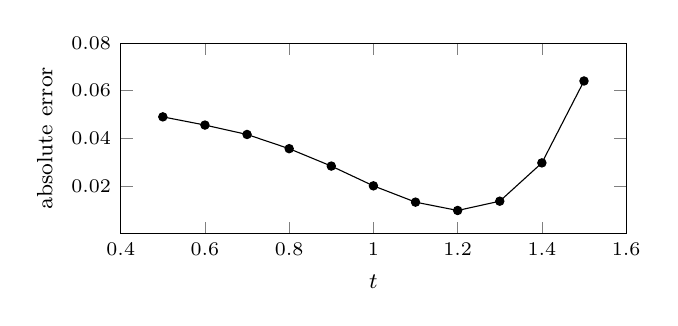
\begin{tikzpicture}
\begin{axis}[
    xlabel=\footnotesize{$t$},
    ylabel=\footnotesize{absolute error},
    xmin = 0.4, xmax = 1.6,
    xtick = {0.4,0.6,0.8,1.0,1.2,1.4,1.6},
    ymin = 0, ymax =0.08,
    ytick = {0.02,0.04,0.06,0.08},
    width=8cm,height=4cm,
    font = \scriptsize,
    scaled y ticks = false,
    yticklabel style={
            /pgf/number format/fixed,
        },
]
% \addplot[color=red]{exp(x)};
\addplot[mark=*,black,mark size=1.5pt] plot coordinates {
    (1.5,0.0641)
    (1.4,0.02969)
    (1.3,0.0136)
    (1.2,0.0097)
    (1.1,0.0132)    
    (1,0.02005)   
    (0.9,0.02835)   
    (0.8,0.03566)
    (0.7,0.04163)   
    (0.6,0.04558)   
    (0.5,0.04903)           
};
\end{axis}
\end{tikzpicture}

    \caption{Prediction on different time horizon.}
    \label{fig:prediction_time}
\end{figure}

We record the absolute error of PINN predictions across different time horizons as shown in Fig.~\ref{fig:prediction_time}. The absolute errors remain consistently small (less than 0.08) from $t = 0.5$ to $t = 1.5$ throughout the entire time span, suggesting the model is able to generalize to unseen time horizons with high accuracy. 

\subsection{PINN Performance with Different Training Epochs}

\begin{figure}[ht]
    \centering
    \begin{tikzpicture}
\begin{axis}[
    axis y line*=left,
    xlabel=\footnotesize{\# epoch},
    ylabel=\footnotesize{percentage error},
    xmin = 10000, xmax = 60000,
    xtick = {10000,20000,30000,40000,50000,60000},
    ymin = 0, ymax =12,
    ytick = {0,2,4,6,8,10,12},
    yticklabel={$\pgfmathprintnumber{\tick}\%$},
    width=8cm,height=4cm,
    scaled y ticks = false,
    yticklabel style={
            /pgf/number format/fixed,
        },
    font = \scriptsize
]
\addplot [mark=*, black, mark size=1.5pt]table[x=x,y=y] {pinn_epoch.dat};\label{plot_one}
% \addlegendentry{percentage error}
\end{axis}

% \addplot [name path=upper,draw=none] table[x=x,y expr=\thisrow{y}+\thisrow{err}] {pinn_epoch.dat};
% \addplot [name path=lower,draw=none] table[x=x,y expr=\thisrow{y}-\thisrow{err}] {pinn_epoch.dat};
% \addplot [fill=blue!10] fill between[of=upper and lower];

\begin{axis}[
    axis y line*=right,
    % xlabel=x-axis,
    ylabel=\footnotesize{absolute error},
    xmin = 10000, xmax = 60000,
    xtick = {10000,20000,30000,40000,50000,60000},
    ymin = 0.01, ymax =0.04,
    ytick = {0,0.01,0.02,0.03,0.04},
    width=8cm,height=4cm,
    scaled y ticks = false,
    yticklabel style={
            /pgf/number format/fixed,
        },
    font = \scriptsize
]
\addplot [mark=*, blue, mark size=1.5pt]table[x=x,y=err] {pinn_epoch.dat};\label{plot_two}
\addlegendimage{/pgfplots/refstyle=plot_one}\addlegendentry{percentage error}
\addlegendimage{/pgfplots/refstyle=plot_two}\addlegendentry{absolute error}
% \addlegendentry{absolute error}
\end{axis}
\end{tikzpicture}
    \caption{PINN with different epochs for training (\#domain = 600).}
    \label{fig:pinn_epoch}
\end{figure}
% \begin{table*}[]
% \begin{tabular}{ccccccc}
% \hline
% \multicolumn{1}{l|}{\# Epoch ($\times 10^{4}$)}           & 1                          & 2                          & 3                          & 4                           & 5                            & 6                            \\ \hline
% \multicolumn{1}{l|}{Prediction Error ($\times 10^{-2}$)} & 7.104$\pm$ 2.5882 & 5.322 $\pm$ 2.009 & 5.475 $\pm$ 2.065 & 5.940 $\pm$ 2.2517 & 4.7326 $\pm$ 1.8146 & 4.8094 $\pm$ 1.8371 \\ \hline                              
% \end{tabular}
% \end{table*}

\begin{table*}[t]
\small
\centering
\begin{tabular}{c|cccccc}
\Xhline{3\arrayrulewidth}
\# Epoch($\times 10^{4}$)          & 1                          & 2                          & 3      & 4   & 5   &6                   \\ \hline
Prediction Error ($\%$) & 7.104& 5.322  & 5.475  & 5.940 & 4.733 & 4.809 \\\hline
Absolute Error ($\times 10^{-2}$) & 2.588 & 2.009 &  2.065 & 2.252 &1.815&1.837\\\Xhline{3\arrayrulewidth}
\end{tabular}
\caption{PINN with different epochs for training}
\label{tab:pinn_epoch}
\end{table*}


Here, we assess the performance of the PINN across the amount of training epochs. We present the absolute error (absolute value of the difference between the PINN prediction and the ground truth) and the percentage error (absolute error over the ground truth value). Fig.~\ref{fig:pinn_epoch} and Table~\ref{tab:pinn_epoch} shows the results. 
% \todo{to decide} In Fig.~\ref{fig:pinn_epoch}, the blue shaded region indicates the absolute errors, while the line plot illustrates the average percentage error. 
The results suggest that PINN with long enough training epochs will yield accurate estimations, while further increasing training epochs (beyond  50000 epochs) will not give performance improvement.
% The results suggest that large neural networks with enough representation power will yield accurate estimations.

% \jacob{the absolute error is not the standard deviation for percentage error. I think we should present them separately. And we should keep either the figure or the table.}

% \jacob{The percentage error 0.05 in the google doc means 5\%}



\subsection{PINN Performance on Different PDE Constraints}

\begin{figure}[ht]
    \centering
    % \begin{tikzpicture}
% \begin{axis}[
%     xlabel=\footnotesize{\# domain},
%     ylabel=\footnotesize{percentage error},
%     xmin = 0, xmax = 2500,
%     xtick = {0,200,400,600,1200,2400},
%     ymin = 0, ymax =0.12,
%     ytick = {0.04,0.08,0.12},
%     width=8cm,height=4cm,
%     scaled y ticks = false,
%     yticklabel style={
%             /pgf/number format/fixed,
%         },
%     font = \scriptsize
% ]
% \addplot [mark=*, mark color=black, mark size=1.5pt]table[x=x,y=y] {pinn_pde.dat};

% \addplot [name path=upper,draw=none] table[x=x,y expr=\thisrow{y}+\thisrow{err}] {pinn_pde.dat};
% \addplot [name path=lower,draw=none] table[x=x,y expr=\thisrow{y}-\thisrow{err}] {pinn_pde.dat};
% \addplot [fill=blue!10] fill between[of=upper and lower];

% \end{axis}
% \end{tikzpicture}

\begin{tikzpicture}
\begin{axis}[
    axis y line*=left,
    xlabel=\footnotesize{\# domain},
    ylabel=\footnotesize{percentage error},
    xmin = 0, xmax = 2500,
    xtick = {0,200,400,600,1200,2400},
    ymin = 0, ymax =12,
    ytick = {0,2,4,6,8,10,12},
    yticklabel={$\pgfmathprintnumber{\tick}\%$},
    width=8cm,height=4cm,
    scaled y ticks = false,
    yticklabel style={
            /pgf/number format/fixed,
        },
    font = \scriptsize
]
\addplot [mark=*, black, mark size=1.5pt]table[x=x,y=y] {pinn_pde.dat};\label{plot1}
% \addlegendentry{percentage error}
\end{axis}

% \addplot [name path=upper,draw=none] table[x=x,y expr=\thisrow{y}+\thisrow{err}] {pinn_epoch.dat};
% \addplot [name path=lower,draw=none] table[x=x,y expr=\thisrow{y}-\thisrow{err}] {pinn_epoch.dat};
% \addplot [fill=blue!10] fill between[of=upper and lower];

\begin{axis}[
    axis y line*=right,
    % xlabel=x-axis,
    ylabel=\footnotesize{absolute error},
    xmin = 0, xmax = 2500,
    xtick = {0,200,400,600,1200,2400},
    ymin = 0.01, ymax =0.04,
    ytick = {0,0.01,0.02,0.03,0.04},
    width=8cm,height=4cm,
    scaled y ticks = false,
    yticklabel style={
            /pgf/number format/fixed,
        },
    font = \scriptsize
]
\addplot [mark=*, blue, mark size=1.5pt]table[x=x,y=err] {pinn_pde.dat};\label{plot2}
\addlegendimage{/pgfplots/refstyle=plot1}\addlegendentry{percentage error}
\addlegendimage{/pgfplots/refstyle=plot2}\addlegendentry{absolute error}
% \addlegendentry{absolute error}
\end{axis}
\end{tikzpicture}



    \caption{PINN with different numbers of PDE constraint grid points.}
    \label{fig:pinn_pde}
\end{figure}

% \begin{table*}[]
% \begin{tabular}{ccccccccc}
% \hline
% \multicolumn{1}{l|}{\# Domain}           & 100                          & 200                          & 300                         & 400                           & 500                            & 600     &1200       &2400                       \\ \hline
% \multicolumn{1}{l|}{Prediction Error ($\times 10^{-2}$)} & 5.4982$\pm$ 2.0817 & 5.391 $\pm$ 2.022523 & 5.7488 $\pm$ 2.171 & 5.9265 $\pm$ 2.2209 & 5.478 $\pm$ 2.058 & 5.283 $\pm$ 1.9888 & 5.1528 $\pm$ 1.962  & 4.992 $\pm$ 1.894  \\ \hline                              
% \end{tabular}
% \end{table*}


\begin{table*}[t]
\small
\centering
\begin{tabular}{ccccccccccccc}
\Xhline{3\arrayrulewidth}
\multicolumn{1}{l|}{\# Domain}           & 100                          & 200                          & 300                         & 400                & 500                            & 600     &1200       &2400                               \\ \hline
\multicolumn{1}{l|}{Prediction Error ($\%$)} & 5.498 & 5.391 & 5.749  & 5.927 & 5.478 & 5.283 & 5.153 & 4.992\\ \hline   
\multicolumn{1}{l|}{Absolute Error ($\times 10^{-2}$)} & 2.082 & 2.023 & 2.171 & 2.221 &2.058 &1.989 &1.962 &1.894 \\ \Xhline{3\arrayrulewidth}
% \multicolumn{1}{l|}{\# Domain}           & 500                            & 600     &1200       &2400                       \\ \hline
% \multicolumn{1}{l|}{Prediction Error ($\times 10^{-2}$)} & 5.478 $\pm$ 2.058 & 5.283 $\pm$ 1.989 & 5.153 $\pm$ 1.962  & 4.992 $\pm$ 1.894  \\ \hline  \hline
\end{tabular}
\caption{PINN with different numbers of PDE constraint grid points}
\label{tab:pinn_pde}
\end{table*}


\begin{table*}[!ht]
\small
\centering
\begin{tabular}{ccccccccccccc}
\Xhline{3\arrayrulewidth}
\multicolumn{1}{l|}{Network Architecture}           & [16]  & [64] & [128]                           \\ \hline
\multicolumn{1}{l|}{Feature Representation Error ($\%$)} & 0.248 & 0.250 & 0.251 \\ \hline   
\multicolumn{1}{l|}{Cost Reconstruction Error ($\%$)} & 0.901 & 0.984 & 1.003 \\ \Xhline{3\arrayrulewidth}

% \multicolumn{1}{l|}{\# Domain}           & 500                            & 600     &1200       &2400                       \\ \hline
% \multicolumn{1}{l|}{Prediction Error ($\times 10^{-2}$)} & 5.478 $\pm$ 2.058 & 5.283 $\pm$ 1.989 & 5.153 $\pm$ 1.962  & 4.992 $\pm$ 1.894  \\ \hline  \hline
\end{tabular}
 \caption{Autoencoder-like network architecture for $n_{\text{layer}}=1$}
\label{tab:n_layer = 1}
\end{table*}
\begin{table*}[!ht]
\small
\centering
\begin{tabular}{ccccccccccccc}
\Xhline{3\arrayrulewidth}
\multicolumn{1}{l|}{Network Architecture}           & [16, 64, 16]  & [64, 64, 64] & [64, 128, 64]                           \\ \hline
\multicolumn{1}{l|}{Representation Error ($\%$)} & 0.112 & 0.394 & 0.119 \\ \hline   
\multicolumn{1}{l|}{Cost Reconstruction Error ($\%$)} & 0.868 & 0.880 & 0.371 \\ \Xhline{3\arrayrulewidth}

% \multicolumn{1}{l|}{\# Domain}           & 500                            & 600     &1200       &2400                       \\ \hline
% \multicolumn{1}{l|}{Prediction Error ($\times 10^{-2}$)} & 5.478 $\pm$ 2.058 & 5.283 $\pm$ 1.989 & 5.153 $\pm$ 1.962  & 4.992 $\pm$ 1.894  \\ \hline  \hline
\end{tabular}
\caption{Autoencoder-like network architecture for $n_{\text{layer}}=3$}
\label{tab:n_layer = 3}
\end{table*}
\begin{table*}[!ht]
\small
\centering
\begin{tabular}{ccccccccccccc}
\Xhline{3\arrayrulewidth}
\multicolumn{1}{l|}{Network Architecture}           & [16, 64, 128, 64, 16]  & [64, 64, 128, 64, 64] & [64, 128, 128, 128, 64]                     \\ \hline
\multicolumn{1}{l|}{Representation Error ($\%$)} & 0.007 & 0.011 & 0.009 \\ \hline   
\multicolumn{1}{l|}{Cost Reconstruction Error ($\%$)} & 0.120 & 0.099 & 0.129 \\ \Xhline{3\arrayrulewidth}

% \multicolumn{1}{l|}{\# Domain}           & 500                            & 600     &1200       &2400                       \\ \hline
% \multicolumn{1}{l|}{Prediction Error ($\times 10^{-2}$)} & 5.478 $\pm$ 2.058 & 5.283 $\pm$ 1.989 & 5.153 $\pm$ 1.962  & 4.992 $\pm$ 1.894  \\ \hline  \hline
\end{tabular}
\caption{Autoencoder-like network architecture for $n_{\text{layer}}=5$}
\label{tab:n_layer = 5}
\end{table*}

We also examine the performance of the PINN with different PDE loss configurations. We fix the training epochs to be 60000 and vary the number of grid points for imposing PDE constraints for PINN training. We present the results in Fig.~\ref{fig:pinn_pde} with the numerical results shown in Table~\ref{tab:pinn_pde}. 
% In Fig.~\ref{fig:pinn_pde}, the blue shaded region indicates the absolute errors, while the line plot illustrates the average percentage error. 
We can see the error drops as the PDE constraint is imposed with finer grids, but quickly saturates. For optimal training efficiency, we suggest to select a moderate number of grid points for PDE constraints in the PINN to balance accuracy with computation time. 

\section{Representation Learning with Autoencoder-like Neural Networks}

In this section, we provide details on the experiments presented in the paper on the autoencoder-like neural network.

\subsection{Algorithm Details}

\begin{algorithm*}[t]
\caption{Autoencoder-like Neural Network Training}\label{alg:auto-encoder_training}
\begin{algorithmic}[1]
% add comments for each line
\State \textbf{Given:} $w_{RC}, w_{C.T.}, k, d, \alpha$ \Comment{$d$ is the frequency for preimage update, $\alpha$ is the initial learning rate}
\For {each epoch}
    \For {each batch}
        \State $\hat{r}(\boldsymbol\xi), \boldsymbol\xi \gets \textrm{AE}(\mathcal{X})$ \Comment{pass the batched state-space samples $\mathcal{X}$ to the autoencoder-like network AE to get $\hat{r}(\boldsymbol\xi), \boldsymbol\xi$} \label{line: AE pass}
        \If {$d$ batches have passed $\mathbf{or}$ first batch} \label{line:every_d_iter}
            \State $\mathcal{R}\gets\textrm{range}(\boldsymbol p)$ \Comment{find $\mathcal{R}$, the range of each $p_i$ for $i\in[k]$}
            \State 
            $\mathcal{M}_{\boldsymbol\xi} \gets \textrm{preimage}(\mathcal{X}, \boldsymbol\xi)$ \Comment{find $\mathcal{M}_{\boldsymbol\xi}$, the preimage of each $\boldsymbol\xi^{(i)}$ for $i\in[k]$} \label{line: preimage}
        \EndIf
        \State $\mathcal{L}_{RC}(\boldsymbol\theta) = \frac{1}{|\mathcal{X}|}\sum_{x\in\mathcal{X}}\left(c(x)-\hat{r}(\boldsymbol\xi; \boldsymbol\theta)\right)^2$ \Comment{running-cost/barrier function reconstruction loss} \label{line: RC loss}
        \State $ \mathcal{L}_{C.T.}(\boldsymbol\theta) = \frac{1}{k}\sum_{i=1}^k\frac{1}{|\mathcal{R}_i|}\sum_{\xi\in\mathcal{R}_i}\frac{1}{|\mathcal{M}_{\xi, i}|}$ \Comment{comparison theorem loss} \label{line: CT loss}
        \State \qquad\qquad\qquad\qquad
        $\ldots \sum_{x\in\mathcal{M}_{\xi, i}}
          ||\nabla_x a_i(x; \boldsymbol\theta) ||_2^2 + || \nabla_x b_i(x; \boldsymbol\theta)||_2^2$
        \State $\mathcal{L}_{AE}(\boldsymbol\theta)=w_{RC}\mathcal{L}_{RC}(\boldsymbol\theta)+w_{C.T.}\mathcal{L}_{C.T.}(\boldsymbol\theta)$ \Comment{total loss for the autoencoder} \label{line: total loss}
        \State $\boldsymbol\theta\gets\textrm{Adam}(\boldsymbol\theta, \alpha)$ \Comment{parameters update with the Adam optimizer}
    \EndFor
\EndFor
    
\end{algorithmic}
\end{algorithm*}

% \todo{change reference to line~\ref{line:every_d_iter}}

We present details of the training procedure for the proposed autoencoder-like neural network (Fig. \ref{fig:AE diagram}) to automatically identify lower-dimensional features in Algorithm~\ref{alg:auto-encoder_training}. We use boldface symbols to denote the vector of such symbols (\eg $\boldsymbol\xi = [\boldsymbol\xi^{(1)}, \boldsymbol\xi^{(2)}, \ldots, \boldsymbol\xi^{(k)}]$, and $\boldsymbol\xi^{(1)}=[\xi_1^{(1)}, \xi_2^{(1)}, \ldots]^\top$). 

First, we partition the state-space training data into appropriately sized batches, $\mathcal{X}$. This batch is then passed into the autoencoder (line~\ref{line: AE pass}), where the encoder returns $\hat{\boldsymbol\xi}$ and the decoder returns $\hat{r}(\boldsymbol\xi)$. In order to obtain the comparison theorem loss in~\eqref{eq: CT loss}, we must calculate gradients over the preimage of each $\xi\in\mathcal{R}_i$.
%, defined as $\mathcal{M}_{\xi, i}=\{x: p_i(x; \boldsymbol\theta)=\xi\}$. 
Retrieving this set requires a method for inverting the encoder $p_i(x)$, and we approximate the preimage using a grid-search over the state-space (line~\ref{line: preimage}).
However, such a search can impose a high computational burden on the training regime, and to address this issue we update the preimage only after every $d$ batches (line~\ref{line:every_d_iter}). 
% which imposes a high computational burden on the training regime.
% and only update this preimage every $d$ batches in order to avoid the preimage computation at every iteration (line 5). 
Thus, the comparison theorem loss in line~\ref{line: CT loss} uses the same (outdated) preimage for the following $d$ iterations. In the simulation described in the paper, we set $d=1$ since the preimage computation is not very expensive for the 3-dimensional system. However, for larger systems, it will become necessary to update the preimage sparsely to avoid the grid-search (or an alternative polyhedral computation~\cite{polyhedral}) over the high-dimensional state-space. 

Due to the discretization in $\mathcal{X}$, the preimage function in line~\ref{line: preimage} assumes a threshold $\epsilon$ for which 
$$|p_j(x_a) - p_j(x_b)|<\epsilon\implies \xi_a^{(j)}=\xi_b^{(j)},$$
where $a$ and $b$ are distinct samples of the state-space and $p_j(x)$ is the $j^{th}$ feature map of $k$ such maps. We choose $\epsilon$ empirically such that the encoder $p(x)$ is a many-to-one mapping, \ie $p_j: \mathcal{X}\in\mathbb{R}^{N\times n}\mapsto\boldsymbol\xi^{(j)}\in\mathbb{R}^{M\times 1}$, where $N$ is the number of state-space observations in $\mathcal{X}$, $M$ is the number of distinct feature observations $\boldsymbol{\xi}^{(j)}$ according to the threshold $\epsilon$, and $M\ll N$. In 3-dimensional example considered in the paper ($n=3$), $\epsilon_j=\frac{1}{5}\frac{1}{N-1}\sum_{i=1}^{N-1}|\xi_{i+1}^{(j)}-\xi_i^{(j)}|$, which results in $M\approx 15$ for $N=1000$.

In line~\ref{line: RC loss}, we calculate the reconstruction loss~\eqref{eq: RC loss} that quantifies how well the learned features $\boldsymbol\xi$ represent the cost function. The total loss in line~\ref{line: total loss} is the weighted sum of the reconstruction loss and the comparison theorem loss. The weights $w_{C.T.}$ and $w_{RC}$ should be chosen to ensure that $w_{C.T.}\mathcal{L}_{C.T.}$ and $w_{RC}\mathcal{L}_{RC}$ are similar in magnitude. In our test case, the state-space domain is $[0, 1]^3$
% \todo{double check, I believe it's something else for the PINN and MC experiments. Reece: I meant the autoencoder test case. for the pinn/MC, you evaluate it over a larger state-space, but the autoencoder is tested over $[0,1]^3$}
sampled at a spatial resolution of 0.01. Due to the smoothness feature of the encoder, the preimage $\mathcal{M}_{\xi, i}$ of any individual feature observation will have state-space observations contained in a small neighborhood whose density and width is determined by the sampling resolution and the threshold $\epsilon$, respectively. 
% \todo{need to clarify the logic, why state space domain gives small jacobians and hessian?} 
The Jacobians and Hessians needed to calculate $a(x)$ and $b(x)$ over this neighborhood could be small in magnitude, resulting in smaller $\mathcal{L}_{C.T.}$ relative to $\mathcal{L}_{RC}$. Thus, we choose $w_{C.T.}=1$ and $w_{RC}=10$ for our test case.  
% weights should be chosen appropriately to ensure the comparison theorem loss sufficiently influences the total loss so that optimization of the network parameters $\boldsymbol{\theta}$ represents a meaningful minimization of $\mathcal{L}_{C.T.}$. 



\subsection{Network Performance on Different Training Regimes}
In this section, we compare the representation learning results for different network architectures in the proposed autoencoder-like model to examine its effect on performance. The network settings we consider are different hidden layer numbers and different numbers of neurons per layer. Recall the the basic model architecture contains two components: the encoder subarchictecture and the encoder subarchictecture. The encoder architecture consists of an projection from the system dimension to a high-dimensional space, followed by a projection down to the desired feature dimension. The decoder architecture is identical, only the down-projection is to a scalar value that represents the networks prediction of the cost/barrier function. Thus, to configure the network, we consider a different number of layers and neurons per layer in the up-projection and down-projection regions separately. For all experiments, we train the network on a $[0, 1]^3$ state-space with grid-size 0.01 using the Adam optimizer~\cite{kingma2017adam} with initial learning rate 0.001 and Glorot uniform initialization for the network parameters. The network is trained for 5 epochs with batch size of 1000 for 100 iterations. 

To examine the effect of the network architecture on feature learning, we begin with the encoder architecture and fix the number of layers in the decoder architecture at two, with 10 and 100 neurons respectively. We consider the number of layers in the encoder architecture as $n_{\text{layer}}\in[1, 3, 5]$. For each layer configuration, we consider the number of neurons per layer as $n_{\text{unit}}\in[16, 64, 128]$. Tables~\ref{tab:n_layer = 1}--\ref{tab:n_layer = 5} report the percent error of the learned features for different layer numbers and neurons per layer. It is clear that a wider network (more layers) learns features with error orders of magnitude lower than the shallow network experiments, yet sacrifices in computation time. 


To examine the effect of the network architecture on cost function reconstruction, we fix the number of layers in the encoder architecture at two, with 10 and 100 neurons respectively. Experiments on the decoder architecture yield similar results (Tables~\ref{tab:n_layer = 1}--\ref{tab:n_layer = 5}). Increasing the number of neurons per layer had little effect on the ability of the model to reconstruct the cost function. However, wider networks consistently achieved lower percent error between the ground truth cost function and the predicted cost function. 

Thus, we find that the performance of the network quickly saturates at a relatively low number of units per layer. Best performance is observed when the encoder and decoder architecture are symmetric, with a significant gain in prediction accuracy in wider networks. 

%To retain the basic model architecture that allows feature learning and cost/barrier function reconstruction, we require at least 3 hidden layers. The first hidden layer is a projection from the original system dimension $n$ to a high dimensional space, which is required if the dimension of the desired representation $k$ is on a similar scale as $n$. That is, $n\approx k$. 


% \bibliography{aaai24}

\end{document}
